 
 
 

\chapter{Sequences and Series of Functions}\label{ch6}

 In this chapter, we   study sequences and series whose terms depend on a variable. 
 
\section{Convergence of Sequences and Series of Functions}\label{sec6.1}
Let $D$ be a subset of real numbers. For each positive integer $n$, let $f_n:D\to\mathbb{R}$ be a function defined on $D$. Then $\{f_n\}_{n=1}^{\infty}$ is a sequence of functions defined on $D$. Sometimes we will write $\{f_n:D\to\mathbb{R}\}$ or  $\{f_n:D\to\mathbb{R}\}_{n=1}^{\infty}$ to make it explicit that each $f_n$ is a function defined on $D$. 

Given a sequence of functions $\{f_n:D\to\mathbb{R}\}$ that are defined on $D$, for each $x\in D$, $\{f_n(x)\}$ is a sequence of real numbers. We can determine whether such a sequence is convergent.

\begin{definition}{Pointwise Convergence of Sequence of Functions}
Given a sequence of functions $\{f_n:D\to\mathbb{R}\}$ that are defined on $D$, we say that it {\bf converges pointwise} to the function $f:D\to\mathbb{R}$ provided that  for every $x\in D$, the sequence $\{f_n(x)\}$ converges to $f(x)$. Namely,
\[f(x)=\lim_{n\to\infty}f_n(x)\hspace{1cm}\text{for all}\;x\in D.\]In this case, we also say that the function $f:D\to\mathbb{R}$ is the pointwise limit of the sequence of functions $\{f_n:D\to\mathbb{R}\}$.
\end{definition}
 
 Let us look at some examples.
\begin{example}[label=230303_1]{}
 For each positive integer $n$, let $f_n:[0,1]\to\mathbb{R}$ be the function $f_n(x)=x^n$. Study the pointwise convergence of the sequence of functions $\{f_n\}$.
\end{example}
\begin{solution}{Solution}Notice that
 \[\lim_{n\to\infty}x^n=\begin{cases}0,\quad &\text{if}\;0\leq x<1,\\1,\quad &\text{if}\;\quad x=1.\end{cases}\] 
Therefore, the sequence of functions $\{f_n\}$ converges pointwise to the function $f:[0,1]\to\mathbb{R}$, where
 \[f(x)=\begin{cases}0,\quad &\text{if}\;0\leq x<1,\\1,\quad &\text{if}\;\quad x=1.\end{cases}\]
\end{solution}

 
\begin{figure}[ht]
\centering
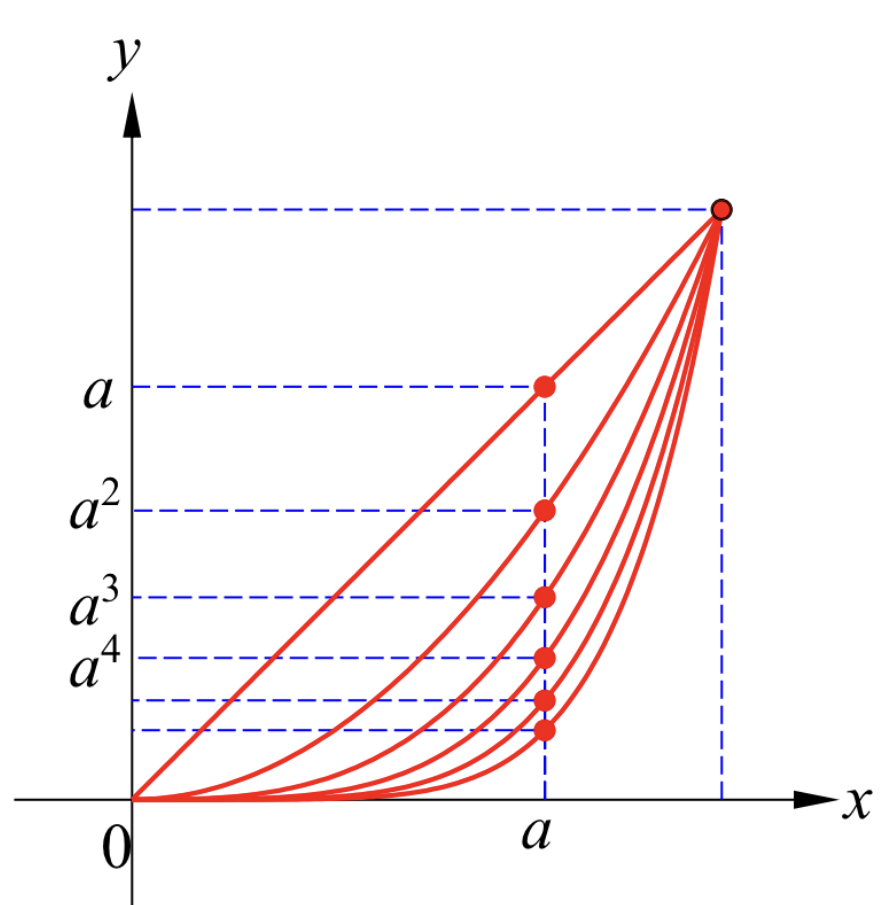
\includegraphics[scale=0.2]{Picture52.png}
\caption{The sequence of functions $\{f_n\}$ defined in Example \ref{230303_1}.\fa}\label{figure52}
\end{figure}


\begin{example}[label=230303_2]{}
 For each positive integer $n$, let $f_n:[0,2]\to\mathbb{R}$ be the function $f_n(x)=x^n$. Study the pointwise convergence of the sequence of functions $\{f_n\}$.\end{example}
\begin{solution}{Solution}
  For each $x\in [0,1]$, the sequence $\{f_n(x)\}$ is convergent. For any $x\in (1, 2]$, the sequence $\{f_n(x)\}$ is divergent. Hence, the sequence of functions $\{f_n\}$ does not converge pointwise.
\end{solution}
\begin{highlight}{}
In Example \ref{230303_1}, notice that each   $f_n:[0,1]\to\mathbb{R}$  is a  continuous function, but the limit  $f:[0,1]\to\mathbb{R}$ is not  a continuous function.

 Given that $\{f_n:D\to\mathbb{R}\}$ is a sequence of functions that converges pointwise to the function $f:D\to\mathbb{R}$.  We will consider the following questions.
\begin{enumerate}[1.]
\item If each $f_n$ is continuous, is $f$ continuous?
\item If each $f_n$ is a differentiable function defined on an open interval $I$, is $f$ differentiable on $I$? If yes, does the sequence $\{f_n':I\to\mathbb{R}\}$ converge to $f':I\to\mathbb{R}$?
\item If each $f_n$ is Riemann  integrable on a closed and bounded interval $I$, is $f$ Riemann integrable on $I$? If yes, does 
the sequence of integrals $\di\left\{\int_If_n \right\}$ converge to the integral $\di\int_I f$?
\end{enumerate}We have seen that the answer to the first question is no, as given by Example \ref{230303_1}. The answers to the second  and third questions are also no. We will look at some examples.
\end{highlight}
 
 
\begin{example}[label=230303_3]{}
 For each positive integer $n$, let $f_n:\mathbb{R}\to\mathbb{R}$ be the function \[f_n(x)=\frac{1}{1+nx^2}.\]
  Study the pointwise convergence of the sequence of functions $\{f_n\}$.

\end{example}
\begin{solution}{Solution}Since $f_n(0)=1$ for all $n\in\mathbb{Z}^+$,
\[
\lim_{n\to\infty}f_n(0)=1.
\]If $x\neq 0$, 
\[0\leq f_n(x)\leq \frac{1}{nx^2}.\] \bs
By squeeze theorem,
\[\lim_{n\to\infty}f_n(x)=0\hspace{1cm}\text{when}\;x\neq 0.\]
Hence, the sequence  of functions $\{f_n\}$ converges pointwise to the function $f:\mathbb{R}\to\mathbb{R}$, where
 \[f(x)=\begin{cases}0,\quad &\text{if}\;x\neq 0,\\1,\quad &\text{if}\; x=0.\end{cases}\]
\end{solution}


\begin{figure}[ht]
\centering
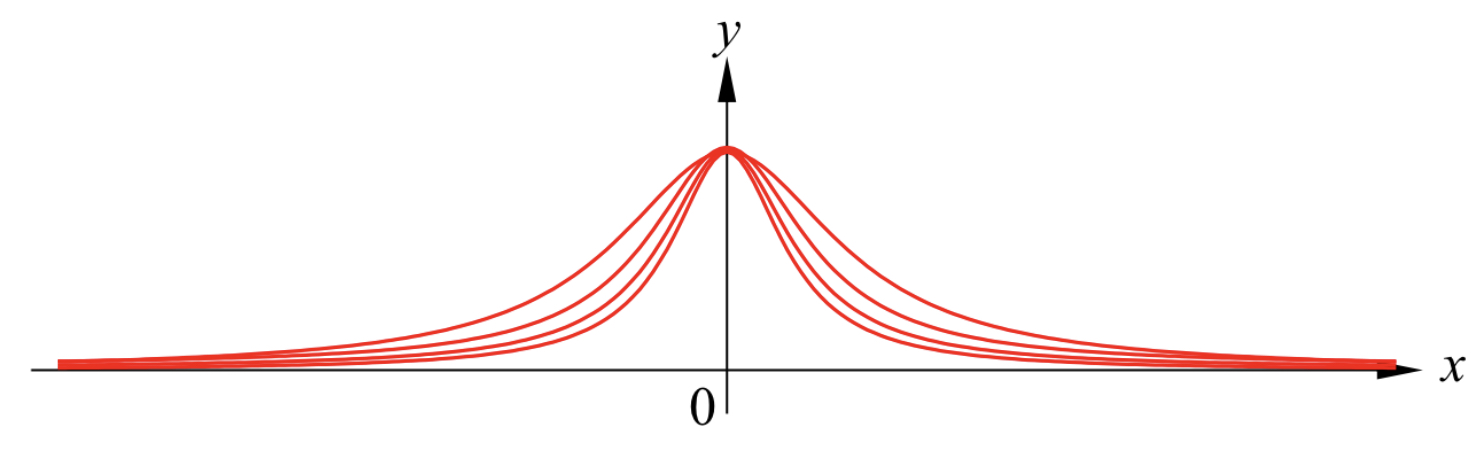
\includegraphics[scale=0.18]{Picture53.png}
\caption{The sequence of functions $\{f_n\}$ defined in Example \ref{230303_3}.\fa}\label{figure53}
\end{figure}

\begin{highlight}{}
In Example \ref{230303_3}, each of the functions $f_n$ is differentiable. But the function $f$ is not differentiable at $x=0$ since it is not continuous at $x=0$.

\end{highlight}

\begin{example}[label=230303_4]{}
 For each positive integer $n$, let $f_n:\mathbb{R}\to\mathbb{R}$ be the differentiable function \[f_n(x)=xe^{-nx^2}.\]
 \begin{enumerate}[(a)]
 \item  Study the pointwise convergence of the sequence of functions $\{f_n\}$.
 
 \item Study the pointwise convergence of the sequence of functions $\{f_n'\}$.
 \end{enumerate}
\end{example}
\begin{solution}{Solution}
\begin{enumerate} [(a)]
 
\item Since $f_n(0)=0$ for all $n\in\mathbb{Z}^+$,
\[
\lim_{n\to\infty}f_n(0)=0.
\]\end{enumerate}\bs \begin{enumerate}[]\item If $x\neq 0$, since $\di\lim_{u\to\infty}e^{-u}=0$, we find that
\[\lim_{n\to\infty}f_n(x)=x\lim_{n\to\infty}e^{-nx^2}=x\lim_{u\to \infty}e^{-u}=0.\]
Hence, the sequence of functions $\{f_n\}$ converges pointwise to the function $f:\mathbb{R}\to\mathbb{R}$, where $f(x)=0$ for all $x\in\mathbb{R}$.\end{enumerate}\begin{enumerate}[(b)]
\item For $n\in\mathbb{Z}^+$, 
\[f_n'(x)=(1-2nx^2)e^{-nx^2}.\]
Since $f_n'(0)=1$ for all $n\in\mathbb{Z}^+$,
\[
\lim_{n\to\infty}f_n'(0)=1.
\]If $x\neq 0$, since  $\di\lim_{u\to\infty} e^{-u}=0$ and $\di\lim_{u\to\infty}ue^{-u}=0$, we find that
\[\lim_{n\to\infty}f_n'(x)= \lim_{n\to\infty}(1-2nx^2)e^{-nx^2}= \lim_{u\to \infty}(1-2u)e^{-u}=0.\] 
Hence, the sequence of functions $\{f_n'\}$ converges pointwise to the function $g:\mathbb{R}\to\mathbb{R}$, where  \[g(x)=\begin{cases}0,\quad &\text{if}\;x\neq 0,\\1,\quad &\text{if}\; x=0.\end{cases}\]
\end{enumerate}
\end{solution}


\begin{figure}[ht]
\centering
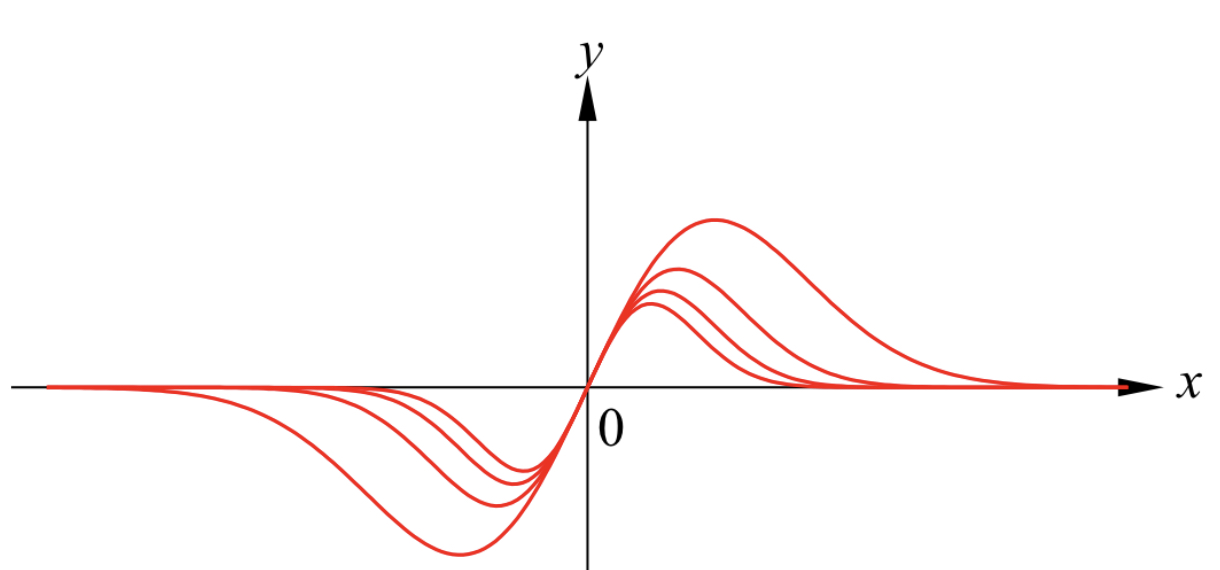
\includegraphics[scale=0.18]{Picture54.png}
\caption{The sequence of functions $\{f_n\}$ defined in Example \ref{230303_4}.\fa}\label{figure54}
\end{figure}

\begin{figure}[ht]
\centering
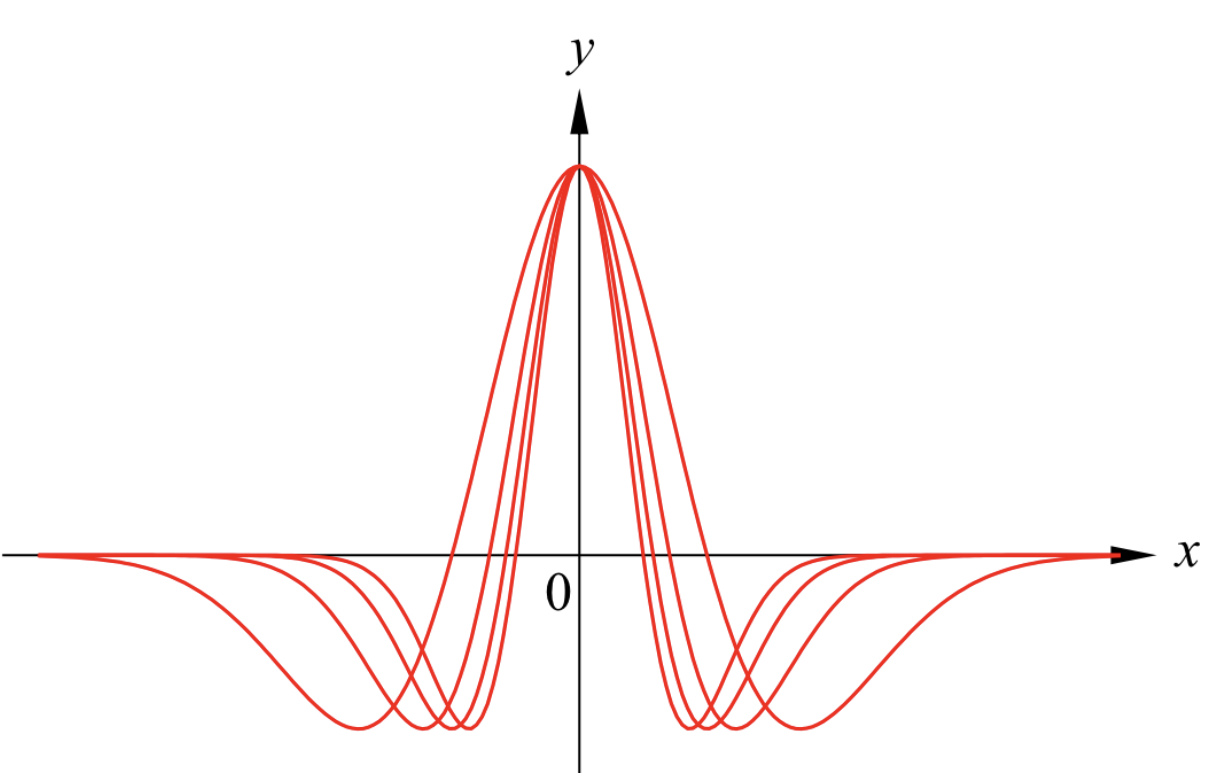
\includegraphics[scale=0.18]{Picture55.png}
\caption{The sequence of functions $\{f_n'\}$  in Example \ref{230303_4}.\fa}\label{figure55}
\end{figure}

\begin{highlight}{}
In Example \ref{230303_4}, each of the functions $f_n$ is differentiable and the  function $f$ is also differentiable. The sequence $\{f_n'\}$ also converges pointwise, but it does not converge to the function $f'$.

\end{highlight}

\begin{example}[label=230303_5]{}
 For each positive integer $n$, let 
 \[S_n=\left\{\left.\frac{p}{q}\,\right|\, p, q\in\mathbb{Z},\,0\leq p\leq q\leq n, q\geq 1\right\}.\]
 Define the function $f_n:[0,1]\to\mathbb{R}$ by
 \[f_n(x)=\begin{cases} 1,\quad &\text{if}\; x\in S_n,\\0,\quad &\text{if}\; x\notin S_n.\end{cases}\]Study the pointwise convergence of the sequence of functions $\{f_n\}$.
\end{example}
\begin{solution}{Solution}
If $x$ is a rational number in $[0,1]$, there exists a nonnegative integer  $p$ and a positive integer $q$ such that $0\leq p\leq q$ and $x=p/q$. Therefore, $x\in S_n$ for all $n\geq q$. This implies that 
$f_n(x)=1$ for all $n\geq q$. Hence,
\[\lim_{n\to\infty}f_n(x)=1\hspace{1cm}\text{if $x$ is rational}.\]\bs 
If $x$ is not a rational number, then $x\notin S_n$ for any $n\in\mathbb{Z}^+$. Therefore, $f_n(x)=0$ for all $n\in\mathbb{Z}^+$. Hence,
\[\lim_{n\to\infty}f_n(x)=0\hspace{1cm}\text{if $x$ is irrational}.\]These show that the sequence of functions $\{f_n\}$ converges pointwise to the Dirichlet function $f:\mathbb{R}\to\mathbb{R}$,
\[f(x)=\begin{cases}1,\quad &\text{if $x$ is rational},\\
0,\quad & \text{if $x$ is irrational}.\end{cases}.\]
\end{solution}
\begin{highlight}{}
For each $n\in\mathbb{Z}^+$, the set $S_n$ which  $f_n(x)\neq 0$ is  finite. Thus the function $f_n:[0,1]\to\mathbb{R}$ is  Riemann integrable. But the Dirichlet function $f$ is not Riemann integrable.
\end{highlight}


\begin{example}[label=230303_6]{}
 For each positive integer $n$, let 
 \[f_n(x)=\begin{cases} n^2x(1-nx),\quad &\text{if}\;0\leq x\leq \frac{1}{n},\\0,\quad  &\text{otherwise}.\end{cases}\] Notice that $f_n$ is integrable on $[0,1]$. Let
$\di c_n=\int_0^1f_n(x)dx$. 
 \begin{enumerate}[(a)]
 \item Study the pointwise convergence of the sequence of functions $\{f_n\}$.
\item Determine the limit of the sequence $\{c_n\}$.
\end{enumerate}
\end{example}
\begin{solution}{Solution}
\begin{enumerate}[(a)]
\item  Since $f_n(0)=0$ for all $n\in\mathbb{Z}^+$,
\[
\lim_{n\to\infty}f_n(0)=0.
\]
\end{enumerate}\bs \begin{enumerate}[]\item
If $x>0$, there is  a positive integer $N$ so that $x>1/N$. This implies that $f_n(x)=0$ for all $n\geq N$. Hence, we also have 
\[
\lim_{n\to\infty}f_n(x)=0.
\]Thus, the sequence of functions $\{f_n\}$ converges pointwise to the function $f:\mathbb{R}\to\mathbb{R}$, where $f(x)=0$ for all $x\in\mathbb{R}$.\end{enumerate}\begin{enumerate}[(b)]
\item We compute $c_n$ directly. For $n\in\mathbb{Z}^+$,
\[c_n=n^2\left[\frac{x^2}{2}-\frac{nx^3}{3}\right]_0^{1/n}=\frac{1}{6}.\]
Hence, the sequence $\{c_n\}$ converges to $1/6$.
\end{enumerate}
\end{solution}
\begin{highlight}{}
In Example \ref{230303_6},   each of the functions $f_n$ is integrable and the  function $f$ is also integrable. However, $\di\left\{\int_0^1f_n\right\}$ does not converge to $\di\int_0^1f$. 

\end{highlight}
\begin{figure}[ht]
\centering
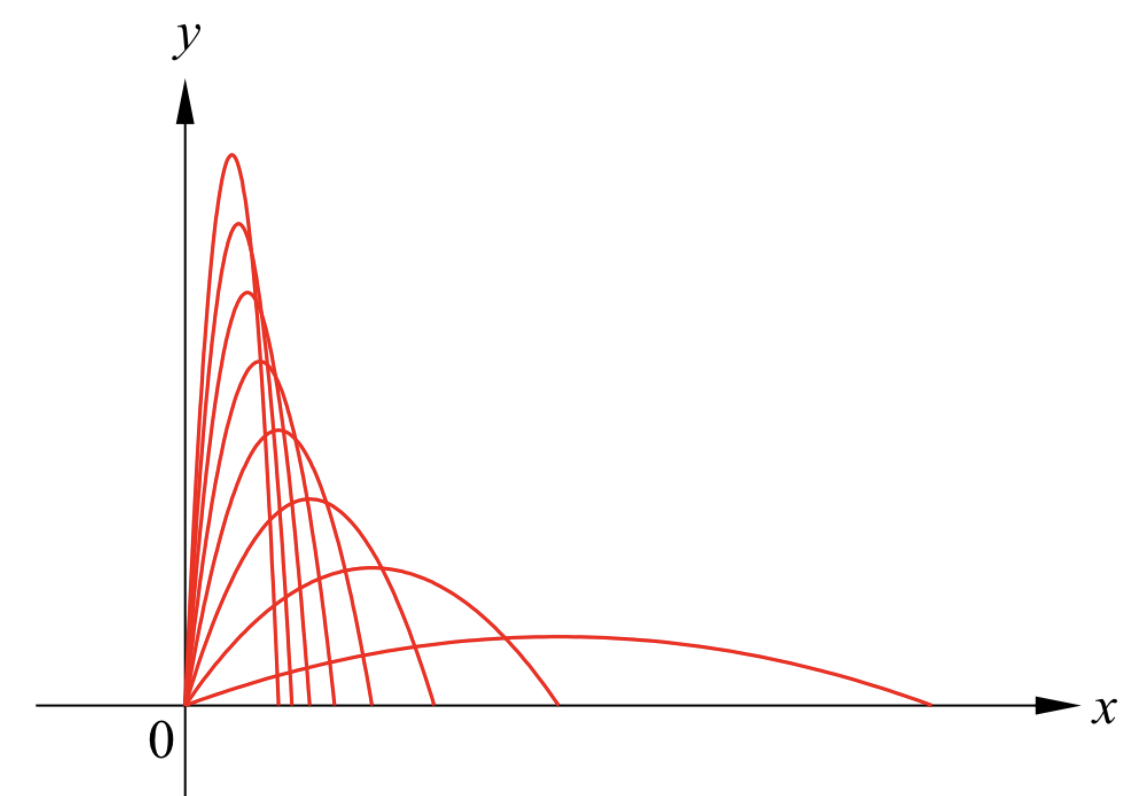
\includegraphics[scale=0.2]{Picture56.png}
\caption{The sequence of functions $\{f_n\}$ defined in Example \ref{230303_6}.\fa}\label{figure56}
\end{figure}

Now let us consider series of functions.
\begin{definition}{Pointwise Convergence of Series of Functions}
A series of functions defined on a set $A$ is a series of the form
\[\sum_{n=1}^{\infty}f_n(x),\]
where $\{f_n:A\to\mathbb{R}\}$ is a sequence of functions defined on $A$. For such a series, we form the partial sum
\[s_n(x)=\sum_{k=1}^n f_k(x)\hspace{1cm}\text{for}\;n\geq 1.\]
Then $\{s_n:A\to\mathbb{R}\}$ is a sequence of functons defined on $A$. The {\bf domain of convergence} of the series $\di\sum_{n=1}^{\infty}f_n(x)$ is the set
\[D=\left\{x\in A\,|\, \text{the sequence $\{s_n(x)\}$ is convergent}\right\}.\]
It is the largest subset $D$ of $A$ such that the sequence of functions
$\{s_n:D\to\mathbb{R}\}$ converges pointwise.  
For each $x$ in   $D$, let \[s(x)=\sum_{n=1}^{\infty}f_n(x)=\lim_{n\to\infty}s_n(x)\]
be the sum of the series. Then the  sequence of functions
$\{s_n:D\to\mathbb{R}\}$ converges pointwise to the function $s(x)$.
\end{definition}

 Let us reformulate Theorem \ref{230227_2} using series of functions.
\begin{example}[label=230305_16]{Geometric Series}
For the series $\di\sum_{n=0}^{\infty}x^n$, the terms are the functions $f_n(x)=x^n$, $n\geq 0$. They  are defined on $A=\mathbb{R}$. The partial sums are
\[s_n(x)=1+x+\cdots+x^n=\begin{cases}\di\frac{1-x^{n+1}}{1-x},\quad &\text{if}\;x\neq 1,\\n+1,\quad &\text{if}\;x=1.\end{cases}\]\be
The domain of convergence is the set $D=(-1,1)$. For $x\in D$, 
\[s(x)=\sum_{n=0}^{\infty}x^n=\frac{1}{1-x}.\]
Hence, the series of functons $\di\sum_{n=0}^{\infty}x^n$ converges pointwise on the interval $(-1,1)$ to the function $\di s(x)=\frac{1}{1-x}$.
\end{example2}

\begin{example}[label=230304_4]{}
Determine the domain of convergence of the series $\di\sum_{n=1}^{\infty}e^{-n^2 x}$.
\end{example}
\begin{solution}{Solution}
If $x\leq 0$, $-n^2x\geq 0$ for all $n\in\mathbb{Z}^+$. Therefore, $\di\lim_{n\to\infty}e^{-n^2 x}\neq 0$, and so the series $\di\sum_{n=1}^{\infty}e^{-n^2x}$ is divergent.

If $x>0$,  $\di\lim_{n\to\infty}e^{-n^2 x}=0$. In this case, notice that $n^2\geq n$  for all $n\in\mathbb{Z}^+$ implies that
\[0\leq e^{-n^2x}\leq e^{-nx}\hspace{1cm}\text{for all}\;n\in\mathbb{Z}^+.\]
Since the series $\di\sum_{n=1}^{\infty}e^{-nx}$ is a geometric series with positive constant ratio $r=e^{-x}<1$, it is convergent. By the comparison test, the series  $\di\sum_{n=1}^{\infty}e^{-n^2x}$ is also convergent.

 Therefore, the domain of convergence of the series  $\di\sum_{n=1}^{\infty}e^{-n^2 x}$ is $D=(0, \infty)$.
\end{solution}
\vp


\noindent
{\bf \large Exercises  \thesection}
\setcounter{myquestion}{1}
\begin{question}{\themyquestion}
 For each positive integer $n$, let $f_n:\mathbb{R}\to\mathbb{R}$ be the function defined by
 \[f_n(x)=e^{-nx^2}.\]  
   \begin{enumerate}[(a)]
   \item
  Determine the pointwise convergence of the sequence  of functions $\{f_n\}$.
 \item   Determine the pointwise convergence of the sequence of functions  $\{f_n'\}$.
 \end{enumerate}
\end{question}

\atc
\begin{question}{\themyquestion}
 For each positive integer $n$, let $f_n:(0,\infty)\to\mathbb{R}$ be the function defined by
 \[f_n(x)=\frac{1}{1+x^n}.\]  
  \begin{enumerate}[(a)]
   \item
  Determine the pointwise convergence of the sequence  of functions $\{f_n\}$.
 \item   Determine the pointwise convergence of the sequence of functions  $\{f_n'\}$.
 \end{enumerate}
\end{question}

\atc
\begin{question}{\themyquestion}
For each positive integer $n$, let $f_n:[0,\infty)\to\mathbb{R}$ be the function defined by
 \[f_n(x)=\frac{x}{1+nx},\]and  let
$\di c_n=\int_0^1f_n(x)dx$. 
\begin{enumerate}[(a)]
   \item  Determine the pointwise  convergence of the sequence of functions $\{f_n\}$.
   \item Determine the  convergence of the sequence $\{c_n\}$.
 \end{enumerate}
\end{question}
 


\atc
\begin{question}{\themyquestion}
For each positive integer $n$, let $f_n:\mathbb{R}\to\mathbb{R}$ be the function defined by
 \[f_n(x)=n\sin\left(\frac{x}{n}\right),\]  
 and let
$\di c_n=\int_0^1f_n(x)dx$.
\begin{enumerate}[(a)]
 \item  Study the  convergence of the sequence  of functions $\{f_n\}$.
\item  Study the  convergence of the sequence  of functions  $\{f_n'\}$.
\item Determine the limit of the sequence $\{c_n\}$.
 \end{enumerate}
\end{question}
 
 
 \atc
\begin{question}{\themyquestion}Find the domain of convergence of the series of functions $\di\sum_{n=1}^{\infty}ne^{-nx^2}$.
\end{question}
  \atc
\begin{question}{\themyquestion}Find the domain of convergence of the series of functions $\di\sum_{n=1}^{\infty}ne^{-n^2x}$.
\end{question}
 
\vp

\section{Uniform Convergence of Sequences and Series of Functions}\label{sec6.2}
In Section \ref{sec6.1}, we have seen  examples where a sequence of functions $\{f_n:D\to\mathbb{R}\}$ converges pointwise to a function $f:D\to\mathbb{R}$, but some properties of the sequence $\{f_n\}$, such as continuity, differentiability, or integrability, are lost in the limit function $f$. We also see an example where differentiability is preserved, but the derivative of $f$ is not the limit of the derivatives of the sequence $\{f_n\}$. There is  also an example where each function $f_n$ is integrable over an interval $I$, $f$ is also integrable over $I$, but the limit of the sequence $\di\int_If_n$ is not $\di\int_If$. 

\begin{highlight}{}
Given that $\{f_n:D\to\mathbb{R}\}$ is a sequence of functions  that converges pointwise to the function $f:D\to\mathbb{R}$.
\begin{enumerate}[1.]
\item  Continuity of each $f_n$ does not imply the continuity of $f$.
\[\lim_{x\to x_0}\lim_{n\to\infty}f_n(x) \quad\text{does not necessary equal to}\quad 
\lim_{n\to\infty}\lim_{x\to x_0}f_n(x).\]\end{enumerate} 
\begin{enumerate}[2.]
\item The derivative of $f$ does not necessary equal to the limit of $\{f_n'\}$
\[\frac{d}{dx}\lim_{n\to\infty}f_n(x) \quad\text{does not necessary equal to}\quad \lim_{n\to\infty}\frac{d}{dx} f_n(x).\] \end{enumerate}\begin{enumerate}[3.]
\item  The integral of $f$ over an interval $[a,b]$ does not necessary equal to the limit the  integrals of $f_n$ over $[a,b]$.
\[\int_a^b\lim_{n\to\infty}f_n(x)dx\quad\text{does not necessary equal to}\quad\lim_{n\to\infty}\int_a^b f_n(x) dx .\]
\end{enumerate}
Since derivatives and integrals are also limits, all these pathological behaviors have the same root. Namely, one cannot simply interchange the orders of two limits, as have been shown in Section \ref{sec5.5}. 
\end{highlight}

In this section, we are going to introduce the concept of uniform convergence. We are going to see in next section  how this extra condition can help to remedy some of the pathological behaviors mentioned above.

Let us   review Example \ref{230303_1}. The sequence $f_n:[0,1]\to\mathbb{R}$, $f_n(x)=x^n$ is found to converge pointwise to the function $f:[0,1]\to\mathbb{R}$ given by  \[f(x)=\begin{cases}0,\quad &\text{if}\;0\leq x<1,\\1,\quad &\text{if}\;\quad x=1.\end{cases}\]For the point $x=1$,  $\{f_n(1)\}$ converges to $f(1)=1$. For any $\varepsilon>0$, we can take $N=1$. Then for all $n\geq N$, \[|f_n(1)-f(1)|=0<\varepsilon.\] The same goes for the point  $x=0$. For any other $x$ in the interval $(0,1)$, $\{f_n(x)\}$ converges to $f(x)=0$. Given $\varepsilon>0$, if $\varepsilon<1$, the smallest $N$ such that
\[|f_n(x)-f(x)|=x^n<\varepsilon\hspace{1cm}\text{for all}\;n\geq N\] is the smallest positive integer $N$ such  that 
\[N>\frac{\ln\varepsilon}{\ln x}.\]
One see that this number $N$ would become larger and larger when $x$ approaches 1. The idea of uniform convergence is to say that $N$ can be chosen to be independent of the point $x$ in the domain.


\begin{definition}{Uniform Convergence of Sequences of Functions}
Let $D$ be a subset of real numbers. We say that a sequence of functions $\{f_n:D\to\mathbb{R}\}$ converges uniformly to the function $f:D\to\mathbb{R}$, provided that for every $\varepsilon>0$, there is a positive integer $N$ such that for all $n\geq N$, and all $x\in D$, 
\[|f_n(x)-f(x)|<\varepsilon.\]
\end{definition}


\begin{figure}[ht]
\centering
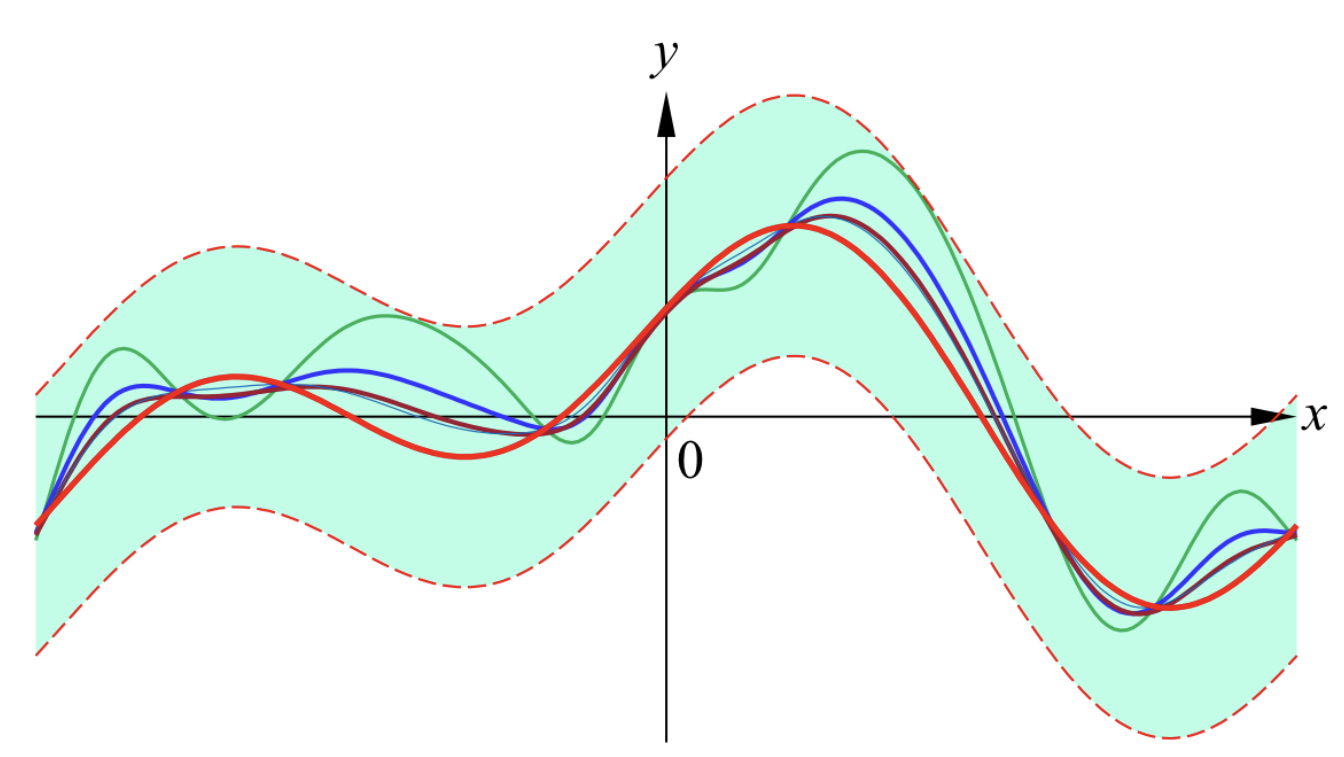
\includegraphics[scale=0.2]{Picture57.png}
\caption{Uniform convergence of a sequence of functions.\fa}\label{figure57}
\end{figure}


Obviously,  we have the following.
\begin{proposition}{}
Let $D$ be a subset of real numbers. If  $\{f_n:D\to\mathbb{R}\}$ is a sequence of functions that converges uniformly to the function $f:D\to\mathbb{R}$, then the sequence $\{f_n:D\to\mathbb{R}\}$  converges pointwise to  $f:D\to\mathbb{R}$.
\end{proposition}
\begin{highlight}{Uniform Limit and Pointwise Limit}
If a sequence of functions $\{f_n:D\to\mathbb{R}\}$  converges uniformly, the uniform limit is the same as the pointwise limit.
\end{highlight}



Let us compare the definitions of pointwise  and uniform convergence using logical expressions.
\begin{highlight}{Pointwise Convergence versus Uniform Convergence}
\begin{enumerate}[$\bullet$\;\;]
\item
The sequence of functions $\{f_n:D\to\mathbb{R}\}$ converges pointwise to the function $f:D\to\mathbb{R}$.
\[\forall\;x\in D,\; \forall \varepsilon>0,\;\exists N\in\mathbb{Z}^+,\;\forall \,n\geq N,\;|f_n(x)-f(x)|<\varepsilon.\]
\item
The sequence of functions $\{f_n:D\to\mathbb{R}\}$ converges uniformly to the function $f:D\to\mathbb{R}$.
\[\forall \varepsilon>0,\;\exists N\in\mathbb{Z}^+,\;\forall\;x\in D,\; \forall \,n\geq N,\;|f_n(x)-f(x)|<\varepsilon.\]
\end{enumerate}
\end{highlight}
One sees that it is a matter of the ordering of the quantifiers, but it makes a significant difference when we interchange the orders of a universal quantifier with  a existential quantifier.

 One should also compare the definition of uniform convergence to uniform continuity that we discussed in Section \ref{sec2.5}. In both cases, the uniformity is with respect to the domain $D$.

Before looking at some examples, let us highlight the negation of uniform continuity.
\begin{highlight}{Non-Uniform Convergence}
In logical expressions, the sequence of functions $\{f_n:D\to\mathbb{R}\}$ does not converge uniformly to the function $f:D\to\mathbb{R}$ is expressed by
\begin{equation}\label{eq230303_1}\exists \,\varepsilon>0,\;\forall N\in\mathbb{Z}^+,\;\exists\;x\in D,\; \exists \,n\geq N,\;|f_n(x)-f(x)|\geq \varepsilon.\end{equation}
\end{highlight}

The following gives a prelimary test for uniform convergence.
\begin{proposition}{}
If a sequence of functions $\{f_n:D\to\mathbb{R}\}$ does not converge pointwise, then it does not converge uniformly. 
\end{proposition}
If the sequence $\{f_n:D\to\mathbb{R}\}$ does converge pointwise, to show that it does not converge uniformly, we only need to establish the statement \eqref{eq230303_1} with $f:D\to\mathbb{R}$ the pointwise limit of the  sequence $\{f_n:D\to\mathbb{R}\}$.


\begin{example}[label=230303_7]{}For $n\geq 1$, let $f_n:[0,1]\to\mathbb{R}$ be the function $f_n(x)=x^n$.
Show that the sequence $\{f_n:[0,1]\to\mathbb{R} \}$ does not converge uniformly. 
\end{example}
\begin{solution}{Solution}In Example \ref{230303_1}, we have seen that the sequence $\{f_n \}$ converges  pointwise to the function $f:[0,1]\to\mathbb{R}$, where $f(x)=0$ for $x\in [0,1)$ and $f(1)=1$. If $\{f_n:[0,1]\to\mathbb{R}\}$  converges  uniformly, it must converge to the same function $f::[0,1]\to\mathbb{R}$. Take $\varepsilon=\frac{1}{2}$. There must be a positive integer $N$ such that for all $n\geq N$, for all $x\in [0,1]$,
\[|f_n(x)-f(x)|<\frac{1}{2}.\]\bs
In particular, this says that for all $x\in [0,1)$,
\[x^N<\frac{1}{2}.\]
This is absurd since $\di\lim_{x\to 1^-}x^N=1$. Hence, the  sequence $\{f_n:[0,1]\to\mathbb{R} \}$ does not converge uniformly. 
\end{solution}

\begin{example}[label=230303_8]{}For $n\geq 1$, let $f_n:\mathbb{R}\to\mathbb{R}$ be the function $f_n(x)=xe^{-nx^2}$.
Show that the sequence $\{f_n \}$  converges uniformly. 
\end{example}
\begin{solution}{Solution}In Example \ref{230303_4}, we have seen that the sequence $\{f_n\}$ converges pointwise to the function $f:\mathbb{R}\to\mathbb{R}$ that is identically 0.
Notice that 
\[f_n'(x)=(1-2nx^2)e^{-nx^2}.\]
This shows that $f'_n(x)>0$ for $|x|<1/\sqrt{2n}$, and $f'_n(x)<0$ for $|x|>1/\sqrt{2n}$. Since
\[\lim_{n\to-\infty}f_n(x)=0\quad\text{and}\quad\lim_{n\to\infty}f_n(x)=0,\]we find that $f_n(x)$  decreases from $0$ to $f_n(-1/\sqrt{2n})$ when $x$ goes from $-\infty$ to $ -1/\sqrt{2n}$, $f_n(x)$ increases from $f_n(-1/\sqrt{2n})$  to $f_n(1/\sqrt{2n})$ when $x$ goes from $-1/\sqrt{2n}$ to $1/\sqrt{2n}$, and $f_n(x)$ decreases from $f_n(1/\sqrt{2n})$ to 0 when $x$ goes from $1/\sqrt{2n}$ to $\infty$. Hence, the minimum and maximum values of $f_n$ are  $f_n(-1/\sqrt{2n})$ and $f_n(1/\sqrt{2n})$ respectively.
This shows that
\[|f_n(x)|\leq f_n(1/\sqrt{2n})=\frac{1}{\sqrt{2n}}e^{-\frac{1}{2}}\leq \frac{1}{\sqrt{2n}}\hspace{1cm}\text{for all}\;x\in\mathbb{R}.\]

Given $\varepsilon>0$, there is a positive integer $N$ such that $1/\sqrt{2N}<\varepsilon$. For all $n\in N$, for all $x\in\mathbb{R}$, we find that
\bs
\[|f_n(x)-f(x)|=|f_n(x)|\leq \frac{1}{\sqrt{2n}}\leq\frac{1}{\sqrt{2N}}<\varepsilon.\]
This proves that  the sequence of functions $\{f_n\}$ converges uniformly to the function $f$ that is identically 0.

\end{solution}

 By definition, if a sequence of functions $\{f_n:D\to\mathbb{R}\}$ converges uniformly to the function $f:D\to\mathbb{R}$, then there is a positive integer $N_0$ such that for all $n\geq N_0$, 
\[|f_n(x)-f(x)|<1\hspace{1cm}\text{for all}\;x\in D.\]
This implies that for all $n\geq N_0$, the function $(f_n-f):D\to\mathbb{R}$ is bounded above, and thus $\di M_n=\sup_{x\in D}|f_n(x)-f(x)|$ exists. 

The following theorem provides a systematic way to determine whether a sequence of functions $\{f_n:D\to\mathbb{R}\}$ converges uniformly.
\begin{theorem}[label=230303_9]{}
Let $D$ be a subset of real numbers, and let $\{f_n:D\to\mathbb{R}\}$ be a sequence of functions defined on $D$.
\begin{enumerate}[I.]
\item
If the sequence of functions $\{f_n:D\to\mathbb{R}\}$ does not converge pointwise to a function, then it does not converge uniformly.
\item If the sequence of functions $\{f_n:D\to\mathbb{R}\}$  converges pointwise to a function $f:D\to\mathbb{R}$, for each $n\in\mathbb{Z}^+$, define the function $g_n:D\to\mathbb{R}$ by $g_n(x)=f_n(x)-f(x)$.
\begin{enumerate}[(a)]
\item
If $g_n$ is not bounded for infinitely many $n$, then  the sequence of functions $\{f_n:D\to\mathbb{R}\}$ does not converge uniformly.
\item If only finitely many of the functions $g_n$ are not bounded, there is a positive integer $N_0$ such that $g_n$ is bounded for all $n\geq N_0$. For $n\geq N_0$, let $\di M_n=\sup_{x\in D}|g_n(x)|$. Then the  sequence of functions $\{f_n:D\to\mathbb{R}\}$  converges uniformly to the function $f:D\to\mathbb{R}$ if and only if $\di\lim_{n\to\infty}M_n=0$.
\end{enumerate}
\end{enumerate}
\end{theorem}
\begin{myproof}{Proof}
We have addressed I. and II. (a). Let us now consider II. (b). If the    sequence of functions $\{f_n:D\to\mathbb{R}\}$  converges uniformly to the function $f:D\to\mathbb{R}$, given $\varepsilon>0$, there is a positive integer $N\geq N_0$ such that for all $n\geq N$ and for all $x\in D$,
\[|g_n(x)|=|f_n(x)-f(x)|<\frac{\varepsilon}{2}.\]
This gives 
\[0\leq M_n=\sup_{x\in D}|g_n(x)|\leq\frac{\varepsilon}{2}<\varepsilon\hspace{1cm}\text{for all}\;n\geq N.\]
Therefore, $\di\lim_{n\to\infty}M_n=0$.
 
Conversely, if $\di\lim_{n\to\infty}M_n=0$, given $\varepsilon>0$, there is a positive integer $N\geq N_0$ such that 
\[M_n<\varepsilon\hspace{1cm}\text{for all}\;n\geq N.\]
It follows that for all $n\geq N$, for all $x\in D$,
\[|f_n(x)-f(x)|=|g_n(x)|\leq\sup_{x\in D}|g_n(x)|=M_n<\varepsilon.\]
This proves that the    sequence of functions $\{f_n:D\to\mathbb{R}\}$  converges uniformly to the function $f:D\to\mathbb{R}$.
\end{myproof}
\begin{example}{}
For  the sequence of functions discussed in Example \ref{230303_7}, \[f_n(x)-f(x)=\begin{cases}x^n,\quad &\text{if}\;0\leq x<1,\\0,\quad &\text{if}\;\quad x=1.\end{cases}\]Therefore,
\[M_n=\sup_{0\leq x\leq 1}|f_n(x)-f(x)|= 1.\]
Since $\di\lim_{n\to\infty}M_n=1\neq 0$,  Theorem \ref{230303_9} implies that the sequence of functions $\{f_n:[0,1]\to\mathbb{R}\}$ with $f_n(x)=x^n$ does not converge uniformly.
\end{example}

\begin{example}{}
For  the sequence of functions discussed in Example \ref{230303_8}, $f_n(x)-f(x)=f_n(x)=xe^{-nx^2}$. We have shown that
\[M_n=\sup_{x\in\mathbb{R}}|f_n(x)-f(x)|\leq\frac{ 1}{\sqrt{2n}}.\]
This implies that $\di\lim_{n\to\infty}M_n= 0$. Hence,  Theorem \ref{230303_9}  says that the sequence of functions $\{f_n:\mathbb{R}\to\mathbb{R}\}$ with $f_n(x)=xe^{-nx^2}$   converges uniformly.
\end{example}

To apply Theorem \ref{230303_9}, we need to know \emph{apriori} the pointwise limit of the sequence of functions $\{f_n\}$ to be able to conclude the uniform convergence of the sequence. Sometimes it could be difficult to find the limit function. To circumvent this problem, we introduce the concept of uniformly Cauchy.

\begin{definition}
{Uniformly Cauchy Sequence of Functions}Let $D$ be a subset of real numbers.
A sequence of functions $\{f_n:D\to\mathbb{R}\}$ is {\bf uniformly Cauchy} provided that for every $\varepsilon>0$, there is a positive integer $N$ such that for all $m\geq n\geq N$,
\[|f_m(x)-f_n(x)|<\varepsilon\hspace{1cm}\text{for all}\;x\in D.\]

\end{definition}
We have the following.
\begin{theorem}[label=230303_10]{~\\Cauchy Criterion for Uniform Convergence of Sequences of Functions}A sequence of functions $\{f_n:D\to\mathbb{R}\}$ converges uniformly if and only if it is uniformly Cauchy.
\end{theorem}
\begin{myproof}{Proof}
If the sequence of functions $\{f_n:D\to\mathbb{R}\}$ converges uniformly to $f:D\to\mathbb{R}$, given $\varepsilon>0$, there is a positive integer $N$ such that for all $n\geq N$,
\[|f_n(x)-f(x)|<\frac{\varepsilon}{2}\hspace{1cm}\text{for all}\;x\in D.\]
\bp
Using triangle inequality, this proves that for all $m\geq n\geq N$,
\[|f_m(x)-f_n(x)|<\varepsilon\hspace{1cm}\text{for all}\;x\in D.\]This proves that the sequence   $\{f_n:D\to\mathbb{R}\}$ is  uniformly Cauchy.


Conversely, if the sequence of functions $\{f_n:D\to\mathbb{R}\}$ is  uniformly Cauchy, then for each $x\in D$, the sequence $\{f_n(x)\}$ is a Cauchy sequence. Hence, it converges to a number $f(x)$. This shows that the sequence of functions $\{f_n:D\to\mathbb{R}\}$ converges pointwise to a function $f:D\to\mathbb{R}$. To show that the convergence is uniform, given $\varepsilon>0$, there is a positive integer $N$ such that for all $m\geq n\geq N$, 
\[|f_m(x)-f_n(x)|<\frac{\varepsilon}{2}\hspace{1cm}\text{for all}\;x\in D.\]   For each $x\in D$,  fixed $n\geq N$ and take the limit $m\to\infty$, we find that
\[|f_n(x)-f(x)|\leq\frac{\varepsilon}{2}.\]
This proves that for all $n\geq N$, for all $x\in D$, \[|f_n(x)-f(x)|<\varepsilon.\]Therefore, the sequence of functions $\{f_n:D\to\mathbb{R}\}$ converges uniformly.
\end{myproof}

Using Theorem \ref{230303_10},
Theorem \ref{230303_9} can be finetuned as follows. The proof is straightforward and we leave it to the exercises.
\begin{theorem}[label=230303_11]{}
Given that $\{f_n:D\to\mathbb{R}\}$ is a sequence of functions defined on the subset $D$ of real numbers, for each pair of $(m,n)\in\mathbb{Z}^+\times\mathbb{Z}^+$, define the extended real number $M_{m,n}$ as
\[M_{m,n}=\sup_{x\in D}|f_m(x)-f_n(x)|.\]Then the sequence of functions  $\{f_n:D\to\mathbb{R}\}$ converges uniformly if and only if the double sequence $\{M_{m,n}\}$ converges to 0.
\end{theorem}


Next we turn to series of functions.
\begin{definition}{Uniform Convergence of Series of Functions}
Let $D$ be a subset of real numbers and let $\{f_n:D\to\mathbb{R}\}$ be a sequence of functions defined on $D$. We say that  the series of functions $\di\sum_{n=1}^{\infty}f_n(x)$  converges uniformly to the function $s:D\to\mathbb{R}$ provided that the sequence of partial sums $\di\{s_n:D\rightarrow\mathbb{R}\}$ with $\di s_n(x)=\sum_{k=1}^nf_k(x)$ converges uniformly to the function $s(x)$.
 
\end{definition}

\begin{highlight}{Uniform Convergence of Series of Functions}A necessary condition for a series of functions to converge uniformly is that it converges pointwise.

When the series of functions  $\di\sum_{n=1}^{\infty}f_n(x)$ converges pointwise to a function $s(x)$ on a set $D$, then for any  $n\in \mathbb{Z}^+$ and any $x\in D$, the series
\[\sum_{k=n}^{\infty}f_k(x)\] converges pointwise to the function $s(x)-s_{n-1}(x)$, where  $\di s_n(x)=\sum_{k=1}^nf_k(x)$ is the $n^{\text{th}}$ partial sum, and $s_0(x)=0$ by default.

Therefore, we can reformulate the definition of uniform convergence of series of functions as follows.   The series $\di\sum_{n=1}^{\infty}f_n(x)$  converges uniformly to the function $s(x)$ on the set $D$ provided that for any $\varepsilon>0$, there is a positive integer $N$ such that for all $n\geq N$, 
\[\left|\sum_{k=n}^{\infty} f_k(x)\right|<\varepsilon\hspace{1cm}\text{for all}\;x\in D.\]
\end{highlight}

In most cases, such as Example \ref{230304_4}, we can only justify a series of functions converges pointwise, but we cannot find an explicit close form for the sum $s(x)$. In this case, a Cauchy criterion becomes useful.

From Theorem \ref{230303_10}, we obtain the following immediately. 
\begin{theorem}[label=230304_7]{~\\Cauchy Criterion for Uniform Convergence of Series of Functions}A series of functions $\di\sum_{n=1}^{\infty}f_n(x)$ converges uniformly on a set $D$ if and only if for every $\varepsilon>0$, there is a positive integer $N$ such that for all $m\geq n\geq N$,
\[\left|\sum_{k=n}^mf_k(x)\right|<\varepsilon\hspace{1cm}\text{for all}\;x\in D.\]
\end{theorem}

\begin{example}[label=230304_9]{}
For the series $\di\sum_{n=1}^{\infty}e^{-n^2x}$ considered in Example \ref{230304_4}, we have shown that it converges pointwise on the interval $(0,\infty)$. Let us prove that the convergence is uniform on any set $D$ of the form $D=[a, \infty)$, where $a$ is a positive constant.

We notice that if $m\geq n$ and $x\geq a$,
\[0\leq \sum_{k=n}^me^{-k^2x}\leq\sum_{k=n}^me^{-kx}\leq\sum_{k=n}^{\infty}e^{-kx}\leq \sum_{k=n}^{\infty}e^{-ka}= \frac{e^{-na}}{1-e^{-a}}.
\]
Given $\varepsilon>0$, since \[\lim_{n\to\infty}\frac{e^{-na}}{1-e^{-a}}=0,\]there exists a positive integer $N$ such that for all $n\geq N$,
\[0\leq \frac{e^{-na}}{1-e^{-a}}<\varepsilon.\]\be
It follows that for all $m\geq n\geq N$, and for all $x\in[a,\infty)$,
\[\left|\sum_{k=n}^me^{-k^2x}\right|\leq \frac{e^{-na}}{1-e^{-a}}<\varepsilon.\]
By Theorem \ref{230304_7}, the series $\di\sum_{n=1}^{\infty}e^{-n^2x}$ converges uniformly on $[a, \infty)$.
\end{example2}
The readers are invited  to show that the series $\di\sum_{n=1}^{\infty}e^{-n^2x}$ does not converge uniformly on the set $(0,\infty)$. 
It is  a typical situation that allthough the series converges pointwise on a set $A$,   it fails to converge uniformly on $A$, but it converges uniformly on  subsets of $A$. Most of the time, we do not need uniform convergence on $A$, but uniform convergence on a collection of subsets of $A$ whose union  is $A$ is enough. In the example above, $\mathscr{C}=\left\{[a, \infty)\,|\, a\geq 0\right\}$ is a collection of subsets of $A=(0,\infty)$ whose union is $A$. 

\begin{definition}{Absolute  Convergence of Series of Functions}
 A series of  functions $\di\sum_{n=1}^{\infty}f_n(x)$ is said to converge absolutely on a set $D$ if the series $\di\sum_{n=1}^{\infty}|f_n(x)|$ converges pointwise on $D$. In this case, the series $\di\sum_{n=1}^{\infty}f_n(x)$ also converges pointwise on $D$.  
\end{definition}

Now we   present a useful test to show that a series of functions converges absolutely and uniformly on a set $D$.
\begin{theorem}[label=230617_1]{}Let $\{f_n:D\to \mathbb{R}\}$ be a sequence of functions defined on $D$. If the series
 $\di\sum_{n=1}^{\infty}|f_n(x)|$ converges uniformly on $D$, then the series $\di\sum_{n=1}^{\infty}f_n(x)$ converges absolutely and  uniformly on $D$.
\end{theorem}
\begin{myproof}{Proof}
Since  the series
 $\di\sum_{n=1}^{\infty}|f_n(x)|$ converges uniformly on $D$, it also converges pointwise. Hence, the series $\di\sum_{n=1}^{\infty}f_n(x)$ converges absolutely on $D$.
 
Since   $\di\sum_{n=1}^{\infty}|f_n(x)|$ converges uniformly on $D$, it is uniformly Cauchy. Given $\varepsilon>0$, there is a positive integer $N$ such that for all $m\geq n\geq N$,
\[\sum_{k=n}^m|f_k(x)|<\varepsilon \hspace{1cm}\text{for all}\;x\in D.\]
Triangle inequality implies that
\[\left|\sum_{k=n}^mf_k(x)\right|\leq \sum_{k=n}^m|f_k(x)|<\varepsilon \hspace{1cm}\text{for all}\;x\in D.\]
 
Hence, the series $\di\sum_{n=1}^{\infty}f_n(x)$ is also uniformly Cauchy on $D$. Therefore, it also converges uniformly.
\end{myproof}
\begin{theorem}[label=230305_8]{Weiertrass M-Test}
Let $\{f_n:D\to \mathbb{R}\}$ be a sequence of functions defined on $D$. Assume that the following conditions are satisfied.
\begin{enumerate}[(i)]
\item
For each $n\in\mathbb{Z}^+$, there is a positive constant $M_n$ such that $|f_n(x)|\leq M_n$ for all $x\in D$.
\item The series $\di\sum_{n=1}^{\infty}M_n$ is convergent.
\end{enumerate}Then the series $\di\sum_{n=1}^{\infty}f_n(x)$ converges absolutely and uniformly on $D$. 
\end{theorem}
\begin{myproof}{Proof}By Theorem \ref{230617_1}, we only
 need to show that the series $\di\sum_{n=1}^{\infty}|f_n(x)|$ converges uniformly on $D$.
Given $\varepsilon>0$, since the series $\di\sum_{n=1}^{\infty}M_n$ is convergent, there is a positive integer $N$ such that for all $m\geq n\geq N$,
\[ \sum_{k=n}^m M_k<\varepsilon.\]This implies that
\[\sum_{k=n}^m|f_k(x)|\leq\sum_{k=n}^mM_k<\varepsilon\hspace{1cm}\text{for all}\;x\in D.\]
By Theorem \ref{230304_7}, the series  $\di\sum_{n=1}^{\infty}|f_n(x)|$ converges uniformly on $D$.
\end{myproof}

\begin{example}{}
Let $a$ be a positive number. Show that the series  $\di\sum_{n=1}^{\infty}(-1)^{n-1}e^{-n^2x}$ converges absolutely and  uniformly on $[a,\infty)$.  
\end{example}
\begin{solution}{Solution}
For $n\in\mathbb{Z}^+$, let $f_n(x)=\di (-1)^{n-1}e^{-n^2x}$. For $x\in [a, \infty)$, $x\geq a$. Hence, for $n\in\mathbb{Z}^+$,
\[|f_n(x)|=e^{-n^2x}\leq e^{-nx}\leq e^{-na}.\]
Since $r=e^{-na}<1$, the geometric series $\di\sum_{n=1}^{\infty} e^{-na}$ is convergent. By Weierstrass $M$-test, the series $\di\sum_{n=1}^{\infty}(-1)^{n-1}e^{-n^2x}$ converges absolutely and  uniformly on $[a,\infty)$. 
\end{solution}

\vp
\noindent
{\bf \large Exercises  \thesection}
\setcounter{myquestion}{1}
\begin{question}{\themyquestion}
For $n\geq 1$, let $f_n:[0,1]\to\mathbb{R}$ be the function $f_n(x)=e^{-nx^2}$.
Show that the sequence of functions $\{f_n \}$ does not converge uniformly. 
\end{question}
\atc
\begin{question}{\themyquestion}
For $n\geq 1$, let $f_n:\mathbb{R}\to\mathbb{R}$ be the function $\di f_n(x)=n\sin\left(\frac{x}{n}\right)$. Show that the sequence of functions $\{f_n \}$  does not converge uniformly. 
\end{question}

\atc
\begin{question}{\themyquestion}
For $n\geq 1$, let $f_n:[0,2\pi]\to\mathbb{R}$ be the function $\di f_n(x)=n\sin\left(\frac{x}{n}\right)$. Show that the sequence of functions $\{f_n \}$  converges uniformly. 
\end{question}
\atc
\begin{question}{\themyquestion}
For $n\geq 1$, let $f_n:[0,\infty)\to\mathbb{R}$ be the function $\di f_n(x)=\frac{x}{1+nx}$. Determine whether the sequence of functions $\{f_n \}$  converges uniformly. 
\end{question}
 
 \atc
\begin{question}{\themyquestion}
Let $a$ be a positive constant. Show that the series $\di\sum_{n=1}^{\infty}(-1)^{n-1}ne^{-n^2x}$ converges absolutely and uniformly on the set $[a, \infty)$.
\end{question}
\vp
\section{Properties of  Uniform Limits of Functions}\label{sec6.3}

In this section, we are going to see how uniform convergence can avoid the pathological behaviours we mentioned in the beginning of Section \ref{sec6.2}. First we show that uniform limit of continuous functions is continuous. This is a very important result in mathematical analysis.
\begin{theorem}[label=230304_1]{Uniform Limit of Continuous Functions is Continuous}
Given that $D$ is a subset of real numbers, and $\{f_n:D\to\mathbb{R}\}$ is a sequence of continuous functions that converges uniformly to the function $f:D\to\mathbb{R}$. Then the function  $f:D\to\mathbb{R}$ is continuous. 
\end{theorem}\begin{myproof}{Proof}
The proof is a standard $1/3$ argument. Given $x_0\in D$, we want to show that $f$ is continuous at $x_0$ using the $\varepsilon-\delta$ argument. Given $\varepsilon>0$, there is a positive integer $N$ such that for all $n\geq N$, 
\[|f_n(x)-f(x)|<\frac{\varepsilon}{3}\hspace{1cm}\text{for all}\;x\in D.\]We are only going to use this statement when $n=N$.
Since $f_N$ is continuous at $x_0$, there is a $\delta>0$ such that for all $x\in D$, if $|x-x_0|<\delta$, then
\[|f_N(x)-f_N(x_0)|<\frac{\varepsilon}{3}.\]

From these, we find that if $x$ is in $D$ and $|x-x_0|<\delta$, then
\begin{align*}
|f(x)-f(x_0)|&\leq |f(x)-f_N(x)|+|f_N(x)-f_N(x_0)|+|f_N(x_0)-f(x_0)|\\&<\frac{\varepsilon}{3}+\frac{\varepsilon}{3}+\frac{\varepsilon}{3}=\varepsilon.\end{align*}This proves that $f$ is continuous at $x_0$.
 
\end{myproof}
\begin{example}{}
 For the sequence of functions $\{f_n:[0,1]\to\mathbb{R}\}$ with $f_n(x)=x^n$, its pointwise limit $f:[0,1]\to\mathbb{R}$,  \[f(x)=\begin{cases}0,\quad &\text{if}\;x\neq 0,\\1,\quad &\text{if}\; x=0,\end{cases}\]
is  not continuous. Since  each $f_n$, $n\in\mathbb{Z}^+$ is a continuous function,
  Theorem \ref{230304_1} can be used to infer that the sequence of functions  $\{f_n:[0,1]\to\mathbb{R}\}$ with $f_n(x)=x^n$  does not converge uniformly.  

 
\end{example}
Applying Theorem \ref{230304_1} to series of functions, we have the following.
\begin{corollary}[label=230305_10]{}
Given that $\{f_n:D\rightarrow \mathbb{R}\}$ is a sequence of continuous functions defined on $D$. If the series of functions $\di\sum_{n=1}^{\infty}f_n(x)$ converges uniformly on  $D$, then it defines a continuous function $s:D\to\mathbb{R}$ by
\[s(x)=\sum_{n=1}^{\infty}f_n(x).\]
\end{corollary}\begin{myproof}{Proof}
We apply  Theorem \ref{230304_1} to the sequence of partial sums $\{s_n(x)\}$. Since $\di s_n(x)=\di\sum_{k=1}^nf_k(x)$ is a finite sum of continuous functions, it is continuous. By Theorem \ref{230304_1}, $\di s(x)=\lim_{n\to\infty}s_n(x)$ is continuous.
\end{myproof}

Next, we turn to integration.
\begin{theorem}[label=230304_2]{}
 Assume that for  each $n\in\mathbb{Z}^+$, the funtion $f_n:[a,b]\to\mathbb{R}$ is Riemann integrable. If the sequence of functions $\{f_n:[a,b]\to\mathbb{R}\}$   converges uniformly to the function $f:[a,b]\to\mathbb{R}$, then $f:[a,b]\to\mathbb{R}$ is also Riemann integrable, and the orders of the limit operation and the integration operation can be interchanged. Namely,
\begin{equation}\label{eq230304_3}
\lim_{n\to\infty}\int_a^b f_n(x)dx=\int_a^bf(x)dx=\int_a^b\lim_{n\to\infty}f_n(x)dx.
\end{equation}
\end{theorem}
Notice that we only assume that each $f_n$ is Riemann integrable. We do not need to assume that it is continuous.
\begin{myproof}{Proof}
Given $\varepsilon>0$, there is a positive integer $N$ such that for all $n\geq N$, 
\begin{equation}\label{eq230304_5}|f_n(x)-f(x)|<\frac{\varepsilon}{3(b-a)}\hspace{1cm}\text{for all}\;x\in [a,b].\end{equation} First we take $n=N$. Since $f_N:[a,b]\to\mathbb{R}$ is Riemann integrable, there is a partition  $P=\{x_i\}_{i=0}^k$  of $[a,b]$ such that
\[U(f_N,P)-L(f_N,P)<\frac{\varepsilon}{3}.\]From \eqref{eq230304_5}, we have
\[f_N(x)-\frac{\varepsilon}{3(b-a)}<f(x)<f_N(x)+\frac{\varepsilon}{3(b-a)}\hspace{1cm}\text{for all}\;x\in [a,b].\]
  For any $1\leq i\leq k$, if $x\in [x_{i-1}, x_i]$,
\begin{align*}
\inf_{x_{i-1}\leq x\leq x_i}f_N(x)-\frac{\varepsilon}{3(b-a)}\leq f(x)\leq \sup_{x_{i-1}\leq x\leq x_i}f_N(x)+\frac{\varepsilon}{3(b-a)}.
\end{align*}This implies that
\begin{align*}\inf_{x_{i-1}\leq x\leq x_i}f_N(x)&-\frac{\varepsilon}{3(b-a)} \leq \inf_{x_{i-1}\leq x\leq x_i}f(x)\\ &\leq  \sup_{x_{i-1}\leq x\leq x_i}f(x)\leq \sup_{x_{i-1}\leq x\leq x_i}f_N(x)+\frac{\varepsilon}{3(b-a)}.\end{align*}
 \bp
Therefore,
\[U(f,P)\leq U(f_N,P)+\frac{\varepsilon}{3},\hspace{1cm}L(f,P)\geq L(f_N,P)-\frac{\varepsilon}{3}.\] 
Thus,
\[U(f,P)-L(f,P)\leq U(f_N,P)-L(f_N,P)+\frac{2\varepsilon}{3}<\frac{\varepsilon}{3}+\frac{2\varepsilon}{3}=\varepsilon.\]
From this, we conclude  that $f$ is Riemann integrable.
 This in turn implies that for any $n\in\mathbb{Z}^+$, the function $f_n-f$ is Riemann integrable on $[a,b]$, and so is the function $|f_n-f|$.
With the same $\varepsilon>0$, we find from \eqref{eq230304_5} that for any $n\geq N$,
\begin{align*}
\left|\int_a^bf_n(x)dx-\int_a^b f(x)dx\right|&=\left|\int_a^b(f_n(x)-f(x))dx\right|\\&\leq \int_a^b\left|f_n(x)-f(x) \right|dx\leq \frac{\varepsilon}{3}<\varepsilon.
\end{align*}This proves that \eqref{eq230304_3} holds.
 
\end{myproof}

Applying Theorem \ref{230304_2} to series of functions, we have the following.
\begin{corollary}[label=230305_11]{}
Given that $\{f_n:[a,b]\rightarrow \mathbb{R}\}$ is a sequence of Riemann integrable functions. If the series $\di\sum_{n=1}^{\infty}f_n(x)$ converges uniformly, then the function $\di s(x)=\sum_{n=1}^{\infty}f_n(x)$ is Riemann integrable, the series $\di \sum_{n=1}^{\infty}\int_a^bf_n(x)dx$ is convergent, and we can integrate term by term. Namely,
\[\int_a^bs(x)dx=\int_a^b \sum_{n=1}^{\infty}f_n(x)dx=\sum_{n=1}^{\infty}\int_a^bf_n(x)dx.\] 
\end{corollary}
\begin{myproof}{Proof}
We apply  Theorem \ref{230304_2} to the sequence of partial sums $\{s_n(x)\}$. Since $\di s_n(x)=\di\sum_{k=1}^nf_k(x)$ is a finite sum of Riemann integrable functions, it is Riemann integrable. The rest follows from Theorem \ref{230304_2}.
\end{myproof}
\begin{example}{}
In Example \ref{230303_6}, the sequence of functions $\{f_n:[0,1]\to\mathbb{R}\}$ converges pointwise to the function $f:[0,1]\to\mathbb{R}$ that is identically 0. However, since
$\di\int_0^1f_n(x)dx=1/6$, the sequence $\di\left\{\int_0^1f_n(x)dx\right\}$ does not converge to $\di\int_0^1f(x)dx=0$. Theorem \ref{230304_2} can be used to deduce that $\{f_n:[0,1]\to\mathbb{R}\}$ does not converge to $f:[0,1]\to\mathbb{R}$ uniformly. 

In fact, one can verify that 
\[M_n=\sup_{0\leq x\leq 1}|f_n(x)-f(x)|=\sup_{0\leq x\leq 1/n}n^2x\left(1-nx\right)=\frac{n}{4}.\]Since $\di\lim_{n\to\infty}M_n\neq 0$,    $\{f_n:[0,1]\to\mathbb{R}\}$ does not converge to $f:[0,1]\to\mathbb{R}$ uniformly. 
\end{example}



Now we consider differentiation. In Example \ref{230303_8}, we have shown that the sequence $\{f_n:\mathbb{R}\to\mathbb{R}\}$ defined by $f_n(x)=xe^{-nx^2}$ converges uniformly to the function $f:\mathbb{R}\to\mathbb{R}$ that is identically zero. In Example \ref{230303_4}, we have seen that the derivative sequence $\{f_n'\}$ converges to the function $g:\mathbb{R}\to\mathbb{R}$ given  by
\[g(x)=\begin{cases}0,\quad &\text{if}\;x\neq 0,\\1,\quad &\text{if}\; x=0,\end{cases}\]We  find that
\[\left.\frac{d}{dx} \right|_{x=0}\lim_{n\to\infty} f_n(x)=0 \quad\text{which is not equal to}\quad\lim_{n\to\infty} \left.\frac{d}{dx} \right|_{x=0}f_n(x)=1.\]
Hence, even though the seqeunce of functions $\{f_n\}$ converges uniformly, we cannot interchange limit with differentiation.

 The following theorem gives a sufficient condition for interchanging limit with differentiation.



 
\begin{theorem}[label=230304_8]{}
Given that   $\{f_n:(a,b)\to\mathbb{R}\}$ is a sequence of   functions which satisfies the following conditions.
\begin{enumerate}[(i)]
\item There is a point $x_0$ in the interval $(a,b)$ such that the sequence   $\{f_n(x_0)\}$ converges to a number   $y_0$.
\item For each $n\in\mathbb{Z}^+$, $f_n:(a,b)\to\mathbb{R}$ is   differentiable.
\item The sequence of derivative functions $\{f_n':(a,b)\to\mathbb{R}\}$ converges uniformly to a function $g:(a,b)\to\mathbb{R}$.

\end{enumerate}
Then we have the following.
\begin{enumerate}[(a)]
\item The sequence of functions $\{f_n:(a,b)\to\mathbb{R}\}$ converges uniformly to a function $f:(a,b)\to\mathbb{R}$.
\item The function $f:(a,b)\to\mathbb{R}$ is differentiable.
\item  We can interchange differentiation and limits. Namely, for any $x\in (a,b)$, \[f'(x)= \frac{d}{dx}\lim_{n\to\infty}f_n(x)=\lim_{n\to\infty}\frac{d}{dx}f_n(x)= g(x).\]
\end{enumerate}
\end{theorem}
 

\begin{myproof}{Proof}For each $n\in\mathbb{Z}^+$,  since $f_n:I\to\mathbb{R}$ is   differentiable, it is continuous.
Given a point $c$ in the interval $(a,b)$, let $\{h_{n,c}:(a,b)\to\mathbb{R}\}$ be a sequence of functions defined by
\begin{equation}\label{eq230304_13}h_{n,c}(x)=\begin{cases} \di\frac{f_n(x)-f_n(c)}{x-c},\quad &\text{if}\;x\neq c,\\f_n'(c),\quad &\text{if}\;x=c.\end{cases}\end{equation}\bp
Then $h_{n,c}:(a,b)\to\mathbb{R}$ is a continuous function. 
For any positive integers $m$ and $n$, we have
\[h_{m,c}(x)-h_{n,c}(x)=\begin{cases} \di\frac{(f_m(x)-f_n(x))-(f_m(c)-f_n(c))}{x-c},\quad &\text{if}\;x\neq c,\\f_m'(c)-f_n'(c),\quad &\text{if}\;x=c.\end{cases}\]
Applying  mean value theorem to the differentiable function $f_m(x)-f_n(x)$, we find that  for any $x\in (a,b)\setminus\{c\}$, there is a point $\xi_x$ in between $x$ and $c$ such that
\[h_{n,c}(x)= f_{m}'(\xi_x)-f_n'(\xi_{x}).\]

Thus, we find that for any $x\in (a,b)$,
\[|h_{m,c}(x)-h_{n,c}(x)|\leq \sup_{a<x<b}|f_m'(x)-f_n'(x)|.\]
This implies that
\begin{equation}\label{eq230304_10}\sup_{a<x<b}|h_{m,c}(x)-h_{n,c}(x)|\leq \sup_{a<x<b}|f_m'(x)-f_n'(x)|.\end{equation}
Since the sequence of functions $\{f_n'\}$ converges uniformly, Theorem \ref{230303_11} implies that
\[\lim_{m,n\to\infty} \sup_{a<x<b}|f_m'(x)-f_n'(x)|=0.\]
Eq. \eqref{eq230304_10} then implies that 
\[\lim_{m,n\to\infty} \sup_{a<x<b}|h_{m,c}(x)-h_{n,c}(x)|=0.\]
By Theorem  \ref{230303_11} again, we find that the sequence of functions $\{h_{n,c}:(a,b)\to\mathbb{R}\}$ converges uniformly.

Now we specialize to $c=x_0$. Notice that by definition, 
\begin{equation}
\label{eq230304_12} f_m(x)-f_n(x)=f_m(x_0)-f_n(x_0)+(x-x_0)\left(h_{m,x_0}(x)-h_{n,x_0}(x)\right).\end{equation}Given $\varepsilon>0$, since the sequence $\{f_n(x_0)\}$ is convergent, there is a positive integer $N_1$ such that for all $m\geq n\geq N_1$, 
\[|f_m(x_0)-f_n(x_0)|<\frac{\varepsilon}{2}.\]\bp
Since the sequence of functions $\{h_{n,x_0}(x)\}$ converges uniformly,   Theorem \ref{230303_10} implies that there is a positive integer $N\geq N_1$ such that for all $m\geq n\geq N$,
\[|h_{m,x_0}(x)-h_{n,x_0}(x)|<\frac{\varepsilon}{2(b-a)}\hspace{1cm}\text{for all}\;x\in (a,b).\]
Eq. \eqref{eq230304_12}   implies that for all $m\geq n\geq N$, and for all $x\in (a,b)$,
\begin{align*}
|f_m(x)-f_n(x)|&\leq |f_m(x_0)-f_n(x_0)|+|x-x_0||h_{m,x_0}(x)-h_{n,x_0}(x)|
\\
&<\frac{\varepsilon}{2}+(b-a)\times \frac{\varepsilon}{2(b-a)}=\varepsilon.
\end{align*}

By Theorem \ref{230303_10}, this proves that the sequence of functions $\{f_n:(a,b)\to\mathbb{R}\}$ converges uniformly.   Let
\[f(x)=\lim_{n\to \infty}f_n(x)\] be the limit function. Being the limit of a sequence of continuous functions that converges uniformly, Theorem \ref{230304_1} says hat the function $f:(a,b)\to\mathbb{R}$ is continuous. 

 Now we want to prove that $f$ is differentiable and $f'(x)=g(x)$ for each $x\in (a,b)$. 
For any fixed $c\in (a,b)$, since the sequence of continuous functions $\{h_{n,c}(x)\}$ converges uniformly, it also converges pointwise. Taking $n\to\infty$ limits  in \eqref{eq230304_13}, we find that
\[h_c(x)=\lim_{n\to \infty}h_{n,c}(x)=\begin{cases}\di\frac{f(x)-f(c)}{x-c}, \quad &\text{if}\;x\neq c,\\g(c),\quad &\text{if}\;x=c.\end{cases}.\]

Since $\{h_{n,c}(x)\}$ is a sequence of continuous functions that converges uniformly,  Theorem \ref{230304_1} says that the limit function $h_c:(a,b)\to\mathbb{R}$ is continuous. Therefore,
\[g(c)=h_c(c)=\lim_{x\to c}h_c(x)=\lim_{x\to c}\frac{f(x)-f(c)}{x-c}.\]
This shows that $f$ is differentiable at $x=c$ and $f'(c)=g(c)$.
\end{myproof}

\begin{remark}{}
 \begin{enumerate}[1.]
 \item 
 In   Theorem \ref{230304_8}, we do not need to assume that the sequence of functions $\{f_n\}$ converges uniformly. It is a consequence of uniform convergence of the sequence $\{f_n'\}$. The condition that there is a point $x_0$ in $(a,b)$ so that  the sequence   $\{f_n(x_0)\}$ converges is  necessary. For otherwise  if we let $\widetilde{f}_n(x)=f_n(x)+n$ for  $n\in\mathbb{Z}^+$, then $\widetilde{f}_n'(x)=f_n'(x) $. But the sequence $\{\widetilde{f}_n\}$ does not converge if the sequence $\{f_n\}$  is convergent.
 \item
If we assume that  for all $n\in\mathbb{Z}^+$, the function  $f_n:(a,b)\to\mathbb{R}$ is continuously differentiable, there is an easier proof for the conclusions in Theorem \ref{230304_8}. \end{enumerate}
\end{remark}

Applying Theorem \ref{230304_8} to series of functions, we have the following.
\begin{corollary}[label=230304_14]
{}Let $\{f_n:(a,b)\to\mathbb{R}\}$ be a sequence of differentiable functions. Assume that there is a  $x_0\in (a, b)$ such that the series $\di\sum_{n=1}^{\infty}f_n(x_0)$ is convergent, and the series $\di\sum_{n=1}^{\infty}f_n'(x)$ converges uniformly on $(a,b)$, then the series  $\di\sum_{n=1}^{\infty}f_n(x)$ converges uniformly on $(a,b)$ to a differentiable function whose derivative is given by
\[\frac{d}{dx}\sum_{n=1}^{\infty}f_n(x)=\sum_{n=1}^{\infty}f_n'(x)\hspace{1cm}\text{for all}\;x\in (a,b).\]
\end{corollary}
\begin{myproof}{Proof}
Applying Theorem \ref{230304_8} to the sequence of partial sums $\{s_n(x)\}$. Since $\di s_n(x)=\di\sum_{k=1}^nf_k(x)$ is a finite sum of differentiable functions, it is differentiable. The rest follows from Theorem \ref{230304_8}.
\end{myproof}

\begin{example}{}
Consider the series $\di\sum_{n=1}^{\infty} e^{-n^2x}$ discussed in Example \ref{230304_9}. We have shown that it converges uniformly on $[a,\infty)$ when $a$ is a positive number.  For each $n\in\mathbb{Z}^+$, $f_n(x)=\di-\frac{1}{n^2}e^{-n^2 x}$ is a differentiable function with derivative 
\[\frac{d}{dx}\left(-\frac{1}{n^2}e^{-n^2 x}\right)=e^{-n^2 x}.\]
Notice that  
\[|f_n(x)|\leq \frac{1}{n^2}\hspace{1cm}\text{for all}\;x\in [0,\infty).\]
 
Since the series $\di\sum_{n=1}^{\infty}\frac{1}{n^2}$ is convergent, 
 Weierstrass $M$-test shows that the series $\di \sum_{n=1}^{\infty} f_n(x)=\sum_{n=1}^{\infty}-\frac{1}{n^2}e^{-n^2x}$ converges absolutely and uniformly on $[0, \infty)$. Corollary \ref{230304_14} shows that for any $x\in (a, \infty)$, we can do term by term differentiation and obtain
 \begin{equation}\label{eq230304_11}\frac{d}{dx}\sum_{n=1}^{\infty}-\frac{1}{n^2}e^{-n^2x}=\sum_{n=1}^{\infty} e^{-n^2x}.\end{equation}
 Since $a>0$ is arbitrary, eq. \eqref{eq230304_11} holds for any $x>0$. However, this is not true for $x=0$ even if we only consider right derivatives, as the right hand side of the equation is divergent when $x=0$.
\end{example}



\vp
\noindent
{\bf \large Exercises  \thesection}
\setcounter{myquestion}{1}
\begin{question}{\themyquestion}
\begin{enumerate}[(a)]\item Show that 
the series $\di\sum_{n=1}^{\infty} n^2e^{-n^2x}$ defines a continuous function on $(0,\infty)$.
\item 
Show that 
the series $\di\sum_{n=1}^{\infty}  e^{-n^2x}$ defines a differentiable function on $(0,\infty)$, and for each $x>0$,
\[\frac{d}{dx}\sum_{n=1}^{\infty}  e^{-n^2x}=-\sum_{n=1}^{\infty} n^2e^{-n^2x}.\]\end{enumerate}
\end{question}
\atc
\begin{question}{\themyquestion}
 Let $\{f_n:(a,b)\to\mathbb{R}\}$ be a sequence of continuously differentiable  functions. Assume that there is a point $x_0\in [a,b]$ such that the sequence $\{f_n(x_0)\}$ converges to a point $y_0$, and the sequence of functions $\{f_n':(a,b)\to\mathbb{R}\}$ converges uniformly to a function $g:(a,b)\to\mathbb{R}$. Use the fundamental theorems of calculus and Theorem \ref{230304_2} to prove that the sequence of functions $\{f_n:(a,b)\to\mathbb{R}\}$ converges uniformly to a differentiable function $f:(a,b)\to\mathbb{R}$, and $f'(x)=g(x)$ for all $x\in (a,b)$.
\end{question}
 
\vp
\section{Power Series}\label{sec6.4}
In this section, we turn to consider a special class of series of functions  called {\it power series}. The partial sums of a power series are polynomial functions. Hence, power series are limits of polynomial sequences. They play important roles in analysis.
\begin{definition}{Power series}A power series in the variable $x$ is a series of the form
\[\sum_{n=0}^{\infty}c_n(x-x_0)^n,\]
where $x_0$ is a fixed real number, and $c_0, c_1, c_2, \ldots$ are the coefficients. 

\end{definition}
Each term in a power series $\di \sum_{n=0}^{\infty}c_n(x-x_0)^n$ is a simple polynomial $c_n(x-x_0)^n$ which is infinitely differentiable. However, as an infinite series, we need to address the convergence issue. Obviously, the power series $\di \sum_{n=0}^{\infty}c_n(x-x_0)^n$  converges when $x=x_0$. 

Recall that in Chapter \ref{ch5}, we have discussed the ratio test in Theorem \ref{230305_4}. Given $\di\sum_{n=1}^{\infty}a_n$ is a series with $a_n\neq 0$ for all $n\in\mathbb{Z}^+$, let
\[r=\liminf_{n\to\infty}\left|\frac{a_{n+1}}{a_n}\right|\hspace{1cm}\text{and}\hspace{1cm} R=\limsup_{n\to\infty}\left|\frac{a_{n+1}}{a_n}\right|.\]
Then the series $\di\sum_{n=1}^{\infty}a_n$  is divergent if $r>1$, convergent if $R<1$, but inconclusive if $r\leq 1\leq R$.
This test is useful if the limit $\di\lim_{n\to\infty}\left|\frac{a_{n+1}}{a_n}\right|$ exists. For then $r=R$ and we only left with finitely many points which we cannot conclude the convergence of the power series.
Let us look at some examples.
\begin{example}[label=230305_1]{}
Find the domain of convergence of the power series $\di \sum_{n=0}^{\infty}\frac{x^n}{n!}$.
\end{example}
\begin{solution}{Solution}
The power series is convergent when $x=0$. When $x\neq 0$,  using ratio test with $a_n=\di \frac{x^n}{n!}$, we find that
\[ \lim_{n\to\infty}\left|\frac{a_{n+1}}{a_n}\right|=\lim_{n\to\infty}\frac{|x|}{n+1}=0.\] 
Therefore, the series is convergent for all real numbers $x$. The domain of convergence is $\mathbb{R}$, the set of real numbers.
\end{solution}

\begin{example}[label=230305_2]{}
Find the domain of convergence of the power series $\di \sum_{n=0}^{\infty}n!x^n $.
\end{example}
\begin{solution}{Solution}
The power series is convergent when $x=0$. When $|x|\neq 0$, using ratio test with $a_n=\di  n!x^n$, we have 
\[ \lim_{n\to\infty}\left|\frac{a_{n+1}}{a_n}\right|=\lim_{n\to\infty}(n+1)|x|=\infty.\] Hence, the series is divergent if $x\neq 0$.
We conclude that the  series $\di \sum_{n=0}^{\infty}n!x^n $ is only convergent when $x=0$. The domain of convergence is the set $\{0\}$.
\end{solution}

\begin{example}[label=230305_3]{}
Find the domain of convergence of the power series $\di \sum_{n=1}^{\infty}\frac{x^n}{n^2}$.
\end{example}
\begin{solution}{Solution}
The power series is convergent when $x=0$. When $x\neq 0$,
  using  ratio test with $a_n=\di \frac{x^n}{n^2}$, we have
\[ \lim_{n\to\infty}\left|\frac{a_{n+1}}{a_n}\right|=|x|\lim_{n\to\infty}\frac{n^2}{(n+1)^2}=|x|\lim_{n\to\infty}\left(\frac{n}{n+1}\right)^2=|x|.\]
 

Therefore, the series is convergent if $|x|<1$, and divergent if $ |x|>1$. When $|x|=1$, the test is inconclusive.

But we know that the series $\di\sum_{n=1}^{\infty}\frac{1}{n^2}$ and the series $\di\sum_{n=1}^{\infty}\frac{(-1)^n}{n^2}$ are convergent. Therefore, the series $\di \sum_{n=1}^{\infty}\frac{x^n}{n^2}$ is convergent if and only if $|x|\leq 1$. The domain of convergence is the set $[-1, 1]$.
 

\end{solution}

In the examples above, we apply the ratio test to determine  the domain of convergence.  This   works fine when all  the coefficients $c_n$ in the power series $
\di\sum_{n=0}^{\infty}c_n(x-x_0)^n$ are nonzero, or only finitely many of them are zero.
We need to find the limit inferior and limit superior of the sequence $\di\left\{\left|\frac{a_{n+1}}{a_n}\right|\right\}$, where $a_n$ is the $n^{\text{th}}$ term $c_n(x-x_0)^n$ in the power series. Since
\[\left|\frac{a_{n+1}}{a_n}\right|=\left|\frac{c_{n+1}(x-x_0)^{n+1}}{c_n(x-x_0)^n}\right|=|x-x_0|\left|\frac{c_{n+1}}{c_n}\right|,\]  essentially we need to find the limit inferior and limit superior of the sequence $\di\left\{\left|\frac{c_{n+1}}{c_n}\right|\right\}$, then multiply by $|x-x_0|$. If the limit of the sequence $\di\left\{\left|\frac{c_{n+1}}{c_n}\right|\right\}$ exists, the limit inferior and limit superior of this sequence are the same, and the domain of convergence can be determined up to the end points of an interval. We apply other convergence test to check the convergence at these end points.


There are two problems with using the ratio test for determining the domain of convergence.
\begin{enumerate}[1.]
\item
If the limit inferior and limit superior of the sequence  $\di\left\{\left|\frac{c_{n+1}}{c_n}\right|\right\}$ are not the same, the ratio test is inconclusive for $x$ in an interval. 
\item When infinitely many of the coefficients $c_n$ in  the power series $\di\sum_{n=0}^{\infty}c_n(x-x_0)^n$ are zero, the ratio test cannot be applied. This problem can be circumvented if there is some patterns on the indices $n$ for which $c_n$ is 0. For example, if $c_{2n}=0$ for all $n\in\mathbb{Z}^+$, the series only contains the odd terms, and it can be written as
\[\sum_{n=1}^{\infty}c_{2n-1}(x-x_0)^{2n-1}.\]
In this case, we can apply the ratio test with $\di a_n=c_{2n-1}(x-x_0)^{2n-1}$. However, the first problem might still be present.
\end{enumerate}

To resolve these problems, we find that the root test (Theorem \ref{230227_23}) is better from the theoretical point of view. Given a  series $\di\sum_{n=1}^{\infty}a_n$, let 
\[\widetilde{\rho}=\limsup_{n\to\infty}\sqrt[n]{|a_n|}.\]The root test says that the series  $\di\sum_{n=1}^{\infty}a_n$ is convergent if $\widetilde{\rho}<1$, divergent if $\widetilde{\rho}>1$, and inconclusive if $\widetilde{\rho}=1$.

Applying the root test to a power series, we have the following.


\begin{theorem}[label=230305_5]{Convergence of Power Series}
Given a power series $\di\sum_{n=0}^{\infty}c_n(x-x_0)^n$, let
\[\rho=\limsup_{n\to\infty}\sqrt[n]{|c_n|}.\]
\begin{enumerate}[1.]
\item If $\rho=0$, then the power series converges  for all real numbers $x$.
\item If $\rho=\infty$, then the power series only converges at the point $x=x_0$.
\item If $\rho$ is a finite positive number, let $R=1/\rho$. Then $R$ is a positive number. The power series is convergent for all $x$ satisfying $|x-x_0|<R$, and divergent for all $x$ satisfying $|x-x_0|>R$. 

\end{enumerate}
\end{theorem}

\begin{myproof}{\linkt Proof of Theorem \ref{230305_5}}
For the power series $\di\sum_{n=0}^{\infty}c_n(x-x_0)^n$, the $n^{\text{th}}$ term is
 $a_n=\di c_n(x-x_0)^n$. 
 \[\widetilde{\rho}=\limsup_{n\to\infty}\sqrt[n]{|a_n|}=|x-x_0|\limsup_{n\to\infty}\sqrt[n]{|c_n|}=\rho|x-x_0|.\]
Now we apply root test as stipulated in Theorem \ref{230227_23}.
\begin{enumerate}[1.]
\item If $\rho=0$, then $\widetilde{\rho}=0$, and so the power series converges  for all real numbers $x$.\end{enumerate}\begin{enumerate}[2.]
\item If $\rho=\infty$, then $\widetilde{\rho}=\infty$ if $x\neq x_0$. Hence, the power series is divergent if $x\neq x_0$. Therefore, the power series only converges at the point $x=x_0$.\end{enumerate} \begin{enumerate}[3.]
\item If $\rho$ is a finite positive number and $R=1/\rho$,  then when $|x-x_0|<R$, $\widetilde{\rho}=|x-x_0|\rho<R\rho=1$; when $|x-x_0|>R$, $\widetilde{\rho}=|x-x_0|\rho>R\rho=1$. Therefore, the power series is convergent when $|x-x_0|<R$, divergent when $|x-x_0|>R$.
\end{enumerate}
\end{myproof}


\begin{corollary}{}
Given a power series $\di\sum_{n=0}^{\infty}c_n(x-x_0)^n$ such that $c_n\neq 0$ for all $n$, assume that the limit
\[\rho=\lim_{n\to\infty}\left|\frac{c_{n+1}}{c_n}\right|\]exists in the extended sense.
\begin{enumerate}[1.]
\item If $\rho=0$, then the power series converges  for all real numbers $x$.
\item If $\rho=\infty$, then the power series only converges at the point $x=x_0$.
\item If $\rho$ is a finite positive number, let $R=1/\rho$. Then $R$ is a positive number. The power series is convergent for all $x$ satisfying $|x-x_0|<R$, and divergent for all $x$ satisfying $|x-x_0|>R$. 

\end{enumerate}
\end{corollary}
\begin{myproof}{Proof}
By Theorem \ref{230227_22}, we find that  $\di\lim_{n\to\infty}\left|\frac{c_{n+1}}{c_n}\right|$ exists implies that
\[\limsup_{n\to\infty}\sqrt[n]{|c_n|}=\lim_{n\to\infty}\sqrt[n]{|c_n|}=\lim_{n\to\infty}\left|\frac{c_{n+1}}{c_n}\right|.\] The rest follows from Theorem \ref{230305_5}.
\end{myproof}

\begin{highlight}{Domain of Convergence}
Theorem \ref{230305_5} shows that the domain of convergence of a power series centered at $x_0$ can only be one of the following cases:
\[\begin{array}{ccp{1cm}cc} 1.&\mathbb{R}  && 2.&
   \{x_0\} \\
   3.&(x_0-R,x_0+R)  &&4.&
   [x_0-R, x_0+R) \\
5.&   (x_0-R, x_0+R]  &&6.&
   [x_0-R, x_0+R] 
\end{array}\]Here $R$ is a positive number.
\end{highlight}
\begin{definition}{Radius of Convergence}
Given a power series $\di\sum_{n=0}^{\infty}c_n(x-x_0)^n$, let
\[\rho=\limsup_{n\to\infty}\sqrt[n]{|c_n|}\]as an extended real number. Then $\rho\geq 0$. Let $R=1/\rho$  in the extended sense. Namely, $R=\infty$ if $\rho=0$, and $R=0$ if $\rho=\infty$. 
This  number $R$ is called the {\bf radius of convergence} of the power series $\di\sum_{n=0}^{\infty}c_n(x-x_0)^n$. The power series is convergent when $|x-x_0|<R$, and divergent when $|x-x_0|>R$. 

\end{definition}

Let us look at the following example.
\begin{example}{}
Let $\{c_n\}$ be the sequence defined by
\[c_n=\begin{cases}n,\quad &\text{if $n$ is even},\\1,\quad  &\text{if $n$ is odd}.\end{cases}\]
Find the domain of convergence of the power series
$\di\sum_{n=1}^{\infty}c_nx^n$.
\end{example}
\begin{solution}{Solution}
Notice that 
\[\frac{c_{n+1}}{c_n}=\begin{cases} n+1,\quad  &\text{if $n$ is odd},\\\di \frac{1}{n},\quad  &\text{if $n$ is even}.\end{cases}\]Applying ratio test with
$a_n=c_nx^n$, we find that if $x\neq 0$,
\[\liminf_{n\to\infty}\left|\frac{a_{n+1}}{a_n}\right| =|x|\liminf_{n\to\infty}\frac{c_{n+1}}{c_n}=0\] \[
\limsup_{n\to\infty}\left|\frac{a_{n+1}}{a_n}\right| =|
x|\limsup_{n\to\infty}\frac{c_{n+1}}{c_n}=\infty.\]
This shows that the ratio test is inconclusive for any $x$ except $x=0$.

Let us turn to root test.
By \eqref{eq230305_7}, we have
\[\lim_{n\to\infty}\sqrt[n]{n}=1.\]  This implies that
\[\lim_{n\to\infty}\sqrt[n]{|c_n|}=1.\]
Therefore, the power series $\di\sum_{n=1}^{\infty}c_nx^n$ is convergent when $|x|<1$, divergent when $|x|>1$. When $x=1$ or $-1$, we have the series
$\di \sum_{n=0}^{\infty}(\pm 1)^nc_n$. Since $\di\lim_{n\to\infty}c_n\neq 0$, we conclude that the power series is divergent when $x=1$ or $x=-1$.
Hence, the domain of convergence of the power series is $(-1,1)$.
\end{solution}
This example shows that  applying ratio test naively will leads to inconclusive scenario, but the root test has rescued the problem. In practice, we always want to avoid applying the root test  because it is difficult to find the limit superior of the sequence $\{\sqrt[n]{|c_n|}\}$ when the coefficients $c_n$. In the example above, we can avoid using root test by writing the power series as a sum of two power series, and apply the ratio test to the two power series separately.  In any case, the root test has given a theoretical  decisive conclusion about the possible types of domain of convergence for a power series.  

 
 For a power series whose radius of convergence $R$ is 0, it only converges at a single point $x=x_0$. So there is no point to consider such power series.
If the radius of convergence $R$ of a power series   $\di \sum_{n=0}^{\infty}c_n(x-x_0)^n$  is positive, the power series defines a function on the open interval 
$(x_0-R, x_0+R)$. We want to study the continuity, differentiability and integrability of such a power series. Therefore, we need to determine whether the power series converges uniformly.

Unfortunately, in general, a power series $\di\sum_{n=0}^{\infty}c_n(x-x_0)^n$  does not converge uniformly on the interval $(x_0-R, x_0+R)$.   For example, consider the  series $\di s(x)=\sum_{n=0}^{\infty}x^n$. In Example \ref{230305_16}, we have seen that   $\di\sum_{n=0}^{\infty} x^n$ is convergent when $|x|<1$, and divergent when $|x|>1$. Hence, its radius of convergence is $R=1$. When $|x|<1$, the power series $\di\sum_{n=0}^{\infty} x^n$ defines the function
\[s(x)=\sum_{n=0}^{\infty} x^n=\frac{1}{1-x}.\] The $n^{\text{th}}$ partial sum of the series is
\[s_n(x)=1+x+\cdots+x^n=\frac{1-x^{n+1}}{1-x}.\]
Therefore, when $x\in (-1,1)$,
\[s(x)-s_n(x)=\frac{1}{1-x}-\frac{1-x^{n+1}}{1-x}=\frac{x^{n+1}}{1-x}.\]Since
\[\lim_{x\to 1^-}\frac{x^{n+1}}{1-x}=\infty,\]we find  that
\[\sup_{|x|<1}|s(x)-s_n(x)|=\infty.\]
Hence, the series $\di\sum_{n=0}^{\infty}x^n$ does not converge uniformly on $(-1,1)$. However, if $a$ is a number such that $0<a<1$, then for $|x|\leq a$,
\[\left|\frac{x^{n+1}}{1-x}\right|\leq \frac{a^{n+1}}{1-a}.\]
Therefore,
\[ \sup_{|x|\leq a}|s(x)-s_n(x)|\leq\frac{a^{n+1}}{1-a}.\]
This implies that
\[\lim_{n\to\infty}\sup_{|x|\leq a}|s(x)-s_n(x)|=0.\]
Hence, the series $\di\sum_{n=0}^{\infty}x^n$  converges uniformly on $[-a,a]$.

A general power series  also have similar behavior.
\begin{theorem}[label=230305_9]{Absolute and Uniform  Convergence of a Power Series}
Given that   $\di \sum_{n=0}^{\infty}c_n(x-x_0)^n$ is a power series whose radius of convergence $R$ is positive. If $R_1$ is any number satisfying $0<R_1<R$, then the power series  $\di \sum_{n=0}^{\infty}c_n(x-x_0)^n$ converges absolutely and uniformly on the set $D_1=\left\{x\,|\,|x-x_0|\leq R_1\right\}$.
\end{theorem}
\begin{myproof}{Proof}
Let $\di R_2=\di \frac{R+R_1}{2}$. Then $R_1<R_2<R$. Hence, the series $\di \sum_{n=0}^{\infty}c_n(x-x_0)^n$  is convergent when $|x-x_0|=R_2$. Let $x_2=x_0+R_2$. Then $\di \sum_{n=0}^{\infty}c_n(x_2-x_0)^n=\sum_{n=0}^{\infty}c_nR_2^n$ is convergent. This implies that
$\di \lim_{n\to\infty}c_nR_2^n=0$.
\bp
In particular, the sequence $\{c_nR_2^n\}$ is bounded. Let $M$ be a positive number such that 
\[|c_nR_2^n|\leq M\hspace{1cm}\text{for all}\;n\geq 0.\]
We apply the Weiertrass $M$-test (Theorem \ref{230305_8}) with $f_n(x)=c_n(x-x_0)^n$. We find that
\[|c_n(x-x_0)^n|\leq |c_n|R_1^n \leq M\left(\frac{R_1}{R_2}\right)^n=Mr^n\hspace{1cm}\text{when}\;|x-x_0|\leq R_1.\]
Here $r=R_1/R_2$. Since $0<r<1$, the geometric series $\di\sum_{n=0}^{\infty} Mr^n$ is convergent. By Weierstrass $M$-test, the power series 
$\di \sum_{n=0}^{\infty}c_n(x-x_0)^n$ converges absolutely and uniformly on the set $D_1=\left\{x\,|\,|x-x_0|\leq R_1\right\}$.\end{myproof}
 
 \begin{remark}{Radius of Convergence Revisited}
In the proof of Theorem \ref{230305_9}, essentially we show that if the power series $\di\sum_{n=0}^{\infty}c_n(x-x_0)^n$ is convergent when $x=x_2$, then it is convergent for all $x$ in the interval $(x_0-R_2, x_0+R_2)$, where $R_2=|x_2-x_0|$. The contrapositive of this statement says that if the power series $\di\sum_{n=0}^{\infty}c_n(x-x_0)^n$  is divergent when $x=x_3$, then it is divergent for all $x$ satisfying $|x-x_0|>R_3$, where $R_3=|x_3-x_0|$. Hence, if 
$S$ is the set
\[S=\left\{|x_1-x_0|\,\left|\, \sum_{n=0}^{\infty}c_n(x-x_0)^n\;\text{is convergent when} \; x=x_1\right.\right\},\]
then $S$ contains only nonnegative numbers. Obviously, 0 is in $S$. If $R_1$ is in $S$,   any positive number $r$ that is less than $R_1$ is also in $S$. This implies that if $R=\sup S$, then $[0, R)\subset S$ and $(R, \infty)$ is disjoint from $S$. This provides an alternative way to define the radius of convergence of the power series without using the root test. Namely, the radius of convergence $R$ is defined as the supremum of the set $S$.
 \end{remark}
 
 From Theorem \ref{230305_9}, we obtain the following.
 \begin{theorem}{Continuity of a Power Series}
Given that   $\di \sum_{n=0}^{\infty}c_n(x-x_0)^n$ is a power series whose radius of convergence $R$ is positive.  It defines a function 
\[f(x)=\sum_{n=0}^{\infty}c_n(x-x_0)^n\] that is continuous on the set $D=\left\{ x\,|\,|x-x_0|< R \right\}$.
\end{theorem}
\begin{myproof}{Proof}
Given any $x_1\in D=\left\{ x\,|\,|x-x_0|< R \right\}$, $R_1=|x_1-x_0|<R$.  Theorem \ref{230305_9} says that  the power series converges uniformly on the set  $D_1=\left\{ x\,|\,|x-x_0|\leq R_1 \right\}$, which contains the point $x_1$. 

 For $n\geq 0$,  the function $f_n(x)=c_n(x-x_0)^n$ is continuous. By Corollary \ref{230305_10}, the power series  $\di \sum_{n=0}^{\infty}c_n(x-x_0)^n$ is continuous at $x=x_1$.  
\end{myproof}

The next is about term by term integration of a power series.
 \begin{theorem}[label=230305_21]{Term by Term Integration of a Power Series}
Given that   $\di \sum_{n=0}^{\infty}c_n(x-x_0)^n$ is a power series whose radius of convergence $R$ is positive. If $[a,b]$ is a closed interval that is contained in the interval $(x_0-R,x_0+R)$, then the function
\[f(x)=\sum_{n=0}^{\infty}c_n(x-x_0)^n\] is Riemann integrable on $[a,b]$, and
we can integrate  term by term. Namely,
\begin{equation}\label{eq230305_12}\int_a^bf(x)dx=\int_a^b\sum_{n=0}^{\infty}c_n(x-x_0)^ndx=\sum_{n=0}^{\infty}c_n\int_a^b (x-x_0)^ndx.\end{equation}
\end{theorem}
\begin{myproof}{Proof}
Let $\di R_1=\max\{|a-x_0|, |b-x_0|\}$. Then $0<R_1<R$ and $[a,b]$ is contained in $[x_0-R_1, x_0+R_1]$. By 
  Theorem \ref{230305_9}, the power series $\di \sum_{n=0}^{\infty}c_n(x-x_0)^n$ converges uniformly on  $[x_0-R_1, x_0+R_1]$, and hence on $[a,b]$. 
    For any $n\geq 0$,  the function $f_n(x)=c_n(x-x_0)^n$ is Riemann integrable.
   By Corollary \ref{230305_11}, the function $\di f(x)= \sum_{n=0}^{\infty}c_n(x-x_0)^n$  is Riemann integrable on $[a,b]$ and \eqref{eq230305_12} holds.
\end{myproof}

Before we discuss term by term differentiation, we need to prove the uniform convergence of the derivative series. We will first prove the following lemma.
\begin{lemma}[label=230618_2]{}
Given that $\{a_n\}$ is a sequence of nonnegative numbers, 
\[\limsup_{n\to \infty}\left(\sqrt[n]{n}\, a_n\right)=\limsup_{n\to\infty}a_n.\]

\end{lemma}
\begin{myproof}{Proof}For all $n\in\mathbb{Z}^+$, $\sqrt[n]{n}\geq 1$. 
By \eqref{eq230305_7}, we have
$\di\lim_{n\to\infty}\sqrt[n]{n}=1$. Hence, given $\varepsilon>0$, there is a positive integer $N$ such that for all $n\geq N$,
\[ 1\leq\sqrt[n]{n}<1+\varepsilon.\]Therefore, for all $n\geq N$,
\[ a_n\leq \sqrt[n]{n}\;a_n\leq \left(1+\varepsilon\right)a_n.\]This implies that
\[ \limsup_{n\to\infty}a_n\leq\limsup_{n\to\infty}\left(\sqrt[n]{n}\;a_n\right)\leq \left(1+\varepsilon\right)\limsup_{n\to\infty}a_n.\]Since $\varepsilon$ can be any positive number, we conclude that \[\limsup_{n\to \infty}\left(\sqrt[n]{n}\, a_n\right)=\limsup_{n\to\infty}a_n.\]
\end{myproof}
\begin{theorem}[label=230305_15]{}
Let $\di\sum_{n=0}^{\infty}c_n(x-x_0)^n$ be a power series with a positive radius of convergence $R$. Then the radius of convergence of the  derived series $\di \sum_{n=1}^{\infty}nc_n(x-x_0)^{n-1} $ is also $R$.
\end{theorem}
\begin{myproof}{Proof}
Let $R'$ be the radius of convergence of the  derived  series $\di \sum_{n=1}^{\infty}nc_n(x-x_0)^{n-1}$. It is not difficult to see that it is the same as the radius of convergence of the series $\di \sum_{n=1}^{\infty}nc_n(x-x_0)^{n}$.  By Lemma \ref{230618_2},
\[\frac{1}{R'}=\limsup_{n\to\infty}\sqrt[n]{|nc_{n}|}= \limsup_{n\to\infty}\sqrt[n]{|c_n|}=\frac{1}{R}.\]
This proves that $R'=R$. 
\end{myproof}

Notice that
if $k\in\mathbb{Z}^+$,
\[\frac{d^k}{dx^k}(x-x_0)^n=n(n-1)\cdots (n-k+1)(x-x_0)^{n-k}.\]
By induction, we can deduce the following.
\begin{corollary}{}
Given that   $\di \sum_{n=0}^{\infty}c_n(x-x_0)^n$ is a power series whose radius of convergence $R$ is positive. For any $k\in\mathbb{Z}^+$, the series \[ \sum_{n=k}^{\infty}n(n-1)\cdots (n-k+1)c_n(x-x_0)^{n-k}\] has radius of convergence $R$.
\end{corollary}
\begin{myproof}{Proof}
The $k=1$ case, which says that the series $\di\sum_{n=1}^{\infty}nc_n(x-x_0)^{n-1}$ has radius of convergence $R$,  is given by Theorem \ref{230305_15}. Applying Theorem  \ref{230305_15} to the series $\di\sum_{n=1}^{\infty}nc_n(x-x_0)^{n-1}$, we find that the series  $\di\sum_{n=2}^{\infty}n(n-1)c_n(x-x_0)^{n-2}$ also has radius of convergence $R$. This is the statement we need to prove for the $k=2$ case. For general $k\in\mathbb{Z}^+$, we  proceed by induction.
\end{myproof}

The next theorem says  that we can differentiate a power series term by term.
\begin{theorem}{Term by Term Differentiation of a Power Series}
Given that   $\di \sum_{n=0}^{\infty}c_n(x-x_0)^n$ is a power series whose radius of convergence $R$ is positive. 
Then the   function
\[f(x)=\sum_{n=0}^{\infty}c_n(x-x_0)^n\] is   differentiable on $(x_0-R, x_0+R)$. When $x\in (x_0-R, x_0+R)$,
  we can differentiate the power series  $\di \sum_{n=0}^{\infty}c_n(x-x_0)^n$ term by term to obtain
\begin{equation}\label{eq230305_13}f'(x)=\frac{d}{dx}\sum_{n=0}^{\infty}c_n(x-x_0)^n =\sum_{n=1}^{\infty}nc_n (x-x_0)^{n-1}.\end{equation}
 
\end{theorem}


\begin{myproof}{Proof}
By Theorem \ref{230305_15}, the radius of convergence of the derived series $\di \sum_{n=1}^{\infty}nc_n (x-x_0)^{n-1}$ is also $R$. By Theorem \ref{230305_9}, the series  $\di\sum_{n=1}^{\infty}nc_n (x-x_0)^{n-1}$ converges absolutely and uniformly on $[x_0-R_1, x_0+R_1]$ if $R_1<R$. Given $x_1\in (x_0-R, x_0+R)$, $|x_1-x_0|<R$. Choose $R_1$ such that $|x_1-x_0|<R_1<R$. Then $x_1\in (x_0-R_1, x_0+R_1)$. Corollary \ref{230304_14} implies that the function\bp
\[ f(x)=\sum_{n=0}^{\infty}c_n(x-x_0)^n\]   is differentiable on  $(x_0-R_1, x_0+R_1)$, and we can perform term by term differentiation to obtain \eqref{eq230305_13}.  Since $x_1$ is any point in $(x_0-R, x_0+R)$, this proves the statement of the theorem.
\end{myproof}

By induction, we have the following.
\begin{corollary}[label=230305_19]{}
Let $\di\sum_{n=0}^{\infty}c_n(x-x_0)^n$ be a power series with a positive radius of convergence $R$. Then the function
\[f(x)=\sum_{n=0}^{\infty}c_n(x-x_0)^n\] is infinitely differentiable on $(x_0-R, x_0+R)$.
 For any $k\geq 1$ and $x\in (x_0-R, x_0+R)$,
\begin{equation}\label{eq230305_14}f^{(k)}(x) = \sum_{n=k}^{\infty}n(n-1)\cdots (n-k+1)c_n(x-x_0)^{n-k}.\end{equation}
In particular,
\[f^{(k)}(x_0)=k!c_k.\]
\end{corollary}
Let us summarize what we have learned about power series.
\begin{highlight}{Functions Defined by Power Series}


A power series  $\di\sum_{n=0}^{\infty}c_n(x-x_0)^n$ is convergent when $x=x_0$. If the series is convergent for some $x_1\neq x_0$, then it has a positive radius of convergence $R$. The series is convergent for all $x$ satisfying $|x-x_0|<R$, and divergent for all $x$ satisfying $|x-x_0|>R$.\end{highlight}\begin{highlight}{}

The power series defines a function
\[f(x)=\sum_{n=0}^{\infty}c_n(x-x_0)^n\] on the interval $(x_0-R, x_0+R)$. This function $f(x)$ is infinitely differentiable, and we can perform term by term differentiation and term by term integration.

Functions that are representable by power series are called {\bf analytic functions}. Their  domains can be naturally  extended to complex numbers. This is the main topic that is discussed in a course in complex analysis.
\end{highlight}

\begin{definition}{Power Series Expansion of a Function}If a power series $\di\sum_{n=0}^{\infty}c_n(x-x_0)^n$ has positive radius of convergence $R$, it defines an analytic function
$f:(x_0-R,x_0+R)\to\mathbb{R}$ by
\[f(x)= \sum_{n=0}^{\infty}c_n(x-x_0)^n.\]
 We say that $\di\sum_{n=0}^{\infty}c_n(x-x_0)^n$ is a {\bf power series expansion} or {\bf power series representation} of the function $f(x)$ on the interval $(x_0-R, x_0+R)$.
\end{definition}

\begin{example}{} When $|x|<1$,  the function $\di f(x)=\frac{1}{1-x}$ has a power series expansion given by
\begin{equation}\label{eq230305_17}\frac{1}{1-x}=\sum_{n=0}^{\infty}x^n=1+x+x^2+\cdots+x^n+\cdots.\end{equation}
\end{example}

Applying term by term differentiation to \eqref{eq230305_17}, we obtain the following.

\begin{theorem}[label=230307_1]{}
Let $k$ be a nonnegative integer. Then for $|x|<1$, 
\begin{equation}\label{eq230305_20}\frac{1}{(1-x)^{k+1}} =\sum_{n=k}^{\infty}\binom{n}{k}x^{n-k}.\end{equation}Here
$\di \binom{n}{k}=\di \frac{n(n-1)\cdots(n-k+1)}{k!}$ are the binomial coefficients.
\end{theorem}
\begin{myproof}{Proof}
The $k=0$ case is just the formula \eqref{eq230305_17}. By Corollary \ref{230305_19}, we can differentiate term by term $k$ times and \eqref{eq230305_14} gives
\[\frac{k!}{(1-x)^{k+1}}=\sum_{n=k}^{\infty}n(n-1)\cdots (n-k+1)x^{n-k}\hspace{1cm}\text{when}\;|x|<1.\]
Dividing by $k!$ on both sides gives \eqref{eq230305_20}.
\end{myproof}

The formula \eqref{eq230305_20} is very useful. It   has applications in probability theory.
\begin{example}{}
In probability theory, a geometric random variable is a random variable $X$ that depends on a parameter $p$ where $0<p<1$. If one performs a series of identical and independent Bernoulli trials, each has a probability $p$ to be a success, then $X$ is the number of these Bernoulli trials need to be performed until the first success occurs.  For any $n\in\mathbb{Z}^+$, the probability that $X$ is equal to $n$ is 
\[P(X=n)=(1-p)^{n-1}p.\]\be The expected number of Bernoulli trials need to be performed until the first success is
\[E(X)=\sum_{n=1}^{\infty}nP(X=n)=p\sum_{n=1}^{\infty}n(1-p)^{n-1}.\]
Using \eqref{eq230305_20} with $k=1$ and $x=1-p$, we find that
\[E(X)=\frac{p}{(1-(1-p))^2}=\frac{1}{p}.\] 
The variance of $X$ is given by $\text{Var}\,(X)=E(X^2)-E(X)^2$. To find this, we compute $E(X^2)$ first.
\begin{align*}
E(X^2)&=\sum_{n=1}^{\infty}n^2P(X=n)=p\sum_{n=1}^{\infty}n^2(1-p)^{n-1}.
\end{align*}Using \eqref{eq230305_20} with $k=2$ and $x=1-p$, we find that
\[\sum_{n=1}^{\infty}n(n-1)(1-p)^{n-2}=\frac{2}{(1-(1-p))^3}=\frac{2}{p^3}.\]
Thus,
\begin{align*}
\sum_{n=1}^{\infty}n^2(1-p)^{n-1}&=\sum_{n=1}^{\infty}n(n-1)(1-p)^{n-1}+\sum_{n=1}^{\infty}n(1-p)^{n-1}\\&=\frac{2(1-p)}{p^3}+\frac{1}{p^2}=\frac{2-p}{p^3}.\end{align*}
Therefore, the variance of $X$ is
\[\text{Var}\,(X)=E(X^2)-E(X)^2=\frac{2-p}{p^2}-\frac{1}{p^2}=\frac{1-p}{p^2}.\]


\end{example2}


Recall that the logarithm function $f(x)=\ln x$ is defined so that
$\di f'(x)=\frac{1}{x}$.
This gives
\[\frac{d}{dx}\ln (1+x)=\frac{1}{1+x}.\]
Using term by term integration, we can obtain power series representation for the logarithm function.
\begin{theorem}{Power Series Expansion of Logarithm Function }
For $|x|<1$, the power series $\di\sum_{n=1}^{\infty}(-1)^{n-1}\frac{x^n}{n}$ is convergent and
\[\ln(1+x)=\sum_{n=1}^{\infty}(-1)^{n-1}\frac{x^n}{n}=x-\frac{x^2}{2}+\frac{x^3}{3}+\cdots+(-1)^{n-1}\frac{x^n}{n}+\cdots.\]
\end{theorem}
\begin{myproof}{Proof}
Given any $x_1$ with $|x_1|<1$, let $R_1=|x_1|$. Since the geometric series $\di \sum_{n=0}^{\infty}x^n$ has radius of convergence 1, Theorem \ref{230305_21} says that we can integrate \eqref{eq230305_17} term by term over the interval with 0 and $x_1$ as end points.
\[\int_0^{x_1}\frac{1}{1-x}dx=\int_0^{x_1}\sum_{n=0}^{\infty}x^ndx=\sum_{n=0}^{\infty}\int_0^{x_1}x^ndx.\]
This gives
\[-\ln(1-x_1)=\sum_{n=0}^{\infty}\frac{x_1^{n+1}}{n+1}=\sum_{n=1}^{\infty}\frac{x_1^n}{n}.\]
Replacing $x_1$ by $-x$, we find that if $|x|<1$, then
\begin{equation}\label{eq230305_22}\ln(1+x)=-\sum_{n=1}^{\infty}(-1)^n\frac{x^n}{n}=\sum_{n=1}^{\infty}(-1)^{n-1}\frac{x^n}{n}.\end{equation}
\end{myproof}
The theories that we have deveoped so far do not allow us to take the limit $x\to 1^-$ term by term on the right hand side of \eqref{eq230305_22}.   However, we can go around this problem in another way.
\begin{example}{}
Show that 
\begin{equation}\label{eq230305_23}1-\frac{1}{2}+\frac{1}{3}-\frac{1}{4}+\cdots=\sum_{n=1}^{\infty}\frac{(-1)^{n-1}}{n}=\ln 2.\end{equation}
\end{example}
\begin{solution}{Solution}
Notice that if $x\neq -1$, then for any $n\in\mathbb{Z}^+$,
\[1-x+x^2-x^3+\cdots+(-1)^{n-1}x^{n-1}=\frac{1-(-x)^{n}}{1+x}=\frac{1}{1+x}+(-1)^{n-1}\frac{x^{n}}{1+x}.\] 
Each of the functions is continuous on $[0,1]$. Therefore, 
\begin{align*}
&\int_0^1\left(1-x+x^2-x^3+\cdots+(-1)^{n-1}x^{n-1}\right)dx\\&=\int_0^1\frac{1}{1+x}dx+\int_0^1(-1)^{n-1}\frac{x^{n}}{1+x}dx.\end{align*}
This gives
\[ \sum_{k=1}^n\frac{(-1)^{k-1}}{k}=1-\frac{1}{2}+\frac{1}{3}-\frac{1}{4}+\cdots +(-1)^{n-1}\frac{1}{n}=\ln 2+R_n,\]
where
\[R_n=(-1)^{n-1}\int_0^1\frac{x^{n}}{1+x}dx.\]
  When  $0\leq x\leq 1$, $1+x\geq 1$, and so
\[\left| \frac{x^{n}}{1+x}\right|\leq x^n\hspace{1cm}\text{when}\;0\leq x\leq 1.\]
Therefore,
\[|R_n|\leq\int_0^1\left| \frac{x^{n}}{1+x}\right|dx\leq \int_0^1x^ndx=\frac{1}{n+1}.\]
This implies that
$\di \lim_{n\to\infty}R_n=0$. Thereofore,
\[1-\frac{1}{2}+\frac{1}{3}-\frac{1}{4}+\cdots=\lim_{n\to\infty}\sum_{k=1}^n\frac{(-1)^{k-1}}{k}=\ln2.\] 
\end{solution}
 
Next, we give the power series that represents the exponential function.
\begin{theorem}[label=230307_6]{Power Series Expansion of Exponential Function}
For any real numbers $x$,
\[e^x=\sum_{n=0}^{\infty}\frac{x^n}{n!}=1+\frac{x}{1!}+\frac{x^2}{2!}+\frac{x^3}{3!}+\frac{x^4}{4!}+\cdots.\]
\end{theorem}
\begin{myproof}{Proof}
We have shown in Example \ref{230305_1} that the power series $\di\sum_{n=0}^{\infty}\frac{x^n}{n!}$ is convergent for all real numbers $x$.  Corollary \ref{230305_19} says that it defines an infinitely differentiable function $f:\mathbb{R}\to\mathbb{R}$ by
\[f(x)=\sum_{n=0}^{\infty}\frac{x^n}{n!}=1+\frac{x}{1!}+\frac{x^2}{2!}+\frac{x^3}{3!}+\frac{x^4}{4!}+\cdots.\]From this, we have $f(0)=1$. Term by term differentiation gives
\[f'(x)=\sum_{n=1}^{\infty}\frac{nx^{n-1}}{n!}=\sum_{n=1}^{\infty}\frac{x^{n-1}}{(n-1)!}=\sum_{n=0}^{\infty}\frac{x^n}{n!}=f(x).\]
Let $g:\mathbb{R}\to\mathbb{R}$ be the function defined by
\[g(x)=e^{-x}f(x).\]
Then we find that
\[g'(x)=e^{-x}f'(x)-e^{-x}f(x)=0.\]
This shows that there is a constant $C$ such that
\[g(x)=C\hspace{1cm}\text{for all}\;x\in\mathbb{R}.\]
Set $x=0$, we find that $C=g(0)=e^{0}f(0)=1$. Hence, $e^{-x}f(x)=1$ for all real numbers $x$, which implies that $f(x)=e^x$ for all real numbers $x$.
\end{myproof}

Now we want to return to address an existence problem in Chapter \ref{ch3}. In Theorem \ref{thm230218_3}, we claim that  there is a twice differentiable function $f(x)$ that satisfies the equation
\[f''(x)+f(x)=0\] and the initial conditions
\[f(0)=0,\quad f'(0)=1.\]
We define this function as $\sin x$. 
We can now prove the existence. This is actually the power series method for solving differential equations.
Assume that $f(x)$ can be written as a power series 
\[f(x)=\sum_{n=0}^{\infty}c_nx^n.\]
Then $f(0)=0$ and $f'(0)=1$ implies that $c_0=0$ and $c_1=1$. Differentiate two times, we have
\[f''(x)=\sum_{n=2}^{\infty}n(n-1)c_nx^{n-2}=\sum_{n=0}^{\infty}(n+2)(n+1)c_{n+2}x^n.\]
Substitute into the equation $f''(x)+f(x)=0$, we find that
\[\sum_{n=0}^{\infty}\left[(n+2)(n+1)c_{n+2}+c_n\right]x^n=0.\]
Hence, we find that if $\{c_n\}$ is defined recursively by $c_0=0$, $c_1=1$, and for all $n\geq 0$,
\[c_{n+2}=-\frac{c_n}{(n+1)(n+2)},\] we get a candidate solution for our problem.  The recursive formula for $\{c_n\}$ can be easily solved to give
\[c_{2n-1}=\frac{(-1)^{n-1}}{(2n-1)!},\hspace{1cm}c_{2n}=0\hspace{1cm}\text{for all}\;n\in\mathbb{Z}^+.\]Now we are left to justify this is indeed the solution to our problem.
\begin{theorem}{}
The power series \[\di\sum_{n=1}^{\infty} \frac{(-1)^{n-1}}{(2n-1)!}x^{2n-1}=x-\frac{x^3}{3!}+\frac{x^5}{5!}-\frac{x^7}{7!}+\cdots\] defines an infinitely differentiable function $f:\mathbb{R}\to\mathbb{R}$ that satisfies  
\[f''(x)+f(x)=0, \hspace{1cm}f(0)=0, \;f'(0)=1.\] 
\end{theorem}
\begin{myproof}{Proof}
First, we need to show that the power series is convergent everywhere. We can use the ratio test with $\di a_n=\frac{(-1)^{n-1}}{(2n-1)!}x^{2n-1}$. Then if $x\neq 0$, 
\[\lim_{n\to\infty}\left|\frac{a_{n+1}}{a_n}\right|=x^2\lim_{n\to\infty}\frac{1}{2n(2n+1)}=0.\]
This shows that the power series is convergent for all $x\in\mathbb{R}$. By Corollary \ref{230305_19}, it defines an infinitely differentiable function $f:\mathbb{R}\to\mathbb{R}$,
\[f(x)=\sum_{n=1}^{\infty} \frac{(-1)^{n-1}}{(2n-1)!}x^{2n-1}=x-\frac{x^3}{3!}+\frac{x^5}{5!}-\frac{x^7}{7!}+\cdots.\]From here, it is straightforward to find that $f(0)=0$.
 We can differentiate term by term to obtain
\[f'(x)=1-\frac{x^2}{2!}+\frac{x^4}{4}-\frac{x^6}{6!}+\cdots.\]This gives $f'(0)=1$. Differentiate term by term again, we have
\begin{align*}f''(x)&=\sum_{n=2}^{\infty} (2n-1)(2n-2)\frac{(-1)^{n-1}}{(2n-1)!}x^{2n-3}\\&=\sum_{n=2}^{\infty}  \frac{(-1)^{n-1}}{(2n-3)!}x^{2n-3}=- \sum_{n=1}^{\infty} \frac{(-1)^{n-1}}{(2n-1)!}x^{2n-1}=-f(x).\end{align*}This proves that $f''(x)+f(x)=0$, and thus the proof is completed.
\end{myproof}

As a byproduct, we obtain the power series expansion for the functions $\sin x$ and $\cos x$.
\begin{theorem}{Power Series Expansion of Sine and Cosine Functions}
For any real numbers $x$,
\begin{align*}\sin x&=\sum_{n=1}^{\infty} \frac{(-1)^{n-1}}{(2n-1)!}x^{2n-1}=x-\frac{x^3}{3!}+\frac{x^5}{5!}-\frac{x^7}{7!}+\cdots,\\
\cos x&=\sum_{n=0}^{\infty} \frac{(-1)^{n}}{(2n)!}x^{2n}=1-\frac{x^2}{2!}+\frac{x^4}{4}-\frac{x^6}{6!}+\cdots.\end{align*}
\end{theorem}The power series for $\cos x$ is obtained by term by term differentiating the power series for $\sin x$. 

Finally, we want to consider the multiplication of two power series. Given that $p(x)$ and $q(x)$ are polynomials of degree $k$ and $l$ respectively,   with
\begin{align*}
p(x)=a_0+a_1x+\cdots+a_kx^k\quad\text{and}\quad q(x)=b_0+b_1x+\cdots+b_lx^l.
\end{align*}The product $p(x)q(x)$ is a polynomial of degree $k+l$, with
\begin{align*}p(x)q(x)&=c_0+c_1x+\cdots+c_{k+1}x^{k+1}\\
&=(a_0b_0)+(a_0b_1+a_1b_0)x+\cdots  +a_kb_lx^{k+l}.\end{align*}For $0\leq n\leq \max\{k, l\}$, we find that
\[c_n=a_0b_n+a_1b_{n-1}+\cdots+a_{n-1}b_1+a_nb_0=\sum_{m=0}^{n}a_{m}b_{n-m}.\]This motivates the following.
\begin{definition}{Cauchy Product of Two Series}
Given the two infinite series $\di\sum_{n=0}^{\infty}a_n$ and $\di\sum_{n=0}^{\infty}b_n$, their {\bf Cauchy product} is the infinite series $\di\sum_{n=0}^{\infty}c_n$, where
\[c_n=\sum_{m=0}^{n}a_{m}b_{n-m}.\]
\end{definition}The following theorem is a special case of the Merten's theorem on Cauchy products.  
\begin{theorem}[label=230306_2]{Term by Term Multiplication of Power Series}
Let $\di\sum_{n=0}^{\infty}a_n(x-x_0)^n$ and $\di\sum_{n=0}^{\infty}b_n(x-x_0)^n$ be two power series with positive radii of convergence $R_a$ and $R_b$ respectively. Define the sequence $\{c_n\}_{n=0}^{\infty}$ by
\[c_n=\sum_{m=0}^n a_mb_{n-m}.\]Then the power series  $\di\sum_{n=0}^{\infty}c_n(x-x_0)^n$ has radius of convergence $R\geq R_c$, where $R_c= \min\{R_a, R_b\}$. If
\[f(x)=\sum_{n=0}^{\infty}c_n(x-x_0)^n,\quad g(x)=\sum_{n=0}^{\infty}a_n(x-x_0)^n,\quad h(x)=\sum_{n=0}^{\infty}b_n(x-x_0)^n \]are the functions defined by each of the power series on $(x_0-R_c, x_0+R_c)$, then
 we have
\[f(x)=g(x)h(x).\]
 

\end{theorem}
\begin{myproof}{Proof}Without loss of generality, assume that   $x_0=0$.  

It is suficient to prove that for any $x_1$ satisfying $0<R_1=|x_1|<R_c$, the series $\di\sum_{n=0}^{\infty}c_nx_1^n$ is convergent, and it converges to $AB$, where
\[A=\sum_{n=0}^{\infty}a_nx_1^n,\hspace{1cm}B=\sum_{n=0}^{\infty}b_nx_1^n.\]
This would imply that the series $\di\sum_{n=0}^{\infty}c_nx^n$ is convergent on $(-R_c, R_c)$, which proves that its radius of convergence $R$ is  at least $R_c$.\bp
Take an $R_2$ such that $R_1<R_2<R_c$. Then $R_2<R_a$ and $R_2<R_b$. Using the same reasoning as in the proof of Theorem \ref{230305_9}, we find that there is a positive constant $M$ such that
\[|a_nx_1^n|\leq Mr^n\quad\text{and}\quad |b_nx_1^n|\leq Mr^n\hspace{1cm}\text{for all}\;n\geq 0,\]
where $r=R_1/R_2$ is a number satisfying $0<r<1$.

For a positive integer $n$, let 
\[C_n =\sum_{k=0}^{n}c_kx_1^k,\quad A_n =\sum_{k=0}^{n}a_kx_1^k,\quad B_n =\sum_{k=0}^{n}b_kx_1^k \]be the partial sums of each series.
For any $n\in\mathbb{Z}^+$, 
\[|B-B_n|=\left|\sum_{k=n+1}^{\infty}b_kx_1^k\right|\leq \sum_{k=n+1}^{\infty}\left|b_kx_1^k\right|\leq\sum_{k=n+1}^{\infty}Mr^{k}=\frac{Mr^{n+1}}{1-r}.\]
By definitions of the sequence $\{c_n\}$, we find that for $n\in\mathbb{Z}^+$,
\begin{align*}
C_n&=\sum_{l=0}^n\sum_{k=0}^la_kb_{l-k}x_1^l=\sum_{k=0}^n a_kx_1^k\sum_{l=k}^n b_{l-k}x_1^{l-k}\\&=\sum_{k=0}^n a_kx_1^k\sum_{l=0}^{n-k} b_{l}x_1^{l}=\sum_{k=0}^na_kx_1^k B_{n-k} \\
&=BA_n -\sum_{k=0}^{n}a_kx_1^k(B-B_{n-k}).
\end{align*} Therefore, for any $n\in\mathbb{Z}^+$,
\begin{align*}
|C_n-BA_n|&\leq\sum_{k=0}^n |a_kx_1^k||B-B_{n-k}|\leq\sum_{k=0}^n Mr^k\times \frac{Mr^{n-k+1}}{1-r}\\
&=\frac{M^2}{1-r}(n+1)r^{n+1}.
\end{align*}By Theorem \ref{230306_1}, $\di \lim_{n\to\infty}(n+1)r^{n+1}=0$. By squeeze theorem, we find that
\[\lim_{n\to\infty}C_n=B\lim_{n\to\infty}A_n=AB,\]which completes the proof of the theorem.
 
\end{myproof}

Let us look at an example.
\begin{example}{}
Consider the function $f:\mathbb{R}\to\mathbb{R}$ defined by $f(x)=e^x\sin x$. Find  the power series expansion of $f(x)$ up to the $x^5$ term, and find $f^{(5)}(0)$. 
\end{example}
\begin{solution}{Solution} 
We know that \begin{align*}
e^x&=\sum_{n=0}^{\infty}\frac{x^n}{n!}=1+x+\frac{x^2}{2}+\frac{x^3}{6}+\frac{x^4}{24}+\frac{x^5}{120}+\cdots\hspace{1cm}\text{for all}\;x\in\mathbb{R},\\
 \sin x&=\sum_{n=1}^{\infty}(-1)^{n-1}\frac{x^{2n-1}}{(2n-1)!}=x-\frac{x^3}{6}+\frac{x^5}{120}+\cdots\hspace{1cm}\text{for all}\;x\in\mathbb{R}.\end{align*}
By Theorem \ref{230306_2},
\begin{align*}
e^x\sin x&=\left(1+x+\frac{x^2}{2}+\frac{x^3}{6}+\frac{x^4}{24}+\frac{x^5}{120}+\cdots\right)\left(x-\frac{x^3}{6} +\frac{x^5}{120}+\cdots\right)\\
&=x+x^2+\frac{x^3}{2}+\frac{x^4}{6}+\frac{x^5}{24}-\frac{x^3}{6}-\frac{x^4}{6}-\frac{x^5}{12}+\frac{x^5}{120}+\cdots\\
&=x+x^2+\frac{x^3}{3}-\frac{x^5}{30}+\cdots.
\end{align*}This gives the power series expansion of $f(x)$ up to the  $x^5$ term.  From this, we find that
\[f^{(5)}(0)=5!\times\left(-\frac{1}{30}\right)=-4.\]
\end{solution}
\vp
\noindent
{\bf \large Exercises  \thesection}
\setcounter{myquestion}{1}
\begin{question}{\themyquestion}
Let $p$ be a positive number. Determine the  domain of convergence of the power series $\di \sum_{n=0}^{\infty}\frac{x^n}{n^p}$.
\end{question}
\atc
 \begin{question}{\themyquestion}Show that when $|x|<1$,
\[\tan^{-1}x=\sum_{n=1}^{\infty}(-1)^{n-1}\frac{x^{2n-1}}{2n-1}=x-\frac{x^3}{3}+\frac{x^5}{5}+\cdots.\]
\end{question}
\atc
\begin{question}{ \themyquestion\; [The Newton-Gregory Formula]}
Show that 
\[1-\frac{1}{3}+\frac{1}{5}-\frac{1}{7}+\cdots=\sum_{n=1}^{\infty}\frac{ (-1)^{n-1}}{2n-1}=\frac{\pi}{4}.\]
\end{question}
\atc
\begin{question}{\themyquestion}
Find a closed form formula for the sum of the series
$\di \sum_{n=1}^{\infty}n^3x^n$ when $|x|<1$.
\end{question}

\atc
\begin{question}{\themyquestion}
Consider the function $f:\mathbb{R}\to\mathbb{R}$ defined by $f(x)=e^x\cos x$. Find  the power series expansion of $f(x)$ up to the  $x^5$ term, and find $f^{(5)}(0)$. 
\end{question}
\vp


\section{Taylor Series and Taylor Polynomials}\label{sec6.5}
In Section \ref{sec6.4}, we have seen that  the exponential function, logarithm function, sine and cosine functions have power series representations that are valid on its domain or a subset of its domain. Power series are limits of sequences of polynomials. They are infinitely differentiable, and they can be differentiated term by term and integrated term by term. Thus, they are very useful. Hence, we can ask the following two questions.

\begin{highlight}{}
\begin{enumerate}[1.]
\item
If $I$ is an open interval that contains the point $x_0$, and the function $f:I\to\mathbb{R}$ is infinitely differentiable on $I$, does there exist a positive constant $R$ and a power series $\di\sum_{n=0}^{\infty}c_n(x-x_0)^n$ such that
\[f(x)=\sum_{n=0}^{\infty}c_n(x-x_0)^n\hspace{1cm}\text{when}\;|x-x_0|<R.\]
\item If the power series expansion exists, what is the error when we approximate $f(x)$ by the partial sum $\di s_n(x)=\sum_{k=0}^{n}c_k(x-x_0)^k$?

\end{enumerate}
\end{highlight}
For the first question, Corollary \ref{230305_19} says that if such a representation exists, then we must have
\[f^{(n)}(x_0)=n!c_n\hspace{1cm}\text{for all}\; n\in\mathbb{Z}^+.\]

This leads us to the following definition.
\begin{definition}{Taylor Series and Maclaurin Series}
If $I$ is an open interval that contains the point $x_0$, and the function $f:I\to\mathbb{R}$ is infinitely differentiable on $I$,  the {\bf Taylor series} of $f(x)$ at $x_0$ is the series
\[\sum_{n=0}^{\infty}\frac{f^{(n)}(x_0)}{n!}(x-x_0)^n=f(x_0)+\frac{f'(x_0)}{1!}(x-x_0) +\cdots+\frac{f^{(n)}(x_0)}{n!}(x-x_0)^n+\cdots.\]When $x_0=0$, the Taylor series at $0$ is also called a {\bf Maclaurin series}.
\end{definition}Here the Taylor series is defined as a power series as long as the function is infinitely differentiable in an open interval $I$ that contains the point $x_0$. We do not assume any convergence. Even though the Taylor series is convergent, we cannot assume that it converges to the function $f(x)$ itself. In Section \ref{sec6.6.3}, we are going to see a classical example of an infinitely differentiable function whose Taylor series converges but to a different function.

Nevertheless, for functions that are defined by a power series centered at $x_0$, Corollary \ref{230305_19} gives the following.
\begin{theorem}[label=230306_3]{}
Assume that the power series $\di\sum_{n=0}^{\infty}c_n(x-x_0)^n$ has positive radius of convergence $R$. If $f(x)$ is the function defined by the power series $\di\sum_{n=0}^{\infty}c_n(x-x_0)^n$ on the interval $(x_0-R, x_0+R)$, then the Taylor series of $f(x)$ at $x_0$ is $\di\sum_{n=0}^{\infty}c_n(x-x_0)^n$. Namely,
\[f(x)=\sum_{n=0}^{\infty}\frac{f^{(n)}(x_0)}{n!}(x-x_0)^n\hspace{1cm}\text{when}\;x\in (x_0-R, x_0+R).\]This shows that the Taylor series of $f(x)$ converges to the function $f(x)$.
It also says that the power series expansion of a function at a point $x_0$, if exists,  is unique, which is the Taylor series of the function at $x_0$.
\end{theorem}
We have the following list of Maclaurin series from Section \ref{sec6.4}.

\begin{highlight}{Useful Maclaurin Series}
\begin{enumerate}[1.]
\item $\di \frac{1}{1-x}=\sum_{n=0}^{\infty}x^n=1+x+x^2+x^3+\cdots$ when $|x|<1$.
\item $\di e^x=\sum_{n=0}^{\infty}\frac{x^n}{n!}=1+x+\frac{x^2}{2!}+\frac{x^3}{3!}+\cdots$ for all $x\in\mathbb{R}$.
\item $\di \sin x=\sum_{n=1}^{\infty}(-1)^{n-1}\frac{x^{2n-1}}{(2n-1)!}=x-\frac{x^3}{3!}+\frac{x^5}{5!}-\frac{x^7}{7!}+\cdots$ for all $x\in\mathbb{R}$.
\item $\di \cos x= \sum_{n=0}^{\infty}(-1)^n\frac{x^{2n }}{(2n)!}=1-\frac{x^2}{2!}+\frac{x^4}{4!}-\frac{x^6}{6!} +\cdots$ for all $x\in\mathbb{R}$.
\item $\di \ln(1+x)=\sum_{n=1}^{\infty}(-1)^{n-1}\frac{x^n}{n}=x-\frac{x^2}{2}+\frac{x^3}{3}-\frac{x^4}{4}+\cdots$ when $|x|<1$.
\end{enumerate}
\end{highlight}

\begin{remark}{Maclaurin Series for Odd Functions and Even Functions}
Let $a$ be a positive number and let $f:(-a,a)\to\mathbb{R}$ be an infinitely differentiable function. Since the derivative of an odd function is even, and the derivative of an even function is odd, the following holds.
\begin{enumerate}[1.]
\item If $f(x)$ is an odd function, the Taylor series of $f(x)$ at $x=0$ has the form
\[\sum_{n=1}^{\infty}\frac{f^{(2n-1)}(0)}{(2n-1)!}x^{2n-1},\]which only contains the odd power terms. 
\item If $f(x)$ is a even function,   the Taylor series of $f(x)$ at $x=0$ has the form
\[\sum_{n=0}^{\infty}\frac{f^{(2n)}(0)}{(2n)!}x^{2n},\]which only contains the even power terms.
\end{enumerate}
\end{remark}

By the uniqueness of power series expansion asserted in Theorem \ref{230306_3}, and the results proved in Section \ref{sec6.4}, we can use term by term addition, multiplication, differentiation and integration   to obtain the power series for new functions from old ones. This is a useful tactic to find Taylor series of a large class of functions from the few elementary ones listed above.

\begin{example}{}
Find the power series expansion of the function $f(x)=\di\frac{x+1}{4+x^2}$ at $x=0$, and find the largest open interval where this series is convergent.

\end{example}
\begin{solution}{Solution}
Applying the formula
\[\frac{1}{1-x}=\sum_{n=0}^{\infty}x^n,\hspace{1cm}|x|<1 \]
gives
\begin{align*}
\frac{1}{4+x^2}= \frac{1}{4\left(1+\di\frac{x^2}{4}\right)}=\frac{1}{4}\sum_{n=0}^{\infty}(-1)^n\frac{x^{2n}}{2^{2n}},\hspace{1cm}|x|<2.
\end{align*}Multiply by $1+x$, we find that when $|x|<2$, 
\begin{align*}
\frac{x+1}{4+x^2}=\frac{1}{4}\sum_{n=0}^{\infty}(-1)^n\frac{x^{2n+1}}{2^{2n}}+\frac{1}{4}\sum_{n=0}^{\infty}(-1)^n\frac{x^{2n}}{2^{2n}}.
\end{align*} The largest open interval where this series is convergent is $(-2,2)$.
\end{solution}



\begin{example}{}
Let $f:\mathbb{R}\to\mathbb{R}$ be the function defined by
\[f(x)=\begin{cases} \di\frac{\sin x}{x},\quad &\text{if}\;x\neq 0,\\1,\quad & \text{if} \;x=0.\end{cases}\]Show that  $f$ is infinitely differentiable, and find $f^{(n)}(0) $ for all $n\geq 0$.
\end{example}
\begin{solution}{Solution}
For any real number $x$, the series
\[\sum_{n=1}^{\infty}(-1)^{n-1}\frac{x^{2n-1}}{(2n-1)!}=x-\frac{x^3}{3!}+\frac{x^5}{5!}-\frac{x^7}{7!}+\cdots\] 

converges to $\sin x$. When $x\neq 0$, dividing by $x$, we find that the series 
\[\sum_{n=1}^{\infty}(-1)^{n-1}\frac{x^{2n-2}}{(2n-1)!}=\sum_{n=0}^{\infty}(-1)^n\frac{x^{2n}}{(2n+1)!}=1-\frac{x^2}{3!}+\frac{x^4}{5!}-\frac{x^6}{7!}+\cdots\]

 converges to $\di \frac{\sin x}{x}$.  Therefore, the power series 
$\di \sum_{n=0}^{\infty}(-1)^n\frac{x^{2n}}{(2n+1)!}$ converges for all $x$, and when $x\neq 0$, it is equal to $f(x)$. When $x=0$, it has value 1, which is equal to $f(0)$. This proves that 
\[f(x)=\sum_{n=0}^{\infty}(-1)^n\frac{x^{2n}}{(2n+1)!}\hspace{1cm}\text{for all}\;x\in\mathbb{R}.\]
Since the function $f(x)$ has a power series expansion that converges everywhere, it is an infinitely differentiable function. From the power series expansion, we find that
\[f^{(2n+1)}(0)=0,\hspace{1cm}f^{(2n)}(0)=\frac{(-1)^n}{2n+1}\hspace{1cm}\text{for all}\;n\geq 0.\]
\end{solution}

An important power series expansion that cannot be derived from the list of Taylor series for elementary functions is the binomial series. Recall that if $n$ is a positive integer, 
the binomial expansion of $(1+x)^n$ is given by
\[(1+x)^n=\sum_{k=0}^n\binom{n}{k}x^k.\]If $n$ is a negative integer, let $m=-n-1$. Then $m$ is a nonnegative integer. By Theorem \ref{230307_1}, we find that when $|x|<1$.
\[
(1+x)^n =\frac{1}{(1+x)^{m+1}}=\sum_{k=m}^{\infty}\binom{k}{m}(-x)^{k-m} =\sum_{k=0}^{\infty}(-1)^{k}\binom{k+m}{m}x^k.\]
Notice that for $k\geq 0$,
\begin{align*}
(-1)^{k}\binom{k+m}{m}
&=(-1)^{k}\frac{(k+m)!}{k!m!}\\
&=(-1)^{k}\frac{(m+k)(m+k-1)\cdots (m+1)}{k!}\\
&=\frac{(-m-1)(-m-2)\cdots (-m-k)}{k!}\\
&=\frac{n(n-1)\cdots (n-k+1)}{k!}.
\end{align*}Thus, when $n$ is a negative integer, we find that $(1+x)^n$ has a power series expansion on the interval $(-1,1)$,  which can be written as
\[(1+x)^n=\sum_{k=0}^{\infty}\frac{n(n-1)\cdots (n-k+1)}{k!}x^k.\]
This motivates us to extend the definition of the binomial coefficients.
\begin{definition}{Generalized Binomial Coefficients}
For any real number $\alpha$ and any nonnegative integer $k$, we define the generalized binomial coefficient $\di\binom{\alpha}{k}$ by
\[\binom{\alpha}{0}=1,\] and for $k\geq 1$,
\[\binom{\alpha}{k}=\frac{\alpha(\alpha-1)\cdots(\alpha-k+1)}{k!}.\]
\end{definition}

\begin{example}[label=230307_9]{}
Let $\alpha$ be a real number. Show that the Maclaurin series of the function $f:(-1,1)\to\mathbb{R}$, $f(x)=(1+x)^{\alpha}$ is
\[\sum_{k=0}^{\infty}\binom{\alpha}{k}x^k.\]
When $\alpha$ is not a nonnegative integer, show that the radius of convergence of this power series is 1.
\end{example}\begin{solution}{Solution}
The function $f$ is infinitely differentiable. By straightforward computation, we have
\[f^{(k)}(x)=\alpha(\alpha-1)\cdots (\alpha-k+1)(1+x)^{\alpha-k}.\]
This gives, 
\[f^{(k)}(0)=\alpha(\alpha-1)\cdots (\alpha-k+1).\]
Therefore, the Maclaurin series of $f$ is
\[\sum_{k=0}^{\infty}\frac{f^{(k)}(0)}{k!}x^k=\sum_{k=0}^{\infty}\frac{\alpha(\alpha-1)\cdots (\alpha-k+1)}{k!}x^k=\sum_{k=0}^{\infty}\binom{\alpha}{k}x^k.\]
For the radius of convergence, we note that
\[c_k=\binom{\alpha}{k}=\frac{\alpha(\alpha-1)\cdots(\alpha-k+1)}{k!}\] is nonzero for all $k\geq 0$ when $\alpha$ is not a nonnegative integer. Thus, we can apply ratio test. Since
\[\lim_{k\to\infty}\left|\frac{c_{k+1}}{c_k}\right|=\lim_{k\to\infty}\left|\frac{\alpha -k}{k+1}\right|=1,\]
we find that the radius of convergence of the power series is 1.
\end{solution}
In the example above, we have shown that the Maclaurin  series of $f(x)=(1+x)^{\alpha}$ is $\di \sum_{k=0}^{\infty}\binom{\alpha}{k}x^k$, which is a power series that converges on $(-1,1)$. But we have not shown that the Maclaurin series converges to $f(x)$ on $(-1,1)$, except when $\alpha$ is an integer. To prove the convergence of the Maclaurin series to the function, we will study the convergence of the sequence of partial sums.

The  partial sums of Taylor series are called Taylor polynomials. They are important in their own right.

\begin{definition}{Taylor Polynomials}
Let $I$ be an open interval that contains the point $x_0$, and let $n$ be a positive integer.  If  the function $f:I\to\mathbb{R}$ is $n$ times differentiable on $I$,  the $n^{\text{th}}$  {\bf Taylor polynomial} of $f(x)$ at $x_0$ is the polynomial
\begin{align*}T_n(x)&=\sum_{k=0}^{n}\frac{f^{(k)}(x_0)}{k!}(x-x_0)^k\\&=f(x_0)+\frac{f'(x_0)}{1!}(x-x_0) +\cdots+\frac{f^{(n)}(x_0)}{n!}(x-x_0)^n.\end{align*}
\end{definition}
In particular,
\begin{align*}
T_1(x)&=f(x_0)+f'(x_0)(x-x_0),\\
T_2(x)&=f(x_0)+f'(x_0)(x-x_0)+\frac{f''(x_0)}{2}(x-x_0)^2,\\
T_3(x)&=f(x_0)+f'(x_0)(x-x_0)+\frac{f''(x_0)}{2}(x-x_0)^2+\frac{f'''(x_0)}{6}(x-x_0)^3, 
\end{align*}and so on.  

 Notice that to define Taylor polynomials of degree $n$ for a function $f$, we do not need to assume that $f$ is infinitely differentiable. We just need to assume that $f$ is $n$ times diferentiable. 

\begin{example}
{} For the function $f(x)=x\cos x$, its Taylor series is 
\[f(x)=x\sum_{n=0}^{\infty}(-1)^n\frac{x^{2n}}{(2n)!}=x\left(1-\frac{x^2}{2}+\frac{x^4}{24}+\cdots\right)=x-\frac{x^3}{2}+\frac{x^5}{24}+\cdots.\]
If $T_n(x)$ is the $n^{\text{th}}$ Taylor polynomial for $f(x)$ at $x=0$, then
\begin{align*}T_1(x) &=T_2(x)=x,\\
T_3(x) &=T_4(x)=x-\frac{x^3}{2},\\
T_5(x)&=T_6(x)=x-\frac{x^3}{2}+\frac{x^5}{24},
\end{align*}and so on.
\end{example}
In this example, we notice that $T_{2n-1}(x)=T_{2n}(x)$ for all $n\in\mathbb{Z}^+$.  This is because   $f(x)$ is an odd function.


We have noticed that the first Taylor polynomial \[T_1(x)=f(x_0)+f'(x_0)(x-x_0)\] of a function $f(x)$ at $x=x_0$ is related to the tangent line to the graph of the function. 
In fact, by definition of derivatives, we have
\[\lim_{x\to x_0}\frac{f(x)-T_1(x)}{x-x_0}=\lim_{x\to x_0}\frac{f(x)-f(x_0)-(x-x_0)f'(x_0)}{x-x_0}=0.\]We say that $T_1(x)$ is a first order approximation of $f(x)$ at $x=x_0$. 
In general, we can define the following concept.
\begin{definition}{Order of Approximation}
Let $I$ be an open interval that contains the point $x_0$, and let $n$ be a positive integer. We say that two functions $f:I\to\mathbb{R}$ and $g: I\to\mathbb{R}$ are $n^{\text{th}}$-order approximations of each other at the point $x_0$ if
\[\lim_{x\to x_0}\frac{f(x)-g(x)}{(x-x_0)^n}=0.\]
\end{definition}
We will show that the $n^{\text{th}}$ Taylor polynomial of a function $f(x)$ at $x_0$ is an $n^{\text{th}}$-order approximation of the function at $x_0$. First, we prove 
the following lemma which says that for any real number $x_0$, any polynomial of degree $n$ can be written in the form$\di\sum_{k=0}^n c_k(x-x_0)^k$. 

\begin{lemma}[label=230307_4]{}
Given a real number $x_0$, and a polynomial $p(x)$ of degree $n$, we have
\[p(x)=\sum_{k=0}^n\frac{p^{(k)}(x_0)}{k!}(x-x_0)^k.\]In other words, the $n^{\text{th}}$ Taylor polynomial of $p(x)$ is $p(x)$ itself, and the Taylor series of $p(x)$ is also $p(x)$.
\end{lemma}
\begin{myproof}{Proof}
Let
\[p(x)=a_0+a_1x+\cdots+a_nx^n,\]
and let $h=x-x_0$. Then   $x=h+x_0$. Substitute $x$ by $x_0+h$, we have
\[p(x)=a_0+a_1(h+x_0)+\cdots+a_n(h+x_0)^n.\]
For $0\leq k\leq n$, $(h+x_0)^k$ is a polynomial of degree $k$ in $h$. Thus,
\[a_0+a_1(h+x_0)+\cdots+a_n(h+x_0)^n\] 
 is a polynomial of degree $n$ in $h$. This implies that there are constants $c_0$, $c_1$, $\ldots$, $c_n$ such that
\[p(x)= \sum_{k=0}^n c_kh^k=\sum_{k=0}^nc_k(x-x_0)^k.\]
Differentiate both sides $k$ times and set $x=x_0$ gives
\[p^{(k)}(x_0)=k!c_k.\]
This proves that
\[p(x)=\sum_{k=0}^n\frac{p^{(k)}(x_0)}{k!}(x-x_0)^k.\]

\end{myproof}

As  a corollary, we have the following, which can be deduced from Theorem \ref{thm230216_11}.
\begin{corollary}[label=230307_18]{}
If $p(x)$ is a polynomial of degree at most $n$, and there is a point $x_0$ such that
\[p(x_0)=p'(x_0)=\cdots =p^{(n)}(x_0)=0,\]
then $p(x)$ is identically zero.
\end{corollary} 

We would also like to emphasize again the following.
\begin{corollary}[label=230307_5]{}
Let $I$ be an interval that contains the point $x_0$, and let $n$ be a positive integer. Given that $f:I\to\mathbb{R}$   is a function that is $n$ times differentiable, let \[T_n(x)=\di\sum_{k=0}^n\frac{f^{(k)}(x_0)}{k!}(x-x_0)^k\]be its $n^{\text{th}}$ Taylor polynomial  at $x_0$. For $0\leq k\leq n$, we have
\[T_n^{(k)}(x_0)=f^{(k)}(x_0).\]
\end{corollary}
\begin{myproof}{Proof}
By Lemma \ref{230307_4}, we have
\[ T_n(x)=\di\sum_{k=0}^n\frac{T_n^{(k)}(x_0)}{k!}(x-x_0)^k.\]
The result follows by comparing coefficients.
\end{myproof}

Now we prove the approximation theorem.
\begin{theorem}[label=230307_2]{}Let $I$ be an open interval that contains the point $x_0$, and let $n$ be a positive integer. Assume that the function $f:I\to\mathbb{R}$   is $n$ times differentiable.
\begin{enumerate}[(a)]
\item The $n^{\text{th}}$ Taylor polynomial \[T_n(x)=\sum_{k=0}^n\frac{f^{(k)}(x_0)}{k!}(x-x_0)^k\] of $f(x)$ at $x_0$ is an $n^{\text{th}}$-order approximation of $f(x)$ at $x_0$.
\item If $p(x)$ is a polynomial of degree at most $n$, and $p(x)$  is an $n^{\text{th}}$-order approximation of $f(x)$ at $x_0$, then $p(x)=T_n(x)$.

\end{enumerate}
\end{theorem}
\begin{myproof}{Proof}Let us  consider (a) first.
If $n=1$, we need to show that
\[\lim_{x\to x_0}\frac{f(x)-T_1(x)}{x-x_0}=\lim_{x\to x_0}\frac{f(x)-f(x_0)-f'(x_0)(x-x_0)}{x-x_0}=0.\] 
But this is just the definition of $f'(x_0)$.
  Assume that we have proved the statement for the $n-1$ case. Now we look at
\[\lim_{x\to x_0}\frac{f(x)-T_n(x)}{(x-x_0)^n}.\]This is a limit of the indeterminate form $0/0$. 

Notice that \[T_n'(x)=\sum_{k=1}^n\frac{f^{(k)}(x_0)}{(k-1)!}(x-x_0)^{k-1}=\sum_{k=0}^{n-1}\frac{(f')^{(k)}(x_0)}{k!}(x-x_0)^k\] 
is the $(n-1)^{\text{th}}$ Taylor polynomial for $f'$, and $f'$ is $(n-1)$ times differentiable. By inductive hypothesis,
\[\lim_{x\to x_0}\frac{f'(x)-T_n'(x)}{(x-x_0)^{n-1}}=0.\]
By   l' H$\hat{\text{o}}$pital's rule,
\[\lim_{x\to x_0}\frac{f(x)-T_n(x)}{(x-x_0)^n}=\lim_{ x\to x_0}\frac{f'( x)-T_n'(x)}{n(x-x_0)^{n-1}}=0.\]This finishes the induction for (a).
 
Now we consider (b). 
Let $\di p(x)=\sum_{k=0}^nc_k(x-x_0)^k$ be a polynomial of degree at most $n$ which  is an $n^{\text{th}}$-order approximation of $f(x)$ at $x_0$. Then
\[\lim_{x\to x_0}\frac{f(x)-p(x)}{(x-x_0)^n}=0.\]
We have proved in part (a) that
\[\lim_{x\to x_0}\frac{f(x)-T_n(x)}{(x-x_0)^n}=0.\] \bp
These give
\[\lim_{x\to x_0}\frac{T_n(x)-p(x)}{(x-x_0)^n}=\lim_{x\to x_0}\frac{f(x)-p(x)}{(x-x_0)^n}-\lim_{x\to x_0}\frac{f(x)-T_n(x)}{(x-x_0)^n}=0.\]
It follows that for all $0\leq k\leq n$, 
\begin{equation}\label{eq230306_9}\lim_{x\to x_0}\frac{T_n(x)-p(x)}{(x-x_0)^k}=0.\end{equation}
Notice that
\[T_n(x)-p(x)=\sum_{k=0}^n \left(\frac{f^{(k)}(x_0)}{k!}-c_k\right)(x-x_0)^k.\]
Take $k=0$ in \eqref{eq230306_9}, we find that
$c_0=f(x_0)$. Then take $k=1$ shows that $c_1=f'(x_0)$. Inductively, we show that $c_k=\di\frac{f^{(k)}(x_0)}{k!}$ for all $0\leq k\leq n$. This completes the proof of the theorem.
\end{myproof}

\begin{highlight}{}
Theorem \ref{230307_2} says that the $n^{\text{th}}$ Taylor polynomial  of a function $f(x)$ at a point $x_0$ is the unique polynomial of degree at most $n$ which is an $n^{\text{th}}$-order approximation of $f(x)$ at $x_0$. Hence, we also called $T_n(x)$ the Taylor polynomial of $f(x)$ of order $n$ at $x_0$. One should avoid calling it the $n^{\text{th}}$ degree Taylor polynomial as we have seen that $T_n(x)$ does not necessary have degree $n$. 
\end{highlight}

Given that $I$ is an interval that contains the point $x_0$, and  $f:I\to\mathbb{R}$   is an $n$ times differentiable function, the Taylor polynomial $T_n(x)$ is well defined. By Theorem \ref{230307_2},
\[\lim_{x\to x_0}\frac{f(x)-T_n(x)}{(x-x_0)^n}=0.\]
This implies that for any $\varepsilon>0$, there is a $\delta>0$ such that $(x_0-\delta, x_0+\delta)\subset I$, and for all $x\in (x_0-\delta, x_0+\delta)$,
\begin{equation}\label{eq230307_3}|f(x)-T_n(x)|\leq \varepsilon |x-x_0|^n.\end{equation}
The function 
\[R_n(x)=f(x)-T_n(x)\] is called the remainder when we approximate the function $f(x)$ by its $n^{\text{th}}$ Taylor polynomial $T_n(x)$ at $x_0$. Eq \eqref{eq230307_3} says that when $x$ approaches $x_0$, the order of $R_n(x)$ is smaller than the order of $|x-x_0|^n$. If we assume that $f$ has one more derivative, we can   say more. 

We will first prove the Lagrange  remainder theorem which  assumes that $f:I\to\mathbb{R}$ is $(n+1)$ times differentiable.  

\begin{theorem}{The Lagrange Remainder Theorem}
Let $I$ be an open interval that contains the point $x_0$, and let $n$ be a positive integer. Given that $f:I\to\mathbb{R}$   is a function that is $(n+1)$ times differentiable, let \[T_n(x)=\di\sum_{k=0}^n\frac{f^{(k)}(x_0)}{k!}(x-x_0)^k\]be its Taylor polynomial of order $n$ at $x_0$. For any $x\in I\setminus \{x_0\}$, there is a number $c\in (0,1)$ such that
\[f(x)-T_n(x)=\frac{f^{(n+1)}(\xi)}{(n+1)!}(x-x_0)^{n+1},\quad\text{where}\;\xi=x_0+c(x-x_0).\]
\end{theorem}Recall that $\xi=x_0+c(x-x_0)$ with $c\in (0,1)$ means that $\xi$ is a point strictly between $x_0$ and $x$. 
\begin{myproof}{Proof}
The proof   is   a straightforward application of Theorem \ref{thm230216_11}, which is a consequence of Cauchy mean value theorem.
Let $g:I\to\mathbb{R}$ be the function defined by
\[g(x)=f(x)-T_n(x)=f(x)-\sum_{k=0}^n\frac{f^{(k)}(x_0)}{k!}(x-x_0)^k.\]Then $g$ is $(n+1)$ times differentiable. Corollary \ref{230307_5} implies that
\[g(x_0)=g'(x_0)=\cdots=g^{(n)}(x_0)=0.\]\bp
Applying Theorem \ref{thm230216_11} to the function $g$, we find that for any $x\in I\setminus \{x_0\}$, there is a number $c\in (0,1)$ such that
\[f(x)-T_n(x)=g(x)=\frac{g^{(n+1)}(\xi)}{(n+1)!}(x-x_0)^{n+1},\quad\text{where}\;\xi=x_0+c(x-x_0).\]  Since $T_n(x)$ is a polynomial of degree $n$, $T_n^{(n+1)}(x)=0$ for all $x\in I$. Therefore, $g^{(n+1)}(x)=f^{(n+1)}(x)$ for all $x\in I$. This concludes the proof.
\end{myproof}
The Lagrange remainder theorem also holds in the $n=0$ case. This is just 
the
Lagrange mean value theorem. Thus Lagrange remainder theorem is an extension of the Lagrange mean value theorem. It gives   useful estimates on the error term in approximating a function by its Taylor polynomial, especially if $f^{(n+1)}(x)$ is always positive or always negative in a neighbourhood of $x_0$.

\begin{example}{}In this example, we demonstrate how we can use the Lagrange remainder theorem to show that the Taylor series of the function $
 f:\mathbb{R}\to\mathbb{R}$, $f(x)=e^x$, converges to $f(x)$ for all real numbers $x$.  The $n^{\text{th}}$ Taylor polynomial of $f(x)=e^x$ at $x=0$ is
\[T_n(x)=1+x+\frac{x^2}{2}+\cdots+\frac{x^n}{n!}.\]Since $f^{(n)}(x)=e^x$ for any $n\in\mathbb{Z}^+$, Lagrange remainder theorem says that for any $n\geq 0$, for any real number $x\neq 0$, there is a number $\xi$ strictly between $0$ and $x$ such that
\begin{equation}\label{eq230307_8}e^x-T_n(x)=\frac{f^{(n+1)}(\xi)}{(n+1)!}x^{n+1}=\frac{e^{\xi}}{(n+1)!}x^{n+1}.\end{equation}
For fixed $x$, $\xi$ depends on $n$ but we can use  $\xi<|x|$ to get the estimate $e^{\xi}\leq e^{|x|}$ that is independent of $n$.
This implies that
\[\left|e^x-T_n(x)\right|\leq  e^{|x|}\frac{|x|^{n+1}}{(n+1)!}.\]\be
We have proved in Example \ref{230305_1} that the power series $\di\sum_{n=0}^{\infty}\frac{|x|^n}{n!}$ is convergent. Therefore, $\di \lim_{n\to\infty} \frac{|x|^{n+1}}{(n+1)!}=0$. This allows us to conclude that
\begin{equation}\label{eq230307_7}e^x=\lim_{n\to\infty}T_n(x)=1+x+\frac{x^2}{2}+\cdots+\frac{x^n}{n!}+\cdots.\end{equation}
This is an alternative way to prove that the Taylor series of $e^x$ converges to $e^x$, instead of the aproach used in the proof of Theorem \ref{230307_6}.
From the series expansion \eqref{eq230307_7}, it is easy to deduce that for all $x>0$, and all $n\geq 1$, 
\[e^x>1+x +\frac{x^2}{2}+\cdots+\frac{x^n}{n!}.\]In particular, we have
\begin{align*}
e^x&>1+x,\\
e^x&>1+x+\frac{x^2}{2},\\
e^x&>1+x+\frac{x^2}{2}+\frac{x^3}{6},\\
e^x&>1+x+\frac{x^2}{2}+\frac{x^3}{6}+\frac{x^4}{24}.
\end{align*}  For $x<0$, the series  \eqref{eq230307_7} is alternating. The sequence $\{b_n\}$ with $\di b_n=\frac{|x|^n}{n!}$ is not decreasing. However, since $x^{2n-1}<0$ and $x^{2n}>0$ for all $n\geq 1$, and $e^{\xi}>0$ for all $\xi$, we can use \eqref{eq230307_8} to conclude that for   $x<0$,
\begin{align*}
e^x&>1+x,\\
e^x&<1+x+\frac{x^2}{2},\\
e^x&>1+x+\frac{x^2}{2}+\frac{x^3}{6},\\
e^x&<1+x+\frac{x^2}{2}+\frac{x^3}{6}+\frac{x^4}{24}.
\end{align*}
\end{example2}

\begin{figure}[ht]
\centering
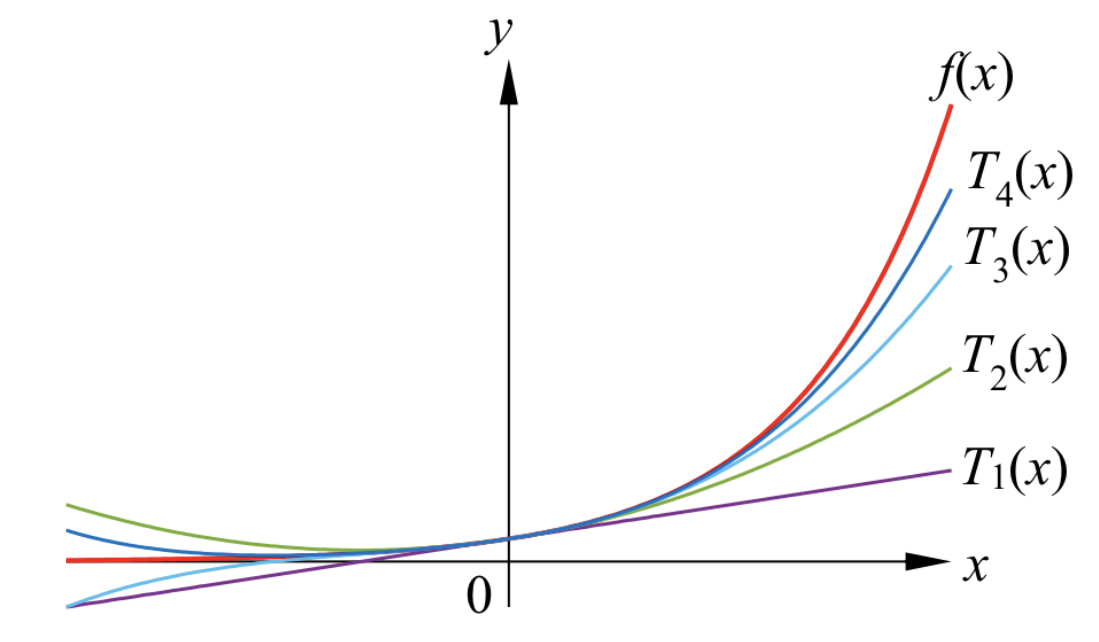
\includegraphics[scale=0.2]{Picture59.png}
\caption{The function $f(x)=e^x$ and its Taylor polynomials at $x=0$.\fa}\label{figure59}
\end{figure}

In Theorem \ref{230307_8}, we apply  mean value theorem to prove that $|\sin x|\leq |x|$ for all real numbers $x$. In the following example, we extend this result partially.
\begin{example}{}
Show that
for $x\in (0, \pi)$,  $\sin x>x-\di\frac{x^3}{6}$.
\end{example}
\begin{solution}{Solution}
Let $f(x)=\sin x$. Then $f(x)$ is infinitely differentiable, with the third  Taylor polynomial at $x=0$ given by
\[ T_3(x)= x-\frac{x^3}{6}.\]
Apply the Lagrange remainder theorem, we find that for any $x\in (0,\pi)$, there is a $\xi \in (0,x)\subset (0,\pi)$ so that
\[\sin x-x+\di\frac{x^3}{6}=\frac{f^{(4)}(\xi)}{24}x^4=\frac{\sin \xi}{24}x^4.\] Since $\sin\xi>0$ for $\xi\in (0,\pi)$,
 this proves that \[\sin x>x-\di\frac{x^3}{6}\hspace{1cm}\text{for}\;x\in (0,\pi).\]
\end{solution}

\begin{figure}[ht]
\centering
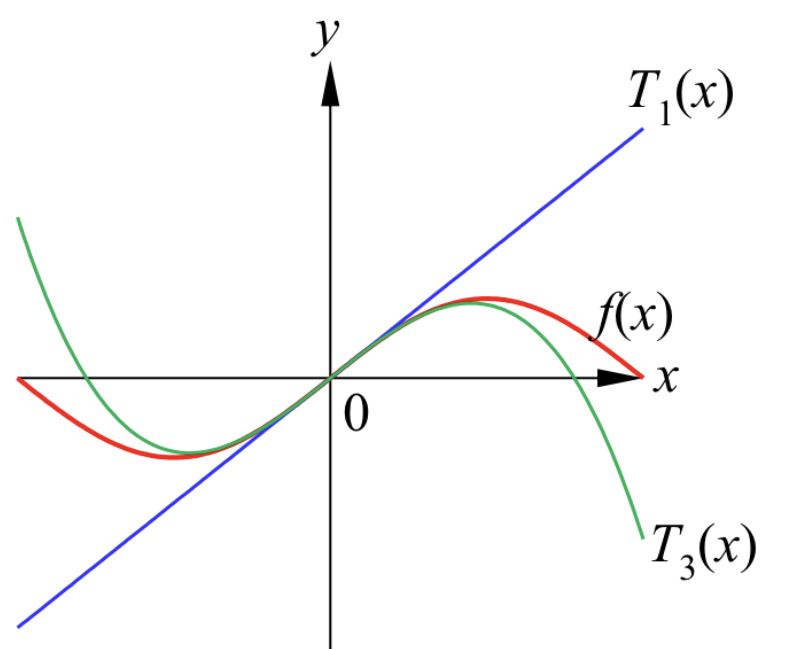
\includegraphics[scale=0.2]{Picture60.png}
\caption{The function $f(x)=\sin x$ and its Taylor polynomials at $x=0$.\fa}\label{figure60}
\end{figure}

  We have repeatedly used the fact that if $f:I\to\mathbb{R}$ is a differentiable function defined on an open interval $I$, and $f'(x)=0$ for all $x\in I$, then $f(x)$ is a constant function. The next theorem extends this result.
\begin{theorem}[label=230307_17]{}
Let $I$ be an open interval, and let $n$ be a positive integer. Assume that the function $f:I\to\mathbb{R}$ is $(n+1)$ times differentiable, and
$f^{(n+1)}(x)=0$ for all $x\in I$. Then $f(x)$ is a polynomial of degree at most $n$.
\end{theorem} 
\begin{myproof}{Proof}If $f^{(n+1)}(x)=0$ for all $x\in I$, take any point $x_0$  in $I$, and let $T_n(x)$ be the $n^{\text{th}}$ Taylor polynomial of $f$ at $x_0$. By definition, $f(x_0)=T_n(x_0)$. Given $x\in I\setminus\{x_0\}$, the Lagrange remainder theorem implies that there is a point $\xi\in I$ such that
\[f(x)-T_n(x)=\frac{f^{(n+1)}(\xi)}{(n+1)!}(x-x_0)^{n+1}.\]
Since $f^{(n+1)}(x)$ is identically 0, we find that for all $x\in I$, 
$f(x)=T_n(x)$. This proves that $f$ is a polynomial of degree at most $n$.

\end{myproof}

As a corollary, we have the following.
\begin{corollary}{}
Let $I$ be an open interval, and let $n$ be a positive integer. Assume that $f:I\to\mathbb{R}$ and $g:I\to\mathbb{R}$ are $(n+1)$ times differentiable functions such that
\[f^{(n+1)}(x)=g^{(n+1)}(x)\hspace{1cm}\text{for all}\;x\in I,\] then there is a polynomial $p(x)$ of degree at most $n$ such that
\[f(x)=g(x)+p(x).\]
\end{corollary}

Next we turn to the Cauchy remainder theorem. In Example \ref{230307_10}, we have shown that if $g:I\to\mathbb{R}$ is a continuous function, $x_0$ is a point in $I$,  $n$ is a positive integer, then  the function $G:I\to\mathbb{R}$ defined by
\[G(x)=\frac{1}{n!}\int_{x_0}^x(x-t)^ng(t)dt \]
  is $(n+1)$ times continuously differentiable,  
\[G(x_0)=G'(x_0)=\ldots=G^{(n)}(x_0)=0,\]
and
\[G^{(n+1)}(x)=g(x)\hspace{1cm}\text{for all}\;x\in I.\]
\begin{theorem}{The Cauchy Remainder Formula}
Let $I$ be an open interval that contains the point $x_0$, and let $n$ be a positive integer. Given that $f:I\to\mathbb{R}$   is a function that is $(n+1)$ times continuously differentiable, let \[T_n(x)=\di\sum_{k=0}^n\frac{f^{(k)}(x_0)}{k!}(x-x_0)^k\]be its Taylor polynomial of order $n$ at $x_0$. For any $x\in I$,  
\[f(x)-T_n(x)=\frac{1}{n!}\int_{x_0}^x (x-t)^n f^{(n+1)}(t)dt.\]

\end{theorem}
\begin{myproof}{Proof}
Let $H: I\to\mathbb{R}$ be the function defined by
\[H(x)=f(x)-T_n(x)-\frac{1}{n!}\int_{x_0}^x (x-t)^n f^{(n+1)}(t)dt.\]
Then by the result proved in Example \ref{230307_10}, we find that $H$ is a function that is $(n+1)$ times continuously differentiable,
\[H(x_0)=H'(x_0)=\cdots=H^{(n)}(x_0)=0,\]
and
\[H^{(n+1)}(x)=f^{(n+1)}(x)-f^{(n+1)}(x)=0\hspace{1cm}\text{for all}\;x\in I.\]
By Theorem \ref{230307_17} and Corollary \ref{230307_18}, $H(x)=0$ for all $x\in I$. This completes the proof of the assertion.
\end{myproof}

In Cauchy remainder formula, the error term is expressed as a precise integral, although in practice it might not be possible to evaluate such an integral. Let us now apply the Cauchy remainder formula to prove that the Maclaurin series of the function $f(x)=(1+x)^{\alpha}$ converges to $f(x)$ when $x\in (-1,1)$.
\begin{theorem}
{}Let $\alpha$ be a real number. For $|x|<1$,
\[(1+x)^{\alpha}= \sum_{k=0}^{\infty}\binom{\alpha}{k}x^k.\]
\end{theorem}
\begin{myproof}{Proof}Let $f(x)=(1+x)^{\alpha}$, $-1<x<1$. We have seen that $\di \sum_{k=0}^{\infty}\binom{\alpha}{k}x^k$ is the Maclaurin series of $f(x)$.
The $n^{\text{th}}$ Taylor polynomial of $f(x)$ at $x=0$ is 
\[T_n(x)=\sum_{k=0}^{n}\binom{\alpha}{k}x^k.\]\bp
We need to show that $\di \lim_{n\to\infty}T_n(x)=f(x)$ for all $|x|<1$.
It is easy to verify that
\[f^{(n+1)}(x)= (n+1)! \binom{\alpha}{n+1}(1+x)^{\alpha-n-1}.\]
By  Cauchy remainder formula,  for $x\in (-1,1)$,
\begin{align*}f(x)-T_n(x)&=\frac{1}{n!}\int_0^x (x-t)^nf^{(n+1)}(t)dt\\&=(n+1)\binom{\alpha}{n+1}\int_0^x(x-t)^n(1+t)^{\alpha-n-1}dt.\end{align*}
We  need to  estimate this last integral for $x\neq 0$. Making a change of variables $t=x\tau$, we find that
\[\int_0^x(x-t)^n(1+t)^{\alpha-n-1}dt=x^{n+1}\int_0^1 (1-\tau)^n(1+x\tau)^{\alpha-n-1}d\tau.\]
Notice that since $x\in (-1,1)$, when $\tau\in [0,1]$, 
\[(1-\tau)^n(1+x\tau)^{\alpha-n-1}\geq 0.\]  For fixed $x\in (-1,1)$, the function $g:[0,1]\to\mathbb{R}$, $g(\tau)=(1+x\tau)^{\alpha-1}$ is continuous.   Therefore, there is a constant $M$ such that 
\[0\leq (1+x\tau)^{\alpha-1}\leq M\hspace{1cm}\text{for all}\;\tau\in [0,1].\]
This implies that
\[0\leq \int_0^1 (1-\tau)^n(1+x\tau)^{\alpha-n-1}d\tau\leq M\int_0^1\left(\frac{1-\tau}{1+x\tau}\right)^{n}d\tau.\]
For any $x\in (-1,1)$ and $\tau\in [0,1]$,
\[1+x\tau\geq 1-\tau\geq 0.\]
 This  implies that for any $x\in (-1,1)$, 
\[0\leq \left(\frac{1-\tau}{1+x\tau}\right)^{n} \leq 1\hspace{1cm}\text{for all}\;\tau\in [0,1].\]\bp
Therefore, we find that
\[0\leq \int_0^1\left(\frac{1-\tau}{1+x\tau}\right)^{n}d\tau\leq 1\hspace{1cm}\text{for all}\;|x|<1.\]Hence,
\begin{equation}\label{eq230307_13}|f(x)-T_n(x)|\leq M (n+1)\left|\binom{\alpha}{n+1}x\right|^{n+1}.\end{equation}
In Example \ref{230307_9}, we have proved that the series $\di\sum_{n=0}^{\infty}\binom{\alpha}{n}x^n$ is convergent when $|x|<1$. It follows from Theorem \ref{230305_15} that the derived series $\di\sum_{n=0}^{\infty}(n+1)\binom{\alpha}{n+1}x^n$ is also convergent when $|x|<1$. This implies that 
\[\lim_{n\to\infty}(n+1)\left|\binom{\alpha}{n+1}x\right|^n=0.\]
Using squeeze theorem, we deduce from \eqref{eq230307_13} that
\[\lim_{n\to\infty}T_n(x)=f(x).\] This completes the proof.
\end{myproof}


\vp
\noindent
{\bf \large Exercises  \thesection}
\setcounter{myquestion}{1}
\begin{question}{\themyquestion}
Let $f:\mathbb{R}\to\mathbb{R}$ be the function defined by
\[f(x)=\begin{cases} \di\frac{2-2\cos x}{x^2},\quad &\text{if}\;x\neq 0,\\1,\quad & \text{if} \;x=0.\end{cases}\]Show that  $f$ is infinitely differentiable, and find $f^{(n)}(0) $ for all $n\geq 0$.
\end{question}


\atc
\begin{question}{\themyquestion}
Show that for all $x>0$,
\[x-\frac{x^2}{2}<\ln (1+x)<x.\]
\end{question}
 
\atc
\begin{question}{\themyquestion}
Show that for all $x>0$,
\[1+\frac{x}{2}-\frac{x^2}{8}<\sqrt{1+x}<1+\frac{x}{2}-\frac{x^2}{8}+\frac{x^3}{16}.\]
\end{question}

\atc
\begin{question}{\themyquestion}
Show that for all $x\in (-\pi, \pi)$,
\[\cos x\geq 1-\frac{x^2}{2}.\]
\end{question}

\atc
\begin{question}{\themyquestion}
Let $\alpha$ be a real number. Assume that $\alpha$ is not an integer. In Example \ref{230307_9}, we have shown that the power series $\di\sum_{k=0}^{\infty}\binom{\alpha}{k}x^k$,
which is the Maclaurin series of the function $f(x)=(1+x)^{\alpha}$, has radius of convergence 1. Define the function 
$g:(-1,1)\to\mathbb{R}$ by
\[g(x)=\sum_{k=0}^{\infty}\binom{\alpha}{k}x^k.\]
In this question, you are asked to show that $g(x)=(1+x)^{\alpha}$ for $x\in (-1,1)$, without using the Cauchy remainder formula.
\begin{enumerate}[(a)]\item
Show that $(1+x)g'(x)=\alpha g(x)$ for all $x\in (-1,1)$.
\item Let $h:(-1,1)\to\mathbb{R}$ be the function defined by $h(x)=g(x)(1+x)^{-\alpha}$. Prove that $h$ is a constant function.
\item Conclude that $g(x)=(1+x)^{\alpha}$ for all $x\in (-1,1)$.
\end{enumerate}
\end{question}

\vp


\section{Examples and Applications}\label{sec6.6}
In this section, we discuss some examples and applications.

The number $e$ and the number $\pi$ are two important numbers in mathematics. 
In Section \ref{sec6.6.1} and Section \ref{sec6.6.2}, we prove respectively that these two numbers are irrational. 

In Section \ref{sec6.6.3}, we prove that there is an infinitely differentiable function whose Taylor series at a point does not converge to the function itself. We also briefly discuss the applications of such functions, despite its non-analyticity.


In Section \ref{sec6.6.4}, we construct a continuous function that is differentiable nowhere. It uses Theorem \ref{230304_1} which says that uniform limit of continuous functions is continuous.

 
In Section \ref{sec6.6.5}, we prove the Weierstrass approximation theorem, which says that any continuous function defined on a closed and bounded interval can be uniformly approximated by a polynomial. We give a proof that uses Bernstein's approach. It uses the fact that a continuous function defined on a closed and bounded interval is bounded and uniformly continuous.  Later when we study Fourier series, we are going to prove this important theorem again using the theory of Fourier series.
 

\subsection[The Irrationality of $e$]{The Irrationality of $\pmb{e}$}\label{sec6.6.1}
In Example \ref{23020507}, we have defined the number $e$ as the limit of the increasing sequence $\{a_n\}$, where $\di a_n=\left(1+\frac{1}{n}\right)^n$. We have proved that $a_n\leq 3$ for all $n\in\mathbb{Z}^+$. This implies that $e\leq 3$. In Theorem \ref{230307_6}, we proved that
\[e=\sum_{n=0}^{\infty}\frac{1}{n!}=1+\frac{1}{1!}+\frac{1}{2!}+\cdots+\frac{1}{n!}+\cdots.\]

\begin{theorem}{Irrationality of $\pmb{e}$}
The number $e$ is irrational.
\end{theorem}
\begin{myproof}{Proof}Assume to the contrary that $e$ is rational. Then since $e$ is positive, there are positive integers $a$ and $b$ such that
\[e=\frac{a}{b}.\]
For any positive integer $n$, we apply  Lagrange remainder theorem to the $n^{\text{th}}$ Taylor polynomial of $e^x$ at the point $x_0=0$. With $x=1$, we find that there is a number $c_n$ in the interval $(0,1)$ such that
\begin{equation}\label{eq230307_20}e=1+\frac{1}{1!}+\frac{1}{2!}+\cdots+\frac{1}{n!}+\frac{e^{c_n}}{(n+1)!}.\end{equation} 
 
For $n\geq b$, we find that
$n!$ is divisible by $b$, and so $n!e$ is an integer. From \eqref{eq230307_20}, we have
\[0<n!e-\left(n!+n!+\frac{n!}{2!}+\cdots+\frac{n!}{n!}\right)=\frac{e^{c_n}}{n+1}<\frac{e}{n+1}\leq  \frac{3}{n+1}.\]
Notice that for each $1\leq k\leq n$, $n!/k!$ is an integer. Hence, for $n\geq b$, 
\[n!e-\left(n!+n!+\frac{n!}{2!}+\cdots+\frac{n!}{n!}\right)\] is a positive integer that is less than $3/(n+1)$. For $n>3$, $3/n+1$ is less than 1. This gives a contradiction. Hence, $e$ must be irrational.
\end{myproof}

\bigskip
\subsection[The Irrationality of $\pi$]{The Irrationality of $\pmb{\pi}$}\label{sec6.6.2}

As in the case of the number $e$, we will show that $\pi$ is an irrational number using proof by contradiction. 
We begin by two lemmas.
\begin{lemma}[label=230309_1]{}
Given that $f:\mathbb{R}\to\mathbb{R}$ and $g:\mathbb{R}\to\mathbb{R}$ are two infinitely differentiable functions. For any $n\in\mathbb{Z}^+$, and any numbers $\alpha$ and $\beta$,
\begin{equation}\label{eq230308_1}\begin{split}
&\int_{\alpha}^{\beta} f^{(2n+1)}(x)g(x)dx+\int_{\alpha}^{\beta} f(x)g^{(2n+1)}(x)dx\\ &=\sum_{k=0}^{2n}(-1)^k f^{(k)}(\beta)g^{(2n-k)}(\beta)-\sum_{k=0}^{2n}(-1)^k f^{(k)}(\alpha)g^{(2n-k)}(\alpha).
\end{split}\end{equation}

\end{lemma}
\begin{myproof}{Proof}Given  $n\in\mathbb{Z}^+$,
define the function $F:\mathbb{R}\to\mathbb{R}$ by
\[F (x)=\sum_{k=0}^{2n}(-1)^k f^{(k)}(x)g^{(2n-k)}(x).\]
Then
\[
F'(x) =\sum_{k=0}^{2n}(-1)^kf^{(k+1)}(x)g^{(2n-k)}(x)+\sum_{k=0}^{2n}(-1)^kf^{(k)}(x)g^{(2n-k+1)}(x)\]Because of the alternating signs, the $k=0$ to $k=2n-1$ terms in the first sum cancel with the $k=1$ to $k=2n$ terms in the second sum.  This gives
\[
F'(x)=f^{(2n+1)}(x)g(x)+f(x)g^{(2n+1)}(x).
\]  By fundamental theorem of calculus, we find that  
\[
F(\beta)-F(\alpha)=\int_{\alpha}^{\beta} f^{(2n+1)}(x)g(x)dx+\int_{\alpha}^{\beta} f(x)g^{(2n+1)}(x)dx.
\]This proves \eqref{eq230308_1}.
\end{myproof}

\begin{lemma}[label=230309_2]{}
Let $a$, $b$ and $n$ be positive integers. Define the polynomial $p:\mathbb{R}\to\mathbb{R}$ by
\[p(x)=\frac{x^n(a-bx)^n}{n!}.\]
For any  integer $k$ satisfying $0\leq k\leq 2n$, $p^{(k)}(0)$ and $p^{(k)}(a/b)$ are integers.
\end{lemma}
\begin{myproof}{Proof} 
Using binomial expansion, we have
\[p(x)=\frac{x^n}{n!}\sum_{m=0}^n \binom{n}{m}a^{n-m}(-1)^mb^mx^m.\]
By Lemma \ref{230307_4},
\[p(x)=\sum_{k=0}^{2n}\frac{p^{(k)}(0)}{k!}x^k.\] 
Comparing the coeficients, we find that   
\begin{align*}
p^{(k)}(0)=\begin{cases}0,\quad &\text{if}\; \;0\leq k\leq n-1,\\ \di
 \frac{k!}{n!}\binom{n}{k-n}a^{2n-k}(-1)^{k-n}b^{k-n},\quad &\text{if}\;\;n\leq k\leq 2n.\end{cases}\end{align*}Since $k!$ is divisible by $n!$ when $k\geq n$, we find  that $p^{(k)}(0)$ is an integer for all $0\leq k\leq 2n$.
Expanding $p(x)$ in powers of $(x-a/b)$, we find that
\begin{align*}
p(x)=(-1)^n\frac{b^n}{n!}\left(x-\frac{a}{b}\right)^n\sum_{m=0}^n\binom{n}{m}\left(\frac{a}{b}\right)^{n-m}\left(x-\frac{a}{b}\right)^m.
\end{align*}
By Lemma \ref{230307_4},
\[p(x)=\sum_{k=0}^{2n}\frac{p^{(k)}(a/b)}{k!}\left(x-\frac{a}{b}\right)^k.\]  \bp
Comparing the coeficients, 
we find that
\begin{align*}p^{(k)}\left(\frac{a}{b}\right)=\begin{cases}0,\quad &\text{if}\; \;0\leq k\leq n-1,\\ \di (-1)^n\frac{k!}{n!}\binom{n}{k-n}a^{2n-k}b^{k-n},\quad &\text{if}\;\;n\leq k\leq 2n.\end{cases}\end{align*}
Hence, $p^{(k)}(a/b)$ is also an integer  for all $0\leq k\leq 2n$.
\end{myproof}

Now we can prove the theorem.
\begin{theorem}{Irrationality of $\pmb{\pi}$}
The number $\pi$ is irrational.

\end{theorem}
\begin{myproof}{Proof}


Assume that $\pi$ is a rational number. Then there are positive integers $a$ and $b$ such that \[\pi =\frac{a}{b}.\] For   $n\in\mathbb{Z}^+$, define the polynomial $p_{n}(x)$ by
\[p_n(x)=\frac{x^n(a-bx)^n}{n!}=\frac{b^nx^n(\pi-x)^n}{n!},\]and let
\[I_n=\int_0^{\pi}p_n(x)\sin xdx.\]
Take $f(x)=p_n(x)$, $g(x)=\cos x$ and $\alpha=0$, $\beta=\pi$ in Lemma \ref{230309_1}. 
Since $p_n(x)$ is a polynomial of degree $2n$, we find that $p_n^{(2n+1)}(x)=0$. On the other hand, for all $k\geq 0$,
\begin{gather*}
g^{(4k)}(x)=\cos x, \quad g^{(4k+1)}(x)=-\sin x,\\g^{(4k+2)}(x)=-\cos x,\quad g^{(4k+3)}(x)=\sin x.\end{gather*}\bp
In particular,  $g^{(2n+1)}(x)=(-1)^{n-1}\sin x$. 
 From \eqref{eq230308_1}, we have
\begin{equation}\label{eq230309_3}\begin{split}
I_n &= (-1)^{n-1}\left\{\sum_{k=0}^{2n}(-1)^k p_n^{(k)}(\pi)g^{(2n-k)}(\pi)\right.\\&\hspace{3cm}\left.-\sum_{k=0}^{2n}(-1)^k p_n^{(k)}(0)g^{(2n-k)}(0)\right\}.\end{split}
\end{equation}By Lemma \ref{230309_2}, $p_n^{(k)}(0)$ and $p_n^{(k)}(\pi)$ are  integers for all $0\leq k\leq 2n$. Since
\[\sin 0=0,\quad \sin \pi =0, \quad \cos 0=1,\quad \cos \pi =-1\] are   integers, we find that $g^{(k)}(0)$ and $g^{(k)}(\pi)$ are  integers for all $k\geq 0$. The right hand side of \eqref{eq230309_3} shows  that $I_n$ is an integer for all $n\in\mathbb{Z}^+$. 
On the other hand, for all $0\leq x\leq \pi$,
\[0\leq x(\pi -x)\leq \left(\frac{\pi}{2}\right)^2.\]
Therefore, for $0\leq x\leq \pi$, 
\[0\leq p_n(x)\leq \frac{1}{n!}\left(\frac{\pi^2 b}{4}\right)^n.\]
Since we also have $0\leq\sin x\leq 1$ for all $0\leq x\leq \pi$, we conclude that
\[0\leq I_n=\int_0^{\pi}p_n(x)\sin x dx\leq  \frac{\pi}{n!}\left(\frac{\pi^2 b}{4}\right)^n.\] 
Because the series $\di\sum_{n=0}^{\infty} \frac{1}{n!}\left(\frac{\pi^2 b}{4}\right)^n$ is convergent, we find that 
\[\lim_{n\to\infty}  \frac{1}{n!}\left(\frac{\pi^2 b}{4}\right)^n=0.\]Therefore, there is a positive integer $N$ such that for all $n\geq N$,
\[  \frac{1}{n!}\left(\frac{\pi^2 b}{4}\right)^n<\frac{1}{\pi},\]
which gives
\[0\leq I_n<1\hspace{1cm}\text{for all}\;n\geq N.\]\bp
We only need the $n=N$ case now. Since $I_N$ is an integer, we must have $I_N=0$. However, since 
\[p_{N}(x)\sin  x\] is a  continuous function and it is positive on $(0,\pi)$, by Example \ref{ex230222_5}, \[I_N=\di\int_0^{\pi}p_N(x)\sin xdx\] cannot be zero. This gives a contradiction. Hence, $\pi$ must be an irrational number. 

\end{myproof}

\bigskip
\subsection{ Infinitely Differentiable Functions that are Non-Analytic}\label{sec6.6.3}
We consider the function $f:\mathbb{R}\to\mathbb{R}$ defined by
\begin{equation*} f(x)=\begin{cases}\di\exp\left(-\frac{1}{x^2}\right),\quad &\text{if}\;x\neq 0,\\0,\quad &\text{if}\;x=0.\end{cases}\end{equation*}
We will show that this function  is infinitely differentiable and $f^{(n)}(0)=0$ for all $n\geq 0$. 
 
\begin{figure}[ht]
\centering
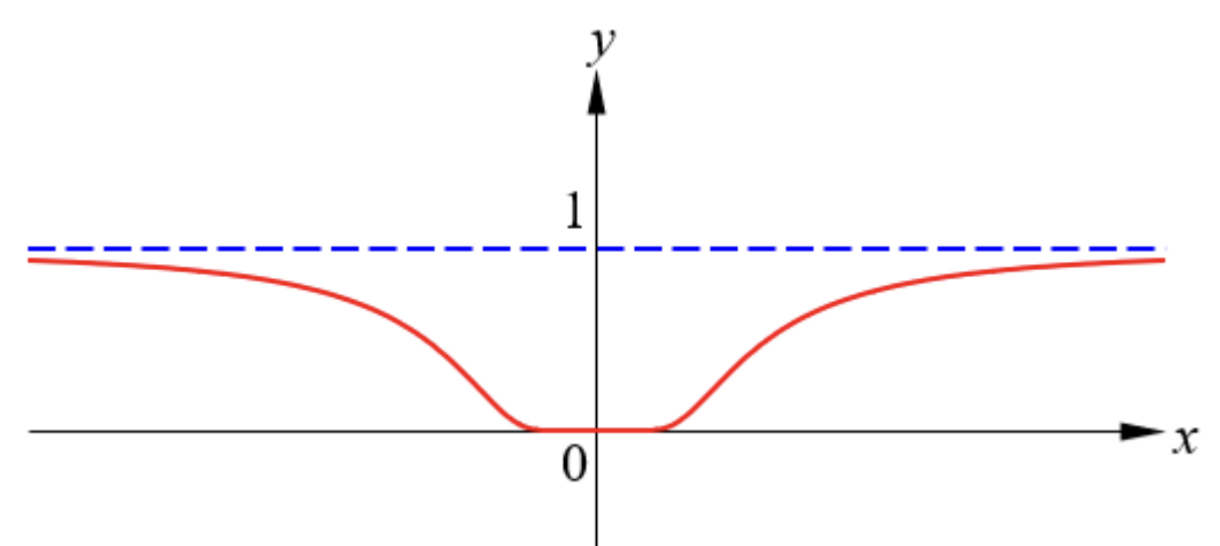
\includegraphics[scale=0.2]{Picture58.png}
\caption{The function $\di f(x)=\exp\left(-\frac{1}{x^2}\right)$.\fa}\label{figure58}
\end{figure}


Let us first prove the following lemma.
\begin{lemma}[label=230309_6]{}
If $p(x)$ is a polynomial, then
\begin{subequations}\label{eq230309_4}\begin{align}\lim_{x\to 0^+}p\left(\frac{1}{x}\right)\exp\left(-\frac{1}{x}\right)=0 \label{eq230309_4_1}\\
\lim_{x\to 0}p\left(\frac{1}{x}\right)\exp\left(-\frac{1}{x^2}\right)=0.\label{eq230309_4_2}
\end{align}\end{subequations}
\end{lemma}\begin{myproof}{Proof}
In Example \ref{230307_11}, we have shown that for any  real number $s$,
$\di \lim_{y\to \infty}y^s e^{-y}=0$. From this, we find that
 if $k$ is an integer,
\[\lim_{x\to 0^+}\frac{1}{x^k}\exp\left(-\frac{1}{x}\right)=\lim_{y\to \infty}y^ke^{-y}=0,\] and 
\[\lim_{x\to 0}\frac{1}{x^{2k}}\exp\left(-\frac{1}{x^2}\right)=\lim_{y\to \infty}y^ke^{-y}=0.\]
The latter one implies that for any integer $k$,
\[\lim_{x\to 0}\frac{1}{x^{2k-1}}\exp\left(-\frac{1}{x^2}\right)=\left[\lim_{x\to 0}x\right]\left[\lim_{x\to 0}\frac{1}{x^{2k}}\exp\left(-\frac{1}{x^2}\right)\right]=0.\]
These prove \eqref{eq230309_4}.
\end{myproof}

Next, we prove the following.
\begin{theorem}[label=230309_7]{}
Let  $f:\mathbb{R}\to\mathbb{R}$ be the function defined by
\begin{equation}\label{eq230307_12}f(x)=\begin{cases}\di\exp\left(-\frac{1}{x^2}\right),\quad &\text{if}\;x\neq 0,\\0,\quad &\text{if}\;x=0.\end{cases}\end{equation}
Then $f$ is an infinitely differentiable function with $f^{(n)}(0)=0$ for all $n\geq 0$.
\end{theorem}

\begin{myproof}{Proof} We claim that for each positive integer $n$, there is a polynomial $p_n(x)$ of degree $3n$ such that
 \begin{equation}
\label{eq230309_5}f^{(n)}(x)=\begin{cases}\di p_n\left(\frac{1}{x}\right)\exp\left(-\frac{1}{x^2}\right),\quad &\text{if}\;x\neq 0,\\0,\quad &\text{if}\;x=0.\end{cases}\end{equation}
This will show that $f$ is infinitely differentiable. In fact, Lemma \ref{230309_6} implies that 
\[\lim_{x\to 0}f_n(x)=\lim_{n\to 0}p_n\left(\frac{1}{x}\right)\exp\left(-\frac{1}{x^2}\right)=0=f^{(n)}(0),\]which says that $f^{(n)}(x)$ is continuous at $x=0$.
We will prove  \eqref{eq230309_5}  by induction on $n$.
When $n=1$, we find from the definition \eqref{eq230307_12} that
\[f'(x)=\frac{2}{x^3}\exp\left(-\frac{1}{x^2}\right)\hspace{1cm}\text{when}\;x\neq 0.\] 

When $x=0$, we apply Lemma \ref{230309_6} to get
\[f'(0)=\lim_{x\to 0}\frac{\di \exp\left(-\frac{1}{x^2}\right)-0}{x}=\lim_{x\to 0}\frac{1}{x}\exp\left(-\frac{1}{x^2}\right)=0.\]Therefore, the $n=1$ statement is true with $p_1(x)$ is polynomial of degree 3 given by
\[p_1(x)=2x^3.\]
Assume that the statement is true for the $n-1$ case. This means that there is a polynomial $p_{n-1}(x)$ of degree   $3n -3$ such that
\[f^{(n-1)}(x)=\begin{cases}\di  p_{n-1}\left(\frac{1}{x }\right)\exp\left(-\frac{1}{x^2}\right),\quad &\text{if}\;x\neq 0,\\0,\quad &\text{if}\;x=0.\end{cases}\]When $x\neq 0$,
\[f^{(n)}(x)=\left( -\frac{1}{x^2}p_{n-1}'\left(\frac{1}{x}\right)+\frac{2}{x^3}p_{n-1}\left(\frac{1}{x}\right)\right)\exp\left(-\frac{1}{x^2}\right).\]\bp This shows that when $x\neq 0$,
\[  f^{(n)}(x)=p_{n}\left(\frac{1}{x }\right)\exp\left(-\frac{1}{x^2}\right),\]
where
\[p_n(x)=-x^2 p_{n-1}'(x)+2x^3p_{n-1}(x).\]
By inductive hypothesis, $p_{n-1}'(x)$ is a polynomial of degree $3n-4$. Thus, $x^2 p_{n-1}'(x)$ is a polynomial of degree $3n-2$. Since $2x^3p_{n-1}(x)$ is a polynomial of degree $3n$, $p_n(x)$ is a polynomial of degree $3n$. 
For the derivative at 0, Lemma \ref{230309_6} implies that
\[f^{(n)}(0)=\lim_{x\to 0}\frac{f^{(n-1)}(x)-f^{(n-1)}(0)}{x}=\lim_{x\to 0}\frac{1}{x}p_{n-1}\left(\frac{1}{x}\right)\exp\left(-\frac{1}{x^2}\right)=0.\]
This proves the statement for the $n$ case, and thus completes the induction.\end{myproof}

Now we prove our main theorem in this section.
\begin{theorem}{}Let $I$ be an open interval that contains the point $x_0$. There is an infinitely differentiable function $f:I\to\mathbb{R}$ whose Taylor series at the point $x=x_0$  is convergent pointwise on $I$, but it does not converge to $f(x)$ pointwise on $I$.
\end{theorem}
\begin{myproof}{Proof}Define the function $f:I\to\mathbb{R}$ by
\begin{equation*} \begin{cases}\di\exp\left(-\frac{1}{(x-x_0)^2}\right),\quad &\text{if}\;x\neq x_0,\\0,\quad &\text{if}\;x=x_0.\end{cases}\end{equation*}Theorem \ref{230309_7} implies  that
 the function $f(x)$  is infinitely differentiable on $I$, and 
$f^{(n)}(x_0)=0$ for all $n\geq 0$. Hence, the Taylor series of $f$ at $x=x_0$,\bp
\[\sum_{n=0}^{\infty}\frac{f^{(n)}(x_0)}{n!}(x-x_0)^n,\] is the series that is identically 0. Therefore, it converges everywhere, but it does not converge to $f(x)$ except at the point $x=x_0$.  
\end{myproof}

 Using almost the same proof as for Theorem \ref{230309_7}, we obtain the following.
\begin{theorem}[label=230309_11]{}
Given a real number $x_0$, the function $g:\mathbb{R}\to\mathbb{R}$ defined by
\begin{equation}\label{eq230309_8}g(x)=\begin{cases} \di\exp\left(-\frac{1}{x-x_0}\right),\quad &\text{if}\;x> x_0,\\0,\quad &\text{if}\;x\leq x_0.\end{cases}\end{equation} is infinitely differentiable.
\end{theorem}



The function $g(x)$ defined by \eqref{eq230309_8} is also not analytic. Nevertheless, it has some important applications. It is usually used to "smooth" up a function or truncate a function smoothly.



\begin{theorem}{}
Given two real numbers $a$ and $b$ with $a<b$, define the function $h:\mathbb{R}\to\mathbb{R}$   by
\begin{equation}\label{eq230309_12}\begin{split}
h(x)&=\frac{g(x-a)}{g(x-a)+g(b-x)}\\&=\begin{cases}
0,\quad &\text{if}\; \quad x\leq a,\\ \di \frac{\di\exp\left(-\frac{1}{x-a}\right)}{\di\exp\left(-\frac{1}{x-a}\right)+\exp\left(-\frac{1}{b-x}\right)},\quad &\text{if}\;a<x<b,\\1,\quad &\text{if}\; \quad x\geq b.\end{cases}\end{split}\end{equation}Then $h$ is a functon that is infinitely differentiable.
\end{theorem}
 
\begin{myproof}{Proof}
We just need to show that $g(x-a)+g(b-x)$ is nonzero for all $x\in\mathbb{R}$. The rest follows from Theorem \ref{230309_11} and the definition of $h(x)$. Since the function $g$ is nonnegative, in order for $g(x-a)+g(b-x)=0$, we must have $g(x-a)=g(b-x)=0$. But we know that $g(x-a)=0$ only  when $x\leq a$, and $g(b-x)=0$ only when $x\geq b$. Since the set $\{x\,|\,x\leq a\}$ and the set $\{x\,|\,x\geq b\}$ are disjoint, we conclude that $g(x-a)+g(b-x)$ is never 0.
\end{myproof}
 
\begin{figure}[ht]
\centering
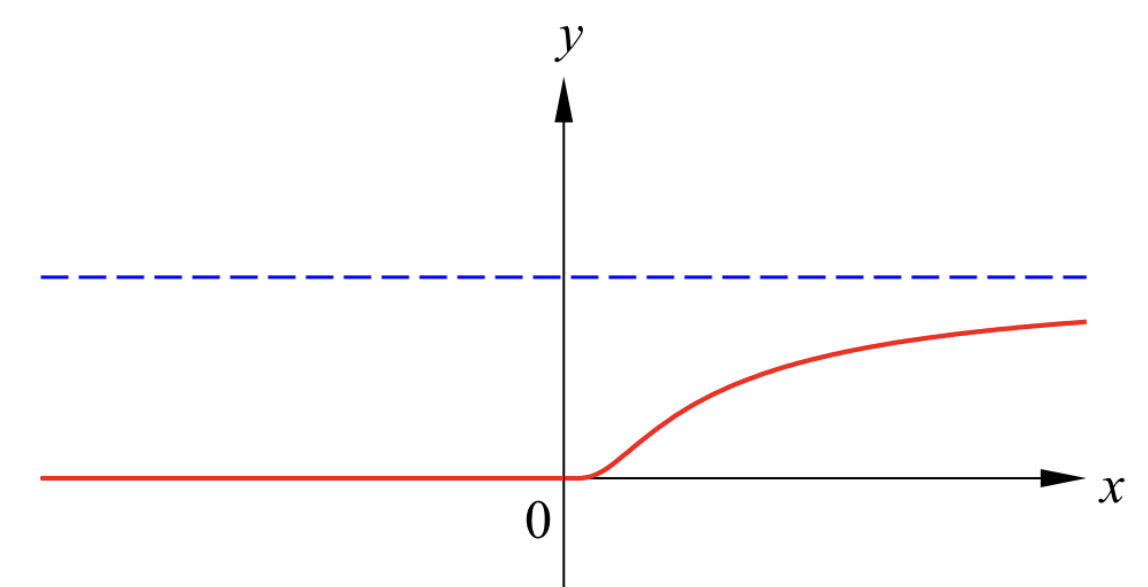
\includegraphics[scale=0.2]{Picture61.png}
\caption{The function $\di g(x)$ defined by \eqref{eq230309_8} when $x_0=0$.\fa}\label{figure61}
\end{figure}

\begin{figure}[ht]
\centering
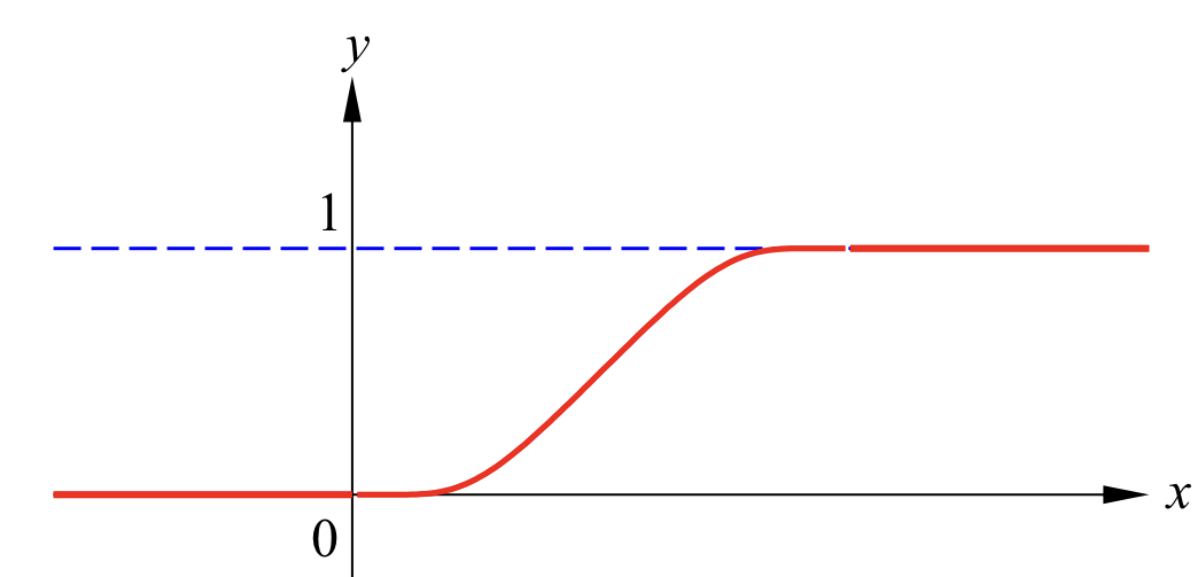
\includegraphics[scale=0.2]{Picture62.png}
\caption{The function $\di h(x)$ defined by \eqref{eq230309_12}.\fa}\label{figure62}
\end{figure}

\begin{remark}{}
The function $h(x)$ defined  by \eqref{eq230309_12}  is an example of an infinitely diferentiable function that is increasing but assume constant values outside a bounded interval.
\end{remark}



\bigskip
\subsection{A Continuous Function that is Nowhere Differentiable}\label{sec6.6.4}
In this section, we want to construct a continuous function $f:\mathbb{R}\to\mathbb{R}$ which is not differentiable at any point. The main ingredient in the proof is to note that the function $g:\mathbb{R}\to\mathbb{R}$, $g(x)=|x|$ is continuous, and it is not differentiable at $x=0$. 

\begin{definition}[label=230309_10]{The function $\pmb{h_m}$}
For any positive number $m$, let $h_m:\mathbb{R}\to\mathbb{R}$ be the function defined by
\[h_m(x)=|x|,\hspace{1cm}\text{for all}\;-m\leq x\leq m,\]
and
\[h_m(x+2m)=h(x)\hspace{1cm}\text{for all}\;x\in\mathbb{R}.\]

\end{definition}

\begin{figure}[ht]
\centering
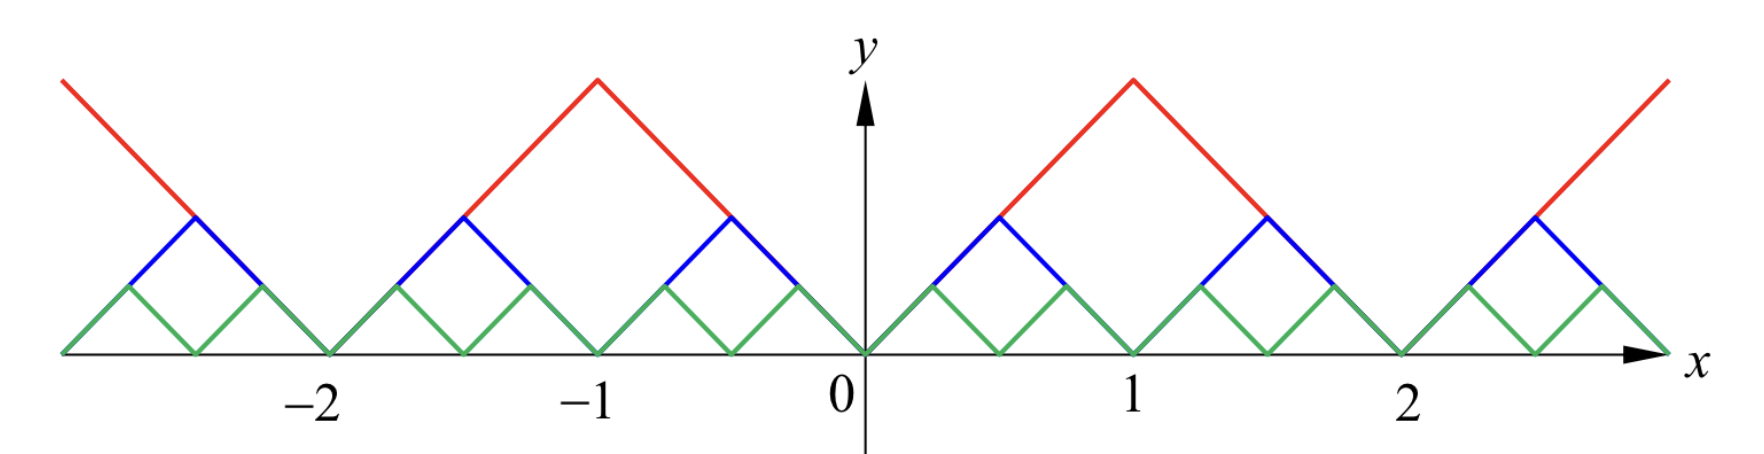
\includegraphics[scale=0.2]{Picture63.png}
\caption{The functions $\di h_m(x)$ when $m=1$, $\frac{1}{2}$ and $\frac{1}{4}$.\fa}\label{figure63}
\end{figure}

 Let us first explore the properties of the function $h_m$.
\begin{lemma}[label=230309_9]{}
Given  a positive number $m$, define $x_{m,k}=mk$ for all $k\in\mathbb{Z}^+$. The function $h_m$ defined in Definition \ref{230309_10} has the following properties.
\begin{enumerate}[(a)]
\item $h_m$  is a continuous even function that is periodic of period $2m$.
\item For $k\in \mathbb{Z}$,  the graph of $h_m:[x_{m,2k}, x_{m, 2k+1}]\to\mathbb{R}$ is a straightline segment of slope 1; while the graph of $h_m:[x_{m,2k-1}, x_{m, 2k}]\to\mathbb{R}$ is a straightline segment of slope $-1$. Hence, the graph  of $h_m$ is a union of straightline segments alternatingly having slopes 1 and $-1$.
\item $0\leq h_m(x)\leq m$ for all $x\in\mathbb{R}$.
\end{enumerate}
\end{lemma}
\begin{myproof}
{Proof}
Part (a) follows from $h_m(-m)=h_m(m)$. Part (b) can be proved by  induction on $k\geq 0$, using the periodicity of $h_m$ and the fact that $h_m$ is an even function.  Part (c) follows from the definition of $h_m$ and periodicity.
\end{myproof}

\begin{lemma}[label=230309_13]{}
Given  a positive number $\ell$ and a point  $x\in \mathbb{R}$, let \[U=[x-\ell /2, x]\hspace{1cm} \text{and} \hspace{1cm} V=[x,x+\ell/2].\] For a positive integer $m$, let $h_m:\mathbb{R}\to\mathbb{R}$ be the function defined in Definition \ref{230309_10}. Then  one of the following holds.
 
\begin{enumerate}[(a)]
\item For each nonnegative integer $k$, the graph of $h_{2^k\ell}:U\to\mathbb{R}$ is a line segment of slope 1 or $-1$.

\item  For each nonnegative integer $k$, the graph of $h_{2^k\ell}:V\to\mathbb{R}$ is a line segment of slope 1 or $-1$.

\end{enumerate}
\end{lemma}
\begin{myproof}{Proof} 
The points $n\ell$, $n\in\mathbb{Z}$, partition the real line into subintervals of the form $[n\ell, (n+1)\ell]$, each of length $\ell$. Since $U$ and $V$ are adjacent intervals of length $\ell/2$, one of them must lie entirely inside one of the intervals of the form $[n\ell, (n+1)\ell]$.
 



 By part (b) in Lemma \ref{230309_9}, the graph of $h_{\ell}:[n\ell, (n+1)\ell]\to\mathbb{R}$ is a line segment of slope 1 or $-1$. This proves the assertion when $k=0$. To prove the assertion for $k\geq 1$, we notice that to obtain the graph of the function $h_{\ell}$ from the graph of the function $h_{2\ell}$, we divide each line segment in the graph of $h_{2\ell}$ into two equal parts, one of the parts change slope from 1 to $-1$ or from $-1$ to $1$. Hence, if $W$ is an interval and the graph of $h_{\ell}:W\to\mathbb{R}$ is a line segment, the graph of $h_{2^k\ell}:W\to\mathbb{R}$ must also be a line segment for any $k\in\mathbb{Z}^+$. This completes the proof the the lemma.
\end{myproof}

Now we can prove the main theorem in this section.

\begin{theorem}
{}For a positive number $m$, let $h_m:\mathbb{R}\to\mathbb{R}$ be the function
\[h_m(x)=|x|\;\;\text{for }\;|x|\leq m, \quad \text{and}\quad h(x+2m)=h(x)\;\;\text{for all}\;x\in\mathbb{R}.\]For $n\geq 0$, let $g_n:\mathbb{R}\to\mathbb{R}$ be the function defined by
$g_n(x)=h_{m_n}(x)$, with $m_n=\di\frac{1}{4^n}$. 
Then the series $\di \sum_{n=0}^{\infty}g_n(x)$ converges uniformly to a function  $f:\mathbb{R}\to\mathbb{R}$,  \[ f(x)=\sum_{n=0}^{\infty}g_n(x).\] $f(x)$ is  a continuous function that is not differentiable at any point.
\end{theorem}
\begin{myproof}{Proof}
 By Lemma \ref{230309_9}, for each $n\in\mathbb{Z}^+$, the function $g_n:\mathbb{R}\to\mathbb{R}$ is continuous and 
\[|g_n(x)|\leq\frac{1}{4^n}\hspace{1cm}\text{for all}\;x\in\mathbb{R}.\]   Since the series $\di\sum_{n=0}^{\infty}\frac{1}{4^n}$ is convergent,
  Weierstrass $M$-test implies that the series $\di \sum_{n=0}^{\infty}g_n(x)$ converges uniformly on $\mathbb{R}$.  Since each $g_n(x)$ is a continuous function,   Corollary \ref{230305_10} implies that  the function  
$\di f(x)=\sum_{n=0}^{\infty}g_n(x)$ is continuous.


 Now we are left to prove that $f(x)$ is not diferentiable at any $x\in \mathbb{R}$. Given $x_0\in \mathbb{R}$, assume that 
\[f'(x_0)=\lim_{x\to x_0}\frac{f(x)-f(x_0)}{x-x_0}\] exists. Then for any sequence $\{x_k\}_{k=0}^{\infty}$ in $\mathbb{R}\setminus\{x_0\}$,  if $\di \lim_{k\to\infty}x_k=x_0$, then the limit  
\[\lim_{k\to \infty}\frac{f(x_k)-f(x_0)}{x-x_0}\]exists and is equal to $f'(x_0)$.\bp

We construt a sequence $\{x_{k}\}_{k=0}^{\infty}$ as follows.  For each $k\in \mathbb{Z}^+$, Lemma \ref{230309_13} implies that either the graph of $
h_{m_k}:[x_0-m_k/2, x_0]\to\mathbb{R}$ or the graph of $h:[x_0, x_0+m_k/2]\to\mathbb{R}$ is a line segment with slope 1 or $-1$.   In the former case, we let $x_{k}=x_0-m_k/2$. In the latter case, we let $x_{k}=x_0+m_k/2$. In any case, we find that
\[|x_{k}-x_0|=\frac{m_k}{2}=\frac{1}{2^{2k+1}}\hspace{1cm}\text{for all}\;k\geq 0.\]
This shows that $\{x_{k}\}$ is a sequence in $\mathbb{R}\setminus\{x_0\}$ that converges to $x_0$. 

For fixed $k\in \mathbb{Z}^+$, 
$m_k/2$ is a multiple of $2m_n$ for all $n>k+1$. By periodicity of $h_{m_n}$, 
\[g_n(x_{k})-g_n(x_0)=h_{m_n}\left(x_0\pm \frac{m_k}{2}\right)-h_{m_n}(x_0)=0\hspace{1cm} \text{for all}\;n>k.\]
This implies that
\[ \frac{f(x_k)-f(x_0)}{x_k-x_0}=\sum_{n=0}^{\infty}\frac{g_n(x_k)-g_n(x_0)}{x_k-x_0}=\sum_{n=0}^{k}\frac{g_n(x_k)-g_n(x_0)}{x_k-x_0}.\]
By the  definition of $x_k$ and Lemma \ref{230309_13}, 
\[\frac{g_n(x_k)-g_n(x_0)}{x_k-x_0}\] is equal to 1 or $-1$ for each $0\leq k\leq n$. The sum of an odd number of 1 or $-1$ must be odd. The sum of an even number of 1 or $-1$ must be even.
Therefore,
\[c_k=\frac{f(x_k)-f(x_0)}{x_k-x_0}\] is odd when $k$ is even, and is even when $k$ is odd. 
This implies that the sequence $\{c_k\}_{k=0}^{\infty}$ is an integer sequence that is alternatingly odd and even. Hence, it does not have a limit. This is a contradiction, which allows us to  conclude that $f$ cannot be differentiable at $x_0$. 
 

\end{myproof}

\begin{figure}[ht]
\centering
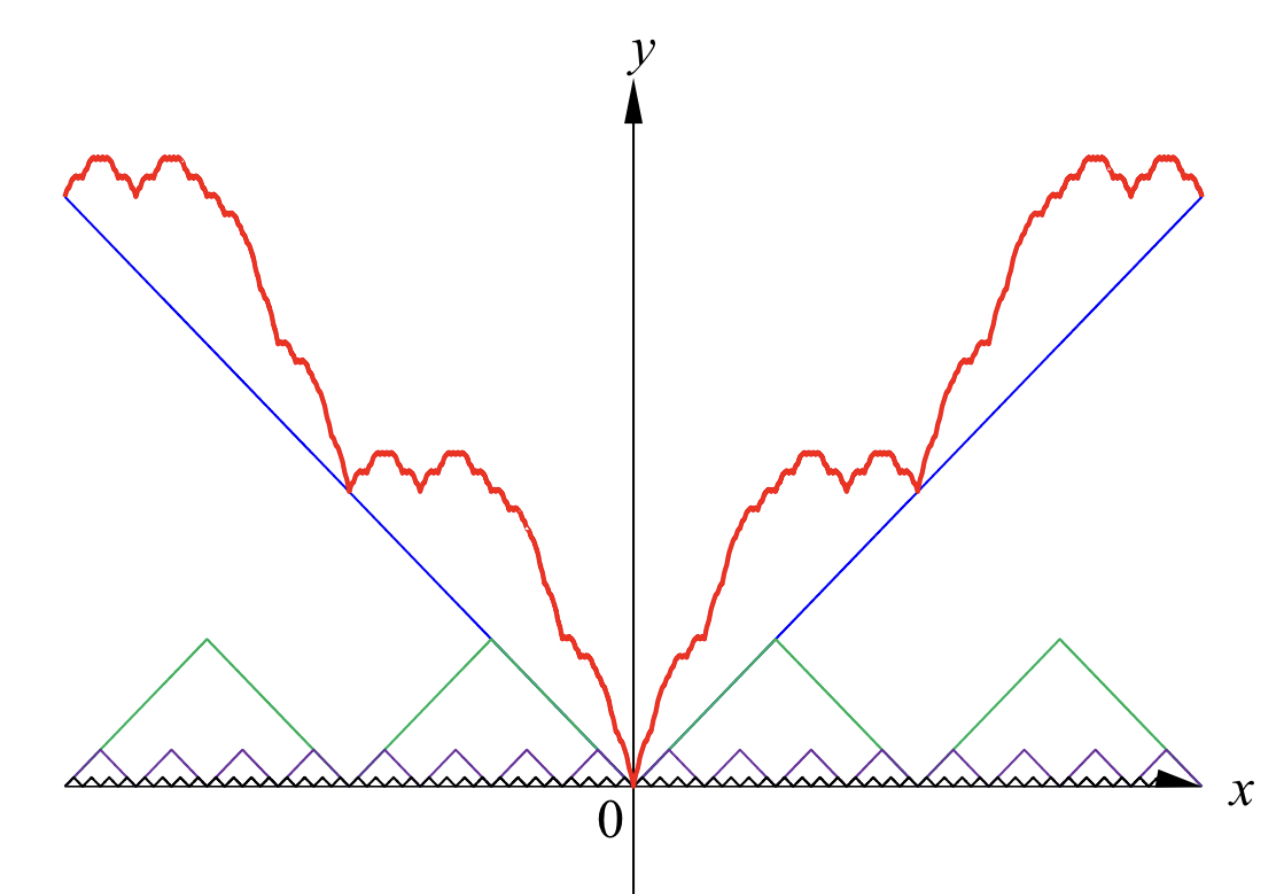
\includegraphics[scale=0.18]{Picture64.png}
\caption{The functions $g_n(x)$ for $n=0, 1, 2, 3$, and the function $f(x)$.\fa}\label{figure64}
\end{figure}
 
 \bigskip
\subsection{The Weierstrass Approximation Theorem}\label{sec6.6.5}
In this section, we prove the Weierstrass approximation theorem using Bernstein's ingenious approach. We start with a  lemma.

\begin{lemma}[label=230309_14]{}
The following identities hold.
\begin{enumerate}[(a)]
\item For $n\geq 0$, $\di\sum_{k=0}^n\binom{n}{k}x^k(1-x)^{n-k}=1$.
\item For $n\geq 1$, $\di\sum_{k=1}^n\frac{k}{n}\binom{n}{k}x^k(1-x)^{n-k}=x$.

%\item For $n\geq 2$, $\di\sum_{k=2}^n\frac{k(k-1)}{n(n-1)}\binom{n}{k}x^k(1-x)^{n-k}=x^2$.
\item For $n\geq 2$, $\di\sum_{k=1}^n\frac{k^2}{n^2}\binom{n}{k}x^k(1-x)^{n-k}=x^2+\frac{x(1-x)}{n}$.
\item For $n\geq 2$, $\di\sum_{k=0}^n\left(x-\frac{k}{n}\right)^2\binom{n}{k}x^k(1-x)^{n-k}=\frac{x(1-x)}{n}$.
 \end{enumerate}
\end{lemma}
\begin{myproof}{Proof}
The first  identity  (a)
is just a consequence of the binomial expansion theorem.
\bp
 For the   identity in (b), notice that when $n\geq k\geq 1$,
\[\frac{k}{n}\binom{n}{k}=\frac{(n-1)!}{(k-1)!(n-k)!}=\binom{n-1}{k-1}.\]
Therefore, 
\begin{align*}\sum_{k=1}^n\frac{k}{n}\binom{n}{k}x^k(1-x)^{n-k}&=x\sum_{k=1}^n\binom{n-1}{k-1}x^{k-1}(1-x)^{n-k}\\&=x\sum_{k=0}^{n-1}\binom{n-1}{k}x^k(1-x)^{n-1-k}=x.\end{align*}
 For part (c), we find that when $n\geq k\geq 2$,
\[\frac{k(k-1)}{n(n-1)}\binom{n}{k}=\frac{(n-2)!}{(k-2)!(n-k)!}=\binom{n-2}{k-2}.\]  It follows that
\begin{align*}\sum_{k=2}^n\frac{k(k-1)}{n(n-1)}\binom{n}{k}x^k(1-x)^{n-k} =x^2\sum_{k=0}^{n-2}\binom{n-2}{k}x^k(1-x)^{n-2-k}=x^2.\end{align*}
Writing  $k^2=k(k-1)+k$, we have
\begin{align*}
&\sum_{k=1}^n\frac{k^2}{n^2}\binom{n}{k}x^k(1-x)^{n-k}\\&=\sum_{k=1}^n\frac{k(k-1)}{n^2}\binom{n}{k}x^k(1-x)^{n-k}+\sum_{k=1}^n\frac{k }{n^2}\binom{n}{k}x^k(1-x)^{n-k}\\
&=\frac{n-1}{n}x^2+\frac{1}{n}x=x^2+\frac{x(1-x)}{n}.
\end{align*} 

For the identity in part (d),
  a straightforward computation  gives
\begin{align*}
&\sum_{k=0}^n\left(x-\frac{k}{n}\right)^2\binom{n}{k}x^k(1-x)^{n-k}\\
&= \sum_{k=0}^n\left(x^2- \frac{2k}{n}x+\frac{k^2}{n^2}\right) \binom{n}{k}x^k(1-x)^{n-k}\\
&=x^2-2x^2+x^2+\frac{x(1-x)}{n} =\frac{x(1-x)}{n}.
\end{align*}
\end{myproof}

\begin{definition}{Bernstein Basis Polynomials}
For any positive integer $n$, there are $n+1$ Bernstein basis polynomials given by
\[p_{n,k}(x)=\binom{n}{k}x^k(1-x)^{n-k},\hspace{1cm}0\leq k\leq n.\]
\end{definition}

 \begin{figure}[ht]
\centering
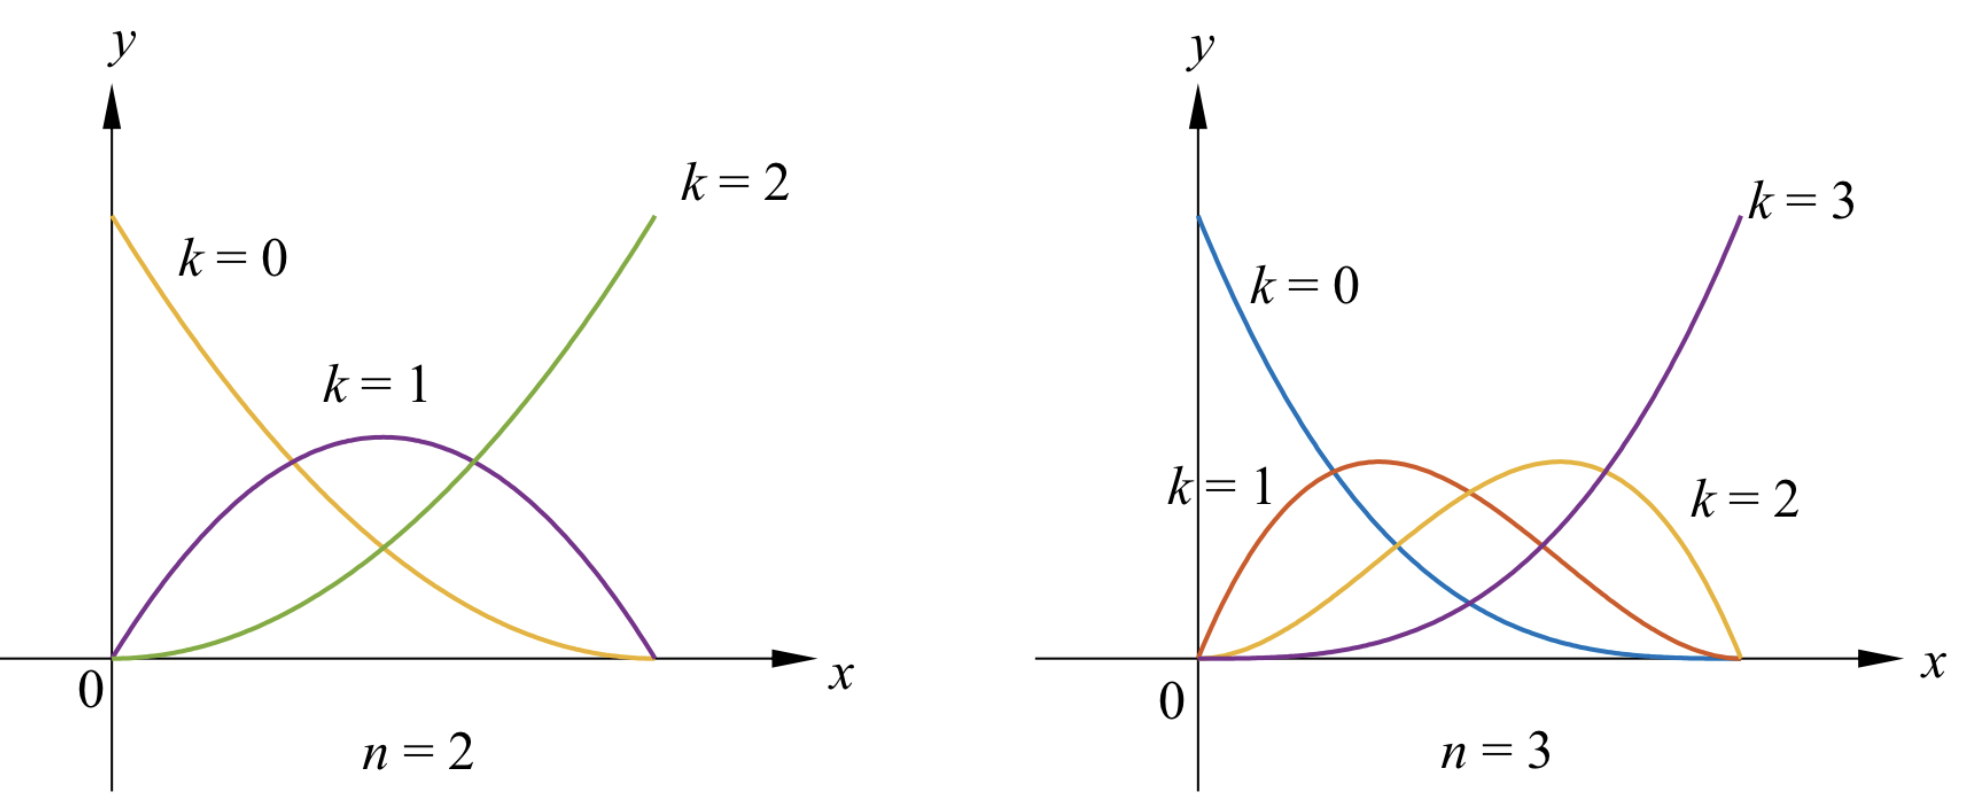
\includegraphics[scale=0.2]{Picture65.png}
\caption{The polynomials $\di p_{n,k}(x)=\binom{n}{k}x^k(1-x)^{n-k}$ when $n=2$ and $n=3$, for all $0\leq k\leq n$.\fa}\label{figure65}
 
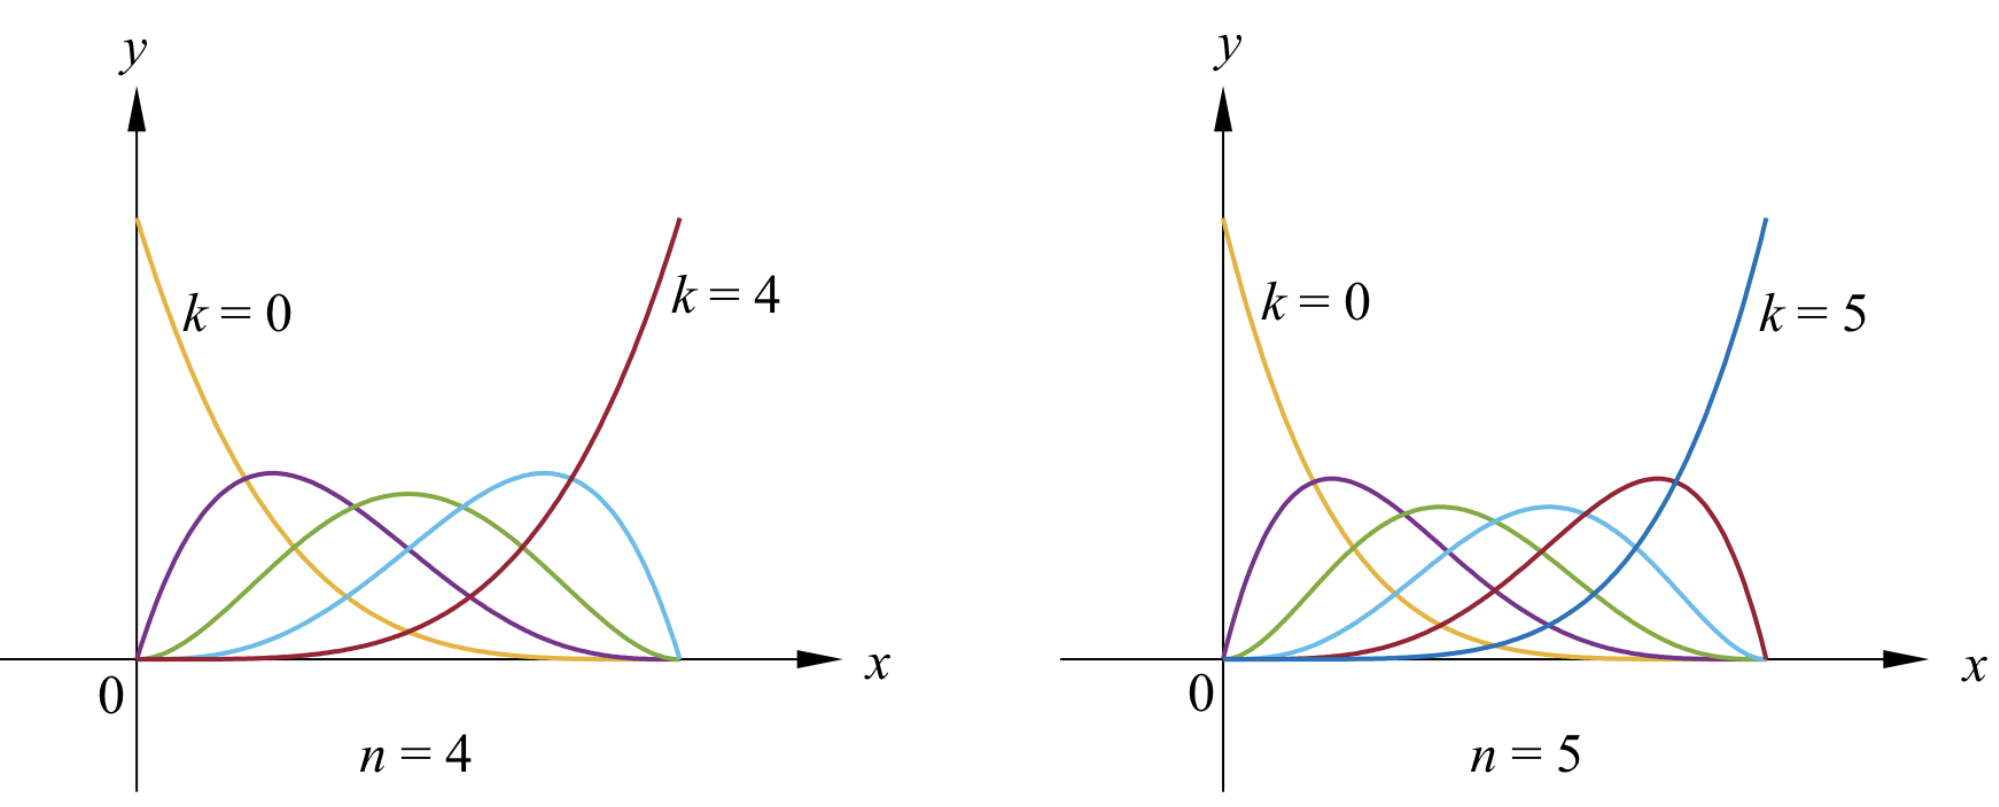
\includegraphics[scale=0.2]{Picture66.png}
\caption{The polynomials $\di  p_{n,k}(x)=\binom{n}{k}x^k(1-x)^{n-k}$ when $n=4$ and $n=5$, for all $0\leq k\leq n$.\fa}\label{figure66}
\end{figure}

\begin{figure}[ht]
\centering
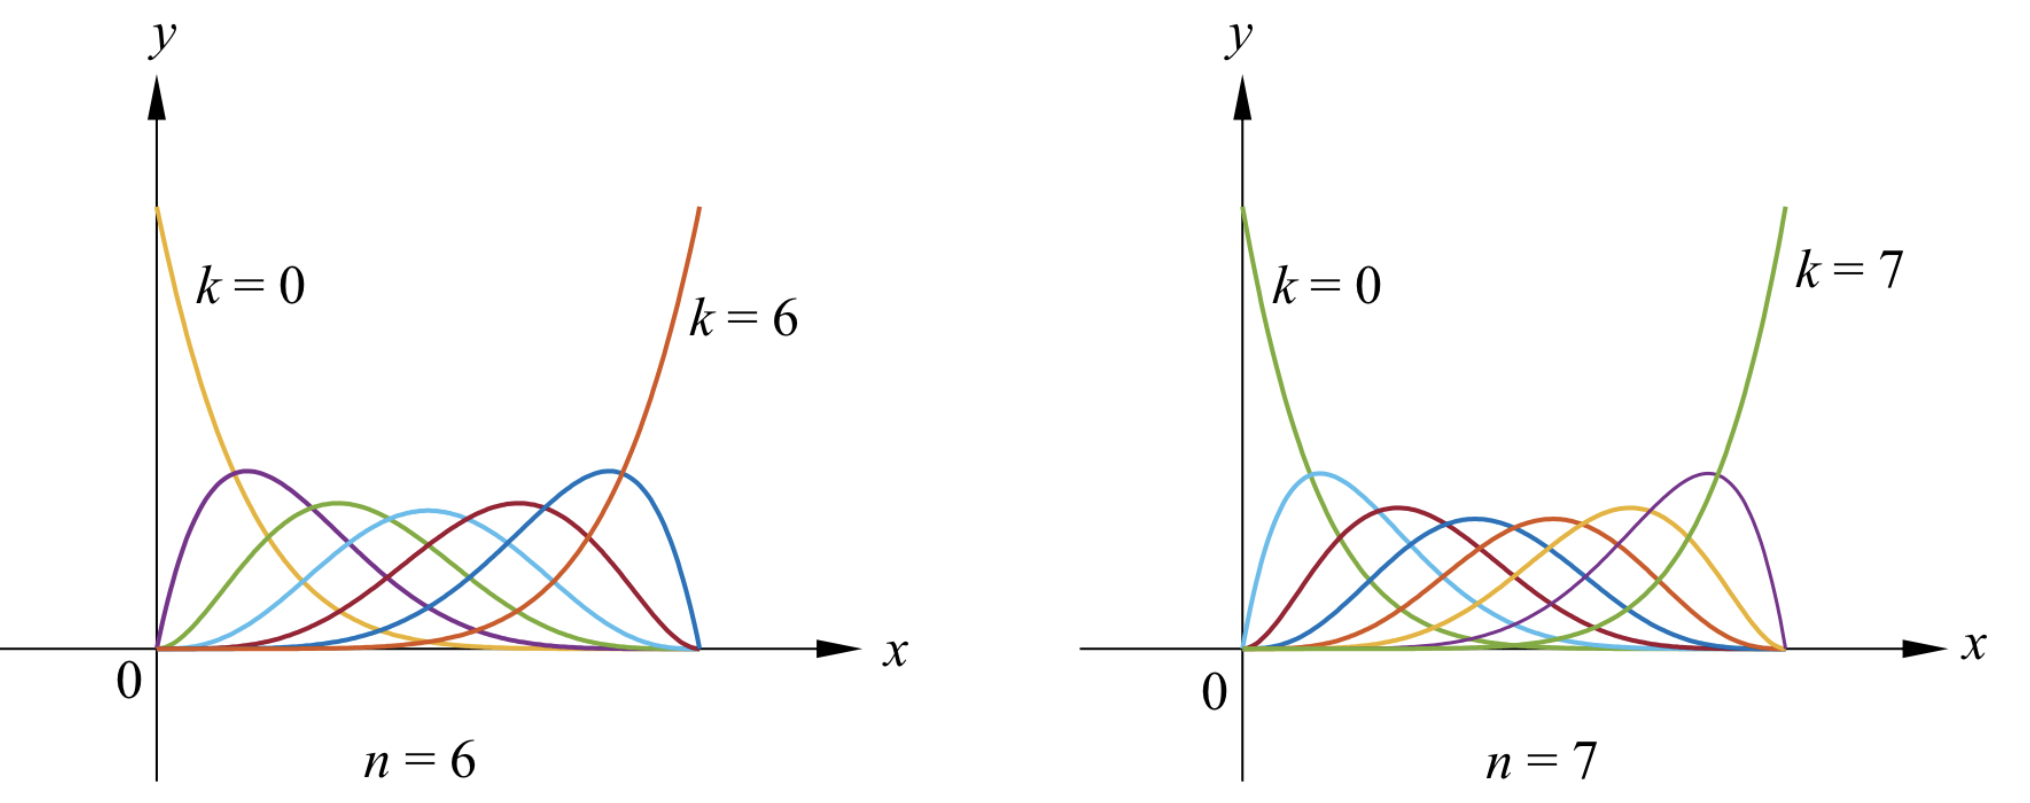
\includegraphics[scale=0.2]{Picture67.png}
\caption{The polynomials $\di  p_{n,k}(x)=\binom{n}{k}x^k(1-x)^{n-k}$ when $n=6$ and $n=7$, for all $0\leq k\leq n$.\fa}\label{figure67}
\end{figure}

Now we come to our main theorem.
\begin{theorem}{Weierstrass Approximation Theorem}
Let $f:[a,b]\to\mathbb{R}$ be a continuous function defined on $[a, b]$. Given $\varepsilon>0$, there is a polynomial $p(x)$ such that
\[|f(x)-p(x)|<\varepsilon\hspace{1cm}\text{for all}\;x\in [a,b].\]
\end{theorem}
\begin{myproof}{Proof}
We first consider the case where $[a,b]=[0,1]$. Since $f:[0,1]\to\mathbb{R}$ is continuous on a closed and bounded interval, it is uniformly continuous and bounded. The boundeness of $f$ implies that there is a positive number $M$ such that
\[|f(x)|\leq M\hspace{1cm}\text{for all}\;x\in [0,1].\] Given $\varepsilon>0$, since $f$ is uniformly continuous, there is a $\delta>0$ such that for all $x_1$ and $x_2$ in $[0,1]$, if $|x_1-x_2|<\delta$, then 
\[|f(x_1)-f(x_2)|<\frac{\varepsilon}{2}.\]  

For any positive integer  $n$, we construct a polynomial $p_n(x)$ to be a polynomial of degree at most $n$ given by the following linear combination of Bernstein basis polynomials.\bp

\[p_n(x)=\sum_{k=0}^n f\left(\frac{k}{n}\right)p_{n,k}(x)=\sum_{k=0}^n f\left(\frac{k}{n}\right)\binom{n}{k}x^k(1-x)^{n-k}.\]  Let us estimate the supremum of $|f(x)-p_n(x)|$ on $[0,1]$. For fixed $x\in [0,1]$, part (a) in Lemma \ref{230309_14} implies that
\[
f(x)-p_n(x)=\sum_{k=0}\left(f(x)-f\left(\frac{k}{n}\right)\right)\binom{n}{k}x^k(1-x)^{n-k}.\] 
 
Since $x^k(1-x)^{n-k}\geq 0$ for all $x\in [0, 1]$ and all $n\geq k\geq 0$, triangle inequality gives
\[
\left|f(x)-p_n(x)\right|\leq \sum_{k=0}\left|f(x)-f\left(\frac{k}{n}\right)\right|\binom{n}{k}x^k(1-x)^{n-k}.\]  
For  $0\leq k\leq n$, if  $\di \left|x-\frac{k}{n}\right|<\delta$, then 
\[\left|f(x)-f\left(\frac{k}{n}\right)\right|<\frac{\varepsilon}{2}.\]
If $\di \left|x-\frac{k}{n}\right|\geq \delta$, then
\[\left|f(x)-f\left(\frac{k}{n}\right)\right|\leq \left|f(x)\right|+\left|f\left(\frac{k}{n}\right)\right|\leq 2M\leq \frac{2M}{\delta^2}\left(x-\frac{k}{n}\right)^2.\]In any case, we find that
\[\left|f(x)-f\left(\frac{k}{n}\right)\right|<\frac{\varepsilon}{2}+\frac{2M}{\delta^2}\left(x-\frac{k}{n}\right)^2\hspace{1cm}\text{for all}\;0\leq k\leq n.\]
Therefore,
\[
\left|f(x)-p_n(x)\right|  < \sum_{k=0}^n\left[\frac{\varepsilon}{2}+\frac{2M}{\delta^2}\left(x-\frac{k}{n}\right)^2\right]\binom{n}{k}x^k(1-x)^{n-k}.
\]By Lemma \ref{230309_14}, and the fact that
\[0\leq x(1-x)\leq\frac{1}{4}\hspace{1cm}\text{for all}\;0\leq x\leq 1,\]
\bp
we find that
\[\left|f(x)-p_n(x)\right|  <\frac{\varepsilon}{2}+\frac{2M}{\delta^2}\frac{x(1-x)}{n}\leq \frac{\varepsilon}{2}+\frac{M}{2\delta^2n}.\]
If 
$\di n\geq \frac{M}{\varepsilon\delta^2}$, 
then
$\di \frac{M}{2\delta^2n}\leq\frac{\varepsilon}{2}$.
For any such $n$, we find that
\[\left|f(x)-p_n(x)\right|  <\varepsilon\hspace{1cm}\text{for all}\;0\leq x\leq 1.\]
This completes the proof when $[a,b]=[0,1]$. 

  For general $[a,b]$, let $u:[0,1]\to\mathbb{R}$ be the polynomial function $u(t)=a+t(b-a)$. This is a continuous function mapping $[0,1]$ bijectively onto $[a,b]$. The inverse is the continuous function $u^{-1}(x)=\di\frac{x-a}{b-a}$. The function $g=f\circ u:[0,1]\to\mathbb{R}$, being a composition of continuous functions, is continuous.  By what we have proved above, given $\varepsilon>0$, there is a polynomial $q(t)$ so that 
\[|f(u(t))-q(t)|<\varepsilon\hspace{1cm}\text{for all}\;t\in [0,1].\]
Let 
\[p(x)=q(u^{-1}(x))=q\left(\frac{x-a}{b-a}\right).\] Then $p(x)$ is also a polynomial, and $p(u(t))=q(t)$. Therefore,
\[|f(u(t))-p(u(t))|<\varepsilon\hspace{1cm}\text{for all}\;t\in [0,1],\]which implies that
\[|f(x)-p(x)|<\varepsilon \hspace{1cm}\text{for all}\;x\in [a,b].\]This completes the proof of the Weierstrass approximation theorem for the general  case.

\end{myproof}
\begin{figure}[ht]
\centering
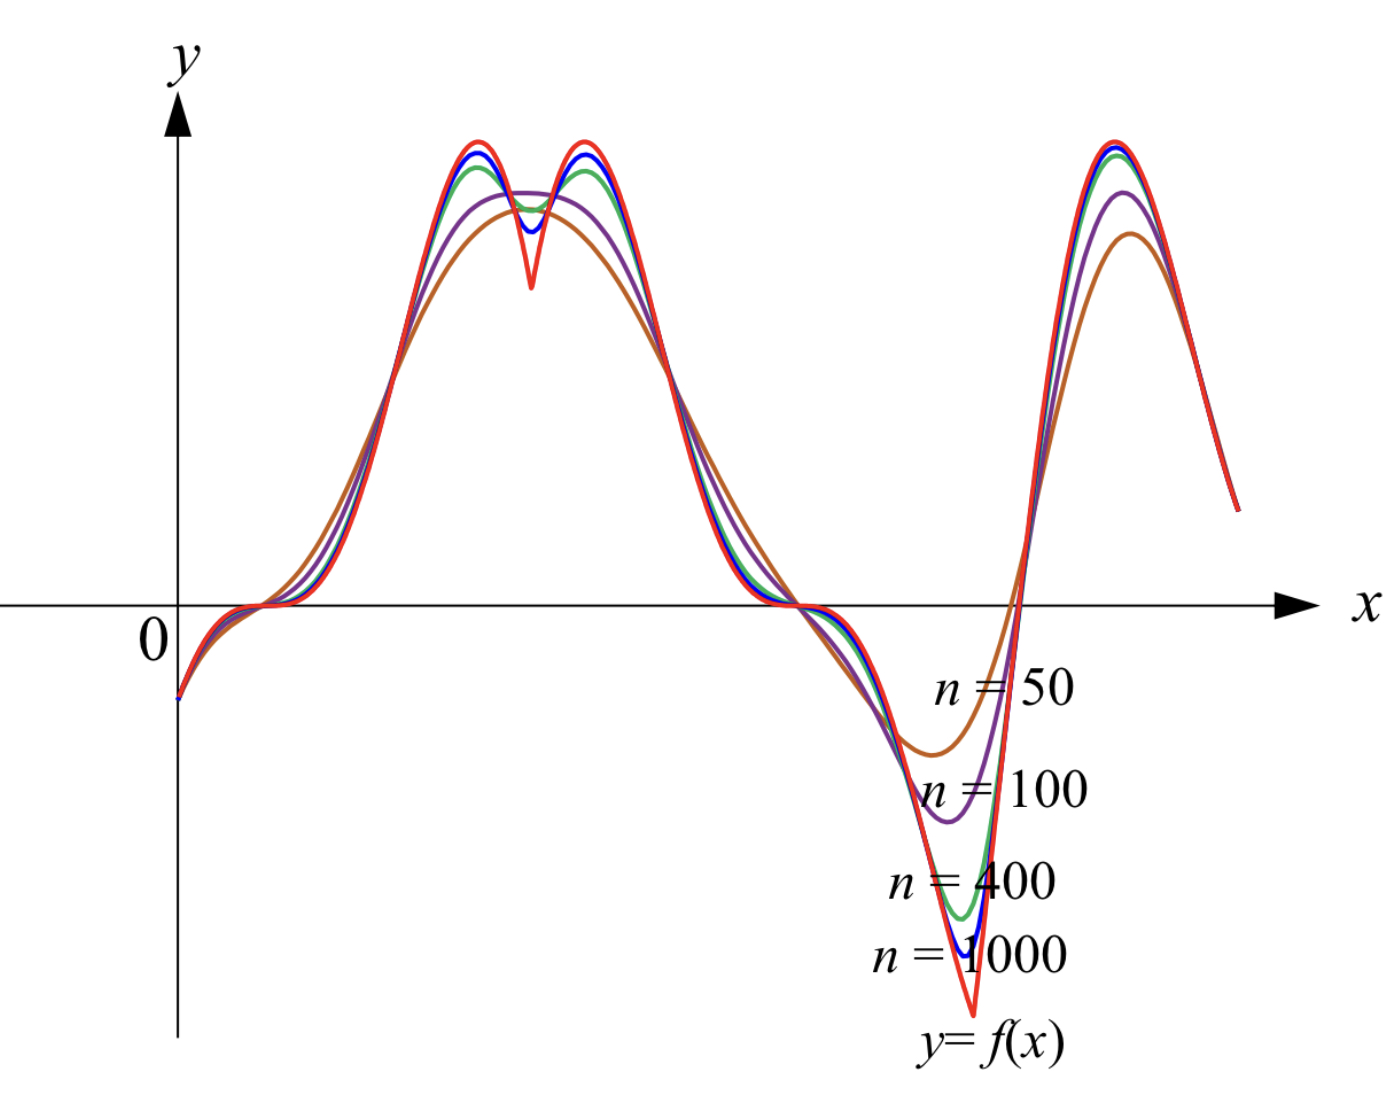
\includegraphics[scale=0.2]{Picture68.png}
\caption{Approximations of the continuous function $f(x)$ by the polynomials $p_n(x)$, where $f(x)=\di 3\sin( 4\pi|x-1/3|)+2\sin (6\pi|x-3/4|)$.\fa}\label{figure68}
\end{figure}
~
 
One cannot extend the Weierstrass approximation theorem to the case where $f:I\to\mathbb{R}$ is a continuous function defined on an unbounded interval $I$.  This is because a non-constant polynomial would approach $\infty$ or $-\infty$ when $x$ approaches $\infty$ or $-\infty$. However, there are bounded continuous functions defined on unbounded intervals. For example, the function
\[f(x)=\frac{x}{x^2+1}\] is a bounded continuous function defined on $\mathbb{R}$.

 



\begin{remark}
{}

In probability theory, a binomial random variable $X$ with parameters $n$ and $p$ counts the number of successes in $n$ independent and identical Bernoulli trials, each has a probability $p\in (0,1)$ of being a success.  $X$ can take integer values between $0$ and $n$. The probability that $X=k$ is
\[P(X=k)=\binom{n}{k}p^k(1-p)^{n-k},\quad 0\leq k\leq n.\]
The identity in (a) of Lemma \ref{230309_14} amounts to
\[\sum_{k=0}^n \binom{n}{k}p^k(1-p)^k=1,\]
\end{remark}\begin{highlight}{}
which reflects that the total probability is 1. The identity in part (b) gives 
\[E(X)=\sum_{k=0}^n k\binom{n}{k}p^k(1-p)^k=np,\]

which is the expected value of a binomial  random variable $X$ with parameters $n$ and $p$. The identity in part (c) gives
\[E(X^2)=\sum_{k=0}^n k^2\binom{n}{k}p^k(1-p)^k=n^2p^2+np(1-p).\] Together with the identity in part (b),  the variance of $X$ is given by
\begin{align*}\text{Var}\,(X)&=E(X^2)-E(X)^2 =n^2p^2+np(1-p)-n^2p^2=np(1-p).\end{align*}In fact, the variance of a random variable $X$ is defined as
\[\text{Var}\,(X)=E([X-E(X)]^2).\]The identity in part (d) of Lemma \ref{230309_14} is just another way of computing the variance.  Using part (d), we have
\begin{align*}\text{Var}\,(X)&= \sum_{k=0}^n (k-np)^2\binom{n}{k}p^k(1-p)^k\\&=n^2 \sum_{k=0}^n \left(\frac{k}{n}-p\right)^2\binom{n}{k}p^k(1-p)^k=np(1-p).\end{align*}

\end{highlight}




